% Generated by Sphinx.
\def\sphinxdocclass{report}
\documentclass[letterpaper,10pt,english]{sphinxmanual}
\usepackage[utf8]{inputenc}
\DeclareUnicodeCharacter{00A0}{\nobreakspace}
\usepackage{cmap}
\usepackage[T1]{fontenc}
\usepackage{babel}
\usepackage{times}
\usepackage[Sonny]{fncychap}
\usepackage{longtable}
\usepackage{sphinx}
\usepackage{multirow}


\addto\captionsenglish{\renewcommand{\figurename}{Fig. }}
\addto\captionsenglish{\renewcommand{\tablename}{Table }}
\floatname{literal-block}{Listing }

\setcounter{tocdepth}{2}

\title{MapMint, Guide utilisateur}
\date{August 01, 2018}
\release{1.2}
\author{Balley Beye, Nicolas Bozon, Dame Dieng, Gérald Fenoy, \\Abdoulaye Samb}
\newcommand{\sphinxlogo}{
\includegraphics{mm-logo.png}\par}
\renewcommand{\releasename}{Release}
\makeindex

\makeatletter
\def\PYG@reset{\let\PYG@it=\relax \let\PYG@bf=\relax%
    \let\PYG@ul=\relax \let\PYG@tc=\relax%
    \let\PYG@bc=\relax \let\PYG@ff=\relax}
\def\PYG@tok#1{\csname PYG@tok@#1\endcsname}
\def\PYG@toks#1+{\ifx\relax#1\empty\else%
    \PYG@tok{#1}\expandafter\PYG@toks\fi}
\def\PYG@do#1{\PYG@bc{\PYG@tc{\PYG@ul{%
    \PYG@it{\PYG@bf{\PYG@ff{#1}}}}}}}
\def\PYG#1#2{\PYG@reset\PYG@toks#1+\relax+\PYG@do{#2}}

\expandafter\def\csname PYG@tok@gd\endcsname{\def\PYG@tc##1{\textcolor[rgb]{0.63,0.00,0.00}{##1}}}
\expandafter\def\csname PYG@tok@gu\endcsname{\let\PYG@bf=\textbf\def\PYG@tc##1{\textcolor[rgb]{0.50,0.00,0.50}{##1}}}
\expandafter\def\csname PYG@tok@gt\endcsname{\def\PYG@tc##1{\textcolor[rgb]{0.00,0.27,0.87}{##1}}}
\expandafter\def\csname PYG@tok@gs\endcsname{\let\PYG@bf=\textbf}
\expandafter\def\csname PYG@tok@gr\endcsname{\def\PYG@tc##1{\textcolor[rgb]{1.00,0.00,0.00}{##1}}}
\expandafter\def\csname PYG@tok@cm\endcsname{\let\PYG@it=\textit\def\PYG@tc##1{\textcolor[rgb]{0.25,0.50,0.56}{##1}}}
\expandafter\def\csname PYG@tok@vg\endcsname{\def\PYG@tc##1{\textcolor[rgb]{0.73,0.38,0.84}{##1}}}
\expandafter\def\csname PYG@tok@vi\endcsname{\def\PYG@tc##1{\textcolor[rgb]{0.73,0.38,0.84}{##1}}}
\expandafter\def\csname PYG@tok@mh\endcsname{\def\PYG@tc##1{\textcolor[rgb]{0.13,0.50,0.31}{##1}}}
\expandafter\def\csname PYG@tok@cs\endcsname{\def\PYG@tc##1{\textcolor[rgb]{0.25,0.50,0.56}{##1}}\def\PYG@bc##1{\setlength{\fboxsep}{0pt}\colorbox[rgb]{1.00,0.94,0.94}{\strut ##1}}}
\expandafter\def\csname PYG@tok@ge\endcsname{\let\PYG@it=\textit}
\expandafter\def\csname PYG@tok@vc\endcsname{\def\PYG@tc##1{\textcolor[rgb]{0.73,0.38,0.84}{##1}}}
\expandafter\def\csname PYG@tok@il\endcsname{\def\PYG@tc##1{\textcolor[rgb]{0.13,0.50,0.31}{##1}}}
\expandafter\def\csname PYG@tok@go\endcsname{\def\PYG@tc##1{\textcolor[rgb]{0.20,0.20,0.20}{##1}}}
\expandafter\def\csname PYG@tok@cp\endcsname{\def\PYG@tc##1{\textcolor[rgb]{0.00,0.44,0.13}{##1}}}
\expandafter\def\csname PYG@tok@gi\endcsname{\def\PYG@tc##1{\textcolor[rgb]{0.00,0.63,0.00}{##1}}}
\expandafter\def\csname PYG@tok@gh\endcsname{\let\PYG@bf=\textbf\def\PYG@tc##1{\textcolor[rgb]{0.00,0.00,0.50}{##1}}}
\expandafter\def\csname PYG@tok@ni\endcsname{\let\PYG@bf=\textbf\def\PYG@tc##1{\textcolor[rgb]{0.84,0.33,0.22}{##1}}}
\expandafter\def\csname PYG@tok@nl\endcsname{\let\PYG@bf=\textbf\def\PYG@tc##1{\textcolor[rgb]{0.00,0.13,0.44}{##1}}}
\expandafter\def\csname PYG@tok@nn\endcsname{\let\PYG@bf=\textbf\def\PYG@tc##1{\textcolor[rgb]{0.05,0.52,0.71}{##1}}}
\expandafter\def\csname PYG@tok@no\endcsname{\def\PYG@tc##1{\textcolor[rgb]{0.38,0.68,0.84}{##1}}}
\expandafter\def\csname PYG@tok@na\endcsname{\def\PYG@tc##1{\textcolor[rgb]{0.25,0.44,0.63}{##1}}}
\expandafter\def\csname PYG@tok@nb\endcsname{\def\PYG@tc##1{\textcolor[rgb]{0.00,0.44,0.13}{##1}}}
\expandafter\def\csname PYG@tok@nc\endcsname{\let\PYG@bf=\textbf\def\PYG@tc##1{\textcolor[rgb]{0.05,0.52,0.71}{##1}}}
\expandafter\def\csname PYG@tok@nd\endcsname{\let\PYG@bf=\textbf\def\PYG@tc##1{\textcolor[rgb]{0.33,0.33,0.33}{##1}}}
\expandafter\def\csname PYG@tok@ne\endcsname{\def\PYG@tc##1{\textcolor[rgb]{0.00,0.44,0.13}{##1}}}
\expandafter\def\csname PYG@tok@nf\endcsname{\def\PYG@tc##1{\textcolor[rgb]{0.02,0.16,0.49}{##1}}}
\expandafter\def\csname PYG@tok@si\endcsname{\let\PYG@it=\textit\def\PYG@tc##1{\textcolor[rgb]{0.44,0.63,0.82}{##1}}}
\expandafter\def\csname PYG@tok@s2\endcsname{\def\PYG@tc##1{\textcolor[rgb]{0.25,0.44,0.63}{##1}}}
\expandafter\def\csname PYG@tok@nt\endcsname{\let\PYG@bf=\textbf\def\PYG@tc##1{\textcolor[rgb]{0.02,0.16,0.45}{##1}}}
\expandafter\def\csname PYG@tok@nv\endcsname{\def\PYG@tc##1{\textcolor[rgb]{0.73,0.38,0.84}{##1}}}
\expandafter\def\csname PYG@tok@s1\endcsname{\def\PYG@tc##1{\textcolor[rgb]{0.25,0.44,0.63}{##1}}}
\expandafter\def\csname PYG@tok@ch\endcsname{\let\PYG@it=\textit\def\PYG@tc##1{\textcolor[rgb]{0.25,0.50,0.56}{##1}}}
\expandafter\def\csname PYG@tok@m\endcsname{\def\PYG@tc##1{\textcolor[rgb]{0.13,0.50,0.31}{##1}}}
\expandafter\def\csname PYG@tok@gp\endcsname{\let\PYG@bf=\textbf\def\PYG@tc##1{\textcolor[rgb]{0.78,0.36,0.04}{##1}}}
\expandafter\def\csname PYG@tok@sh\endcsname{\def\PYG@tc##1{\textcolor[rgb]{0.25,0.44,0.63}{##1}}}
\expandafter\def\csname PYG@tok@ow\endcsname{\let\PYG@bf=\textbf\def\PYG@tc##1{\textcolor[rgb]{0.00,0.44,0.13}{##1}}}
\expandafter\def\csname PYG@tok@sx\endcsname{\def\PYG@tc##1{\textcolor[rgb]{0.78,0.36,0.04}{##1}}}
\expandafter\def\csname PYG@tok@bp\endcsname{\def\PYG@tc##1{\textcolor[rgb]{0.00,0.44,0.13}{##1}}}
\expandafter\def\csname PYG@tok@c1\endcsname{\let\PYG@it=\textit\def\PYG@tc##1{\textcolor[rgb]{0.25,0.50,0.56}{##1}}}
\expandafter\def\csname PYG@tok@o\endcsname{\def\PYG@tc##1{\textcolor[rgb]{0.40,0.40,0.40}{##1}}}
\expandafter\def\csname PYG@tok@kc\endcsname{\let\PYG@bf=\textbf\def\PYG@tc##1{\textcolor[rgb]{0.00,0.44,0.13}{##1}}}
\expandafter\def\csname PYG@tok@c\endcsname{\let\PYG@it=\textit\def\PYG@tc##1{\textcolor[rgb]{0.25,0.50,0.56}{##1}}}
\expandafter\def\csname PYG@tok@mf\endcsname{\def\PYG@tc##1{\textcolor[rgb]{0.13,0.50,0.31}{##1}}}
\expandafter\def\csname PYG@tok@err\endcsname{\def\PYG@bc##1{\setlength{\fboxsep}{0pt}\fcolorbox[rgb]{1.00,0.00,0.00}{1,1,1}{\strut ##1}}}
\expandafter\def\csname PYG@tok@mb\endcsname{\def\PYG@tc##1{\textcolor[rgb]{0.13,0.50,0.31}{##1}}}
\expandafter\def\csname PYG@tok@ss\endcsname{\def\PYG@tc##1{\textcolor[rgb]{0.32,0.47,0.09}{##1}}}
\expandafter\def\csname PYG@tok@sr\endcsname{\def\PYG@tc##1{\textcolor[rgb]{0.14,0.33,0.53}{##1}}}
\expandafter\def\csname PYG@tok@mo\endcsname{\def\PYG@tc##1{\textcolor[rgb]{0.13,0.50,0.31}{##1}}}
\expandafter\def\csname PYG@tok@kd\endcsname{\let\PYG@bf=\textbf\def\PYG@tc##1{\textcolor[rgb]{0.00,0.44,0.13}{##1}}}
\expandafter\def\csname PYG@tok@mi\endcsname{\def\PYG@tc##1{\textcolor[rgb]{0.13,0.50,0.31}{##1}}}
\expandafter\def\csname PYG@tok@kn\endcsname{\let\PYG@bf=\textbf\def\PYG@tc##1{\textcolor[rgb]{0.00,0.44,0.13}{##1}}}
\expandafter\def\csname PYG@tok@cpf\endcsname{\let\PYG@it=\textit\def\PYG@tc##1{\textcolor[rgb]{0.25,0.50,0.56}{##1}}}
\expandafter\def\csname PYG@tok@kr\endcsname{\let\PYG@bf=\textbf\def\PYG@tc##1{\textcolor[rgb]{0.00,0.44,0.13}{##1}}}
\expandafter\def\csname PYG@tok@s\endcsname{\def\PYG@tc##1{\textcolor[rgb]{0.25,0.44,0.63}{##1}}}
\expandafter\def\csname PYG@tok@kp\endcsname{\def\PYG@tc##1{\textcolor[rgb]{0.00,0.44,0.13}{##1}}}
\expandafter\def\csname PYG@tok@w\endcsname{\def\PYG@tc##1{\textcolor[rgb]{0.73,0.73,0.73}{##1}}}
\expandafter\def\csname PYG@tok@kt\endcsname{\def\PYG@tc##1{\textcolor[rgb]{0.56,0.13,0.00}{##1}}}
\expandafter\def\csname PYG@tok@sc\endcsname{\def\PYG@tc##1{\textcolor[rgb]{0.25,0.44,0.63}{##1}}}
\expandafter\def\csname PYG@tok@sb\endcsname{\def\PYG@tc##1{\textcolor[rgb]{0.25,0.44,0.63}{##1}}}
\expandafter\def\csname PYG@tok@k\endcsname{\let\PYG@bf=\textbf\def\PYG@tc##1{\textcolor[rgb]{0.00,0.44,0.13}{##1}}}
\expandafter\def\csname PYG@tok@se\endcsname{\let\PYG@bf=\textbf\def\PYG@tc##1{\textcolor[rgb]{0.25,0.44,0.63}{##1}}}
\expandafter\def\csname PYG@tok@sd\endcsname{\let\PYG@it=\textit\def\PYG@tc##1{\textcolor[rgb]{0.25,0.44,0.63}{##1}}}

\def\PYGZbs{\char`\\}
\def\PYGZus{\char`\_}
\def\PYGZob{\char`\{}
\def\PYGZcb{\char`\}}
\def\PYGZca{\char`\^}
\def\PYGZam{\char`\&}
\def\PYGZlt{\char`\<}
\def\PYGZgt{\char`\>}
\def\PYGZsh{\char`\#}
\def\PYGZpc{\char`\%}
\def\PYGZdl{\char`\$}
\def\PYGZhy{\char`\-}
\def\PYGZsq{\char`\'}
\def\PYGZdq{\char`\"}
\def\PYGZti{\char`\~}
% for compatibility with earlier versions
\def\PYGZat{@}
\def\PYGZlb{[}
\def\PYGZrb{]}
\makeatother

\renewcommand\PYGZsq{\textquotesingle}

\begin{document}

\maketitle
\tableofcontents
\phantomsection\label{index::doc}


Welcome to the user guide of the \href{http://mapmint.com}{MapMint} application.

\begin{notice}{note}{Note:}
Le guide utilisateur est aussi disponible aux formats
PDF 
\includegraphics{pdf.png}  et ePub 
\includegraphics{epub.png}
\end{notice}


\chapter{Introduction}
\label{introduction/index:table-des-matieres}\label{introduction/index:home}\label{introduction/index::doc}\label{introduction/index:dashboard}\label{introduction/index:introduction}

\section{Overview}
\label{introduction/introduction:generalites}\label{introduction/introduction::doc}\label{introduction/introduction:userguidegeneral}

\subsection{What is MapMint?}
\label{introduction/introduction:quest-ce-que-mapmint}
MapMint is a geographic information system (GIS) software on the Internet designed to facilitate the deployment of  \textbf{spatial data infrastructures} (SDI).

MapMint is for individuals and organizations wishing to manage and optimize SDI establishment and deployment of dynamic mapping applications. The application centralizes and simplifies a number of GIS and WebGIS functionality. The different levels of user rights divide tasks according to public (system administrators, GIS specialists, GIS technicians, cartographers, webmasters ...).


\subsection{What allows MapMint?}
\label{introduction/introduction:que-permet-mapmint}
MapMint allows multiple tasks relating to the implementation of an SDI from a modular and user-friendly administration interface. The user can MapMint, according to his rights:
\begin{itemize}
\item {} 
Import and store vector and raster GIS data

\item {} 
Query database server and WMS / WFS external

\item {} 
Publish geographic data in the form of WMS, WFS and WMTS

\item {} 
Treat, edit and Data Sources style

\item {} 
Compose and save maps in the form of projects (mapfiles)

\item {} 
Configure and generate mapping applications

\item {} 
Configure and run a cartographic portal

\item {} 
View and share maps

\end{itemize}


\subsection{How MapMint works?}
\label{introduction/introduction:comment-fonctionne-mapmint}
MapMint includes several \href{http://mapmint.com/en/Components}{free software} in a complete and coherent web mapping platform, whose operation is based on the use of \href{http://mapmint.com/en/Components}{open standards} geomatics and internet.

At the heart of MapMint we have the \href{http://zoo-project.org}{ZOO-Project}, an application to simply and efficiently deploy WPS (\href{http://www.opengeospatial.org/standards/wps}{Web Processing Service}) data processing. A set of web services is available MapMint, from simple display of a web page in the application to complex geographical treatments.

On the other types of web services are implemented, including visualization and querying spatial data, WMS (\href{http://www.opengeospatial.org/standards/wms}{Web Map Service}). Access to geographic data in vector format is via the WFS (\href{http://www.opengeospatial.org/standards/wfs}{Web Feature Service}) or access to image data via WCS (\href{http://www.opengeospatial.org/standards/wcs}{Web Coverage Service}). All these web services are provided by \href{http://mapserver.org}{MapServer}. The various files necessary for the functioning of MapServer and dynamic mapping applications are managed by MapMint services which provided a friendly interface for interact with these web services.

ZOO-Project and MapServer applications based on an Apache web server to access the application via HTTP and HTTPS communication protocols.

\begin{notice}{note}{Note:}
In a Windows environment, IIS can be used instead of Apache
\end{notice}

All the documents produced by the application, such as when using the pdf document production client module, use templates to odt file (\href{https://www.oasis-open.org/committees/tc\_home.php?wg\_abbrev=office}{OpenDocumentText}). Document production is based on UNO (\href{https://www.openoffice.org/udk/common/man/uno.html}{Universal Network Object}) to interact with a \href{http://www.libreoffice.org/}{LibreOffice} server.

An FTP server (eg ProFTPd) is generally associated with an instance of MapMint making available the directory \code{dataPath/ftp} order to file on the server large files or manage the templates in it.

Some services dedicated to data classification using the \href{http://r-project.org}{R} library, all geographic data is read via the use of  \href{http://www.gdal.org}{GDAL}, the QRCodes are generated using the \href{https://fukuchi.org/works/qrencode/}{QREncode} library. Some specific Python modules are also needed, and cssmin JSMin to minimize the size of JavaScript and CSS files generated by the application.

An overview of the architecture of MapMint is presented below.

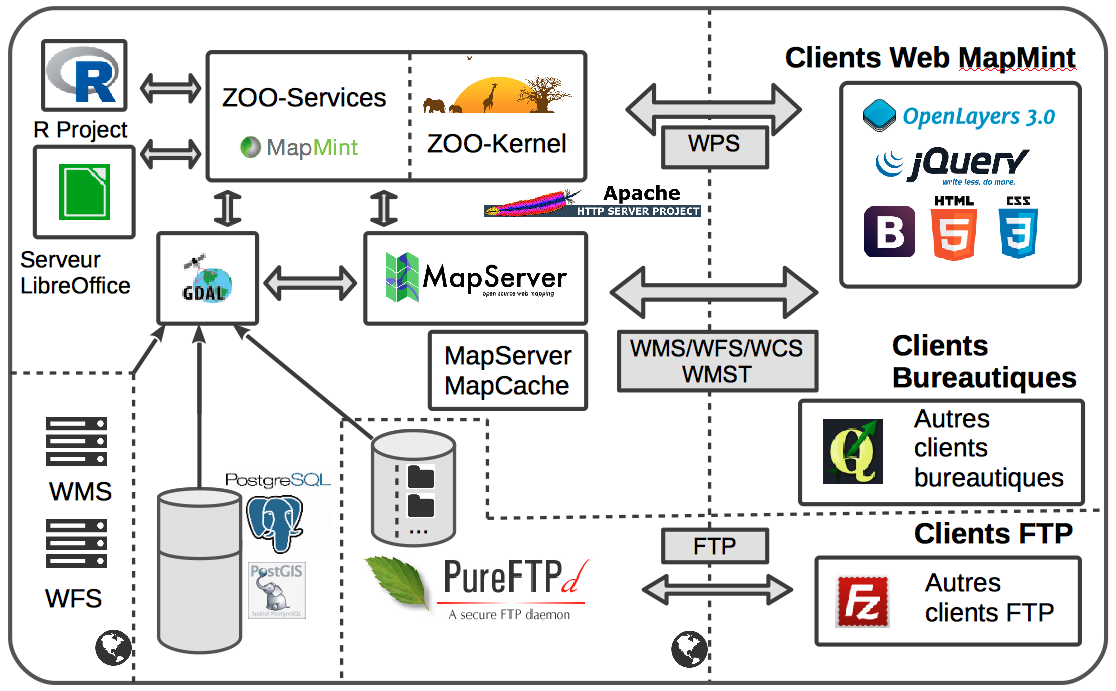
\includegraphics{mapmint-arch.png}

The interoperability of MapMint is provided by the standards used and implemented . It is thus possible to interact with data and services MapMint not only from the application accessible from a web browser but also from a desktop client type QGIS for example.

\begin{notice}{note}{Note:}
To use WPS, WPS, download the plugin available \href{http://geolabs.fr/plugins.xml}{here}.
\end{notice}

You can find more general information on the website of \href{http://mapmint.com/en/}{MapMint}


\section{Install MapMint}
\label{introduction/installmapmint:installer-mapmint}\label{introduction/installmapmint::doc}\label{introduction/installmapmint:introduction-installmapmint}\setbox0\vbox{
\begin{minipage}{0.95\linewidth}
\textbf{Table of Contents}

\medskip

\begin{itemize}
\item {} 
\phantomsection\label{introduction/installmapmint:id1}{\hyperref[introduction/installmapmint:installer-mapmint]{\emph{Install MapMint}}}
\begin{itemize}
\item {} 
\phantomsection\label{introduction/installmapmint:id2}{\hyperref[introduction/installmapmint:prerequis]{\emph{Prerequisites}}}
\begin{itemize}
\item {} 
\phantomsection\label{introduction/installmapmint:id3}{\hyperref[introduction/installmapmint:paquets-et-modules-python]{\emph{Python packages and modules}}}

\item {} 
\phantomsection\label{introduction/installmapmint:id4}{\hyperref[introduction/installmapmint:telecharger-ansible-et-les-scripts-d-installation]{\emph{Ansible download and install scripts}}}

\item {} 
\phantomsection\label{introduction/installmapmint:id5}{\hyperref[introduction/installmapmint:creation-d-une-cle-ssh]{\emph{Generating an SSH key}}}

\end{itemize}

\item {} 
\phantomsection\label{introduction/installmapmint:id6}{\hyperref[introduction/installmapmint:installation]{\emph{Installation}}}

\end{itemize}

\end{itemize}
\end{minipage}}
\begin{center}\setlength{\fboxsep}{5pt}\shadowbox{\box0}\end{center}

MapMint The application can be installed very simply using \href{http://ansible.com}{Ansible scripts}. It is thus possible to deploy several instances of MapMint through the use of the \code{ansible-playbook}. In this part of the installation will affect only a single instance, the local host that uses a GNU/Linux distribution: Ubuntu 14.03.3 LTS.


\subsection{Prerequisites}
\label{introduction/installmapmint:prerequis}

\subsubsection{Python packages and modules}
\label{introduction/installmapmint:paquets-et-modules-python}
Before you can install MapMint using Ansible scripts, it is necessary to ensure the presence of some Ubuntu packages and specific Python modules.

\begin{Verbatim}[commandchars=\\\{\}]
sudo apt\PYGZhy{}get install git python\PYGZhy{}setuptools openssh\PYGZhy{}server
sudo easy\PYGZus{}install pip
sudo pip install paramiko PyYAML Jinja2 httplib2 six
\end{Verbatim}


\subsubsection{Ansible download and install scripts}
\label{introduction/installmapmint:telecharger-ansible-et-les-scripts-d-installation}
It is necessary to download and Ansible specific scripts installation MapMint. To do this, use the following commands.

\begin{Verbatim}[commandchars=\\\{\}]
cd
mkdir mm\PYGZhy{}install
cd mm\PYGZhy{}install
git clone git://github.com/ansible/ansible.git \PYGZhy{}\PYGZhy{}recursive
git clone git://github.com/mapmint/ansible\PYGZhy{}roles mapmint\PYGZhy{}setup
\end{Verbatim}


\subsubsection{Generating an SSH key}
\label{introduction/installmapmint:creation-d-une-cle-ssh}
So your user can connect to the server via SSH MapMint on which to install, you must create a key to abort an automatic authentication. To do this use the following command.

\begin{Verbatim}[commandchars=\\\{\}]
mkdir \PYGZti{}/.ssh
ssh\PYGZhy{}keygen \PYGZhy{}t rsa
sudo mkdir /root/.ssh
sudo cp \PYGZti{}/.ssh/id\PYGZus{}rsa.pub /root/.ssh/authorized\PYGZus{}keys
\end{Verbatim}

\begin{notice}{warning}{Warning:}
The last command remove all authorized key server.
\end{notice}

\begin{notice}{note}{Note:}
Use a different order if you want to update the list of authorized keys.
\end{notice}


\subsection{Installation}
\label{introduction/installmapmint:installation}
Installing MapMint is fully automated via the Ansible previously downloaded scripts, so it only remains to launch. Before that, it will be necessary to set Ansible and specific scripts installation MapMint to define the name of the machine that will be used to access the instance.

Initially you will enable Ansible and define which machines you want to install MapMint. In the example presented here, the facilities will be made ​​on the local machine, so \code{localhost} .

\begin{Verbatim}[commandchars=\\\{\}]
source \PYGZti{}/mm\PYGZhy{}install/ansible/hacking/env\PYGZhy{}setup
echo \PYGZdq{}localhost\PYGZdq{} \PYGZgt{} \PYGZti{}/ansible\PYGZus{}hosts
sed \PYGZdq{}s:myhost.net:localhost:g\PYGZdq{} \PYGZhy{}i \PYGZbs{}
   \PYGZti{}/mm\PYGZhy{}install/mapmint\PYGZhy{}setup/debian/dependencies/vars/main.yml
export ANSIBLE\PYGZus{}INVENTORY=\PYGZti{}/ansible\PYGZus{}hosts
\end{Verbatim}

\begin{notice}{note}{Note:}
\code{localhost} should be replaced with the machine name or IP address allowing public access to the proceedings.
\end{notice}

It remains only to invoke the installation of MapMint with the command below.

\begin{Verbatim}[commandchars=\\\{\}]
cd \PYGZti{}/mm\PYGZhy{}install/mapmint\PYGZhy{}setup/ubuntu
ansible\PYGZhy{}playbook \PYGZhy{}s server.yml \PYGZhy{}u root
\end{Verbatim}

To access your MapMint instance, you can use the following links:
\begin{itemize}
\item {} 
{\hyperref[introduction/usemapmint:introduction-usemapmint-administration-access]{\emph{Access to administrative modules}}} : \href{http://localhost/ui/Dashboard\_bs}{http://localhost/ui/Dashboard\_bs}

\item {} 
{\hyperref[introduction/usemapmint:introduction-usemapmint-public-access]{\emph{Access to the public interface}}} : \href{http://localhost/ui/public/}{http://localhost/ui/public/}

\end{itemize}


\section{Use MapMint}
\label{introduction/usemapmint:utiliser-mapmint}\label{introduction/usemapmint:introduction-usemapmint}\label{introduction/usemapmint::doc}\setbox0\vbox{
\begin{minipage}{0.95\linewidth}
\textbf{Table of Contents}

\medskip

\begin{itemize}
\item {} 
\phantomsection\label{introduction/usemapmint:id1}{\hyperref[introduction/usemapmint:utiliser-mapmint]{\emph{Use MapMint}}}
\begin{itemize}
\item {} 
\phantomsection\label{introduction/usemapmint:id2}{\hyperref[introduction/usemapmint:acces-aux-modules-d-administration]{\emph{Access to administrative modules}}}

\item {} 
\phantomsection\label{introduction/usemapmint:id3}{\hyperref[introduction/usemapmint:formulaire-d-identification]{\emph{Identification Form}}}

\item {} 
\phantomsection\label{introduction/usemapmint:id4}{\hyperref[introduction/usemapmint:acces-a-l-interface-publique]{\emph{Access to the public interface}}}

\item {} 
\phantomsection\label{introduction/usemapmint:id5}{\hyperref[introduction/usemapmint:premiers-parametrages]{\emph{First settings}}}
\begin{itemize}
\item {} 
\phantomsection\label{introduction/usemapmint:id6}{\hyperref[introduction/usemapmint:titre-de-l-interface-publique]{\emph{Title of the public interface}}}

\item {} 
\phantomsection\label{introduction/usemapmint:id7}{\hyperref[introduction/usemapmint:carte-de-l-interface-publique]{\emph{Map of the public interface}}}

\end{itemize}

\item {} 
\phantomsection\label{introduction/usemapmint:id8}{\hyperref[introduction/usemapmint:ajouter-des-donnees]{\emph{Add data}}}

\item {} 
\phantomsection\label{introduction/usemapmint:id9}{\hyperref[introduction/usemapmint:acces-aux-donnees-et-traitements-depuis-des-clients-bureautiques]{\emph{Access to data and processes from the desktop clients}}}
\begin{itemize}
\item {} 
\phantomsection\label{introduction/usemapmint:id10}{\hyperref[introduction/usemapmint:acceder-aux-services-de-diffusion-de-donnees]{\emph{Accessing data broadcasting services}}}

\item {} 
\phantomsection\label{introduction/usemapmint:id11}{\hyperref[introduction/usemapmint:acceder-aux-services-de-traitements-de-donnees]{\emph{Access to data processing services}}}

\end{itemize}

\end{itemize}

\end{itemize}
\end{minipage}}
\begin{center}\setlength{\fboxsep}{5pt}\shadowbox{\box0}\end{center}

MapMint The application consists of an \textbf{administration interface} with various modules and a \textbf{public interface}.


\subsection{Access to administrative modules}
\label{introduction/usemapmint:acces-aux-modules-d-administration}\label{introduction/usemapmint:introduction-usemapmint-administration-access}
Depending on the settings of the {\hyperref[dashboard/configuration::doc]{\emph{\emph{Control Panel}}}} and your MapMint installation, the modules listed below are available in the administration interface.

\begin{tabulary}{\linewidth}{|L|L|}
\hline

\textbf{Module}
 & 
\textbf{URL access}
\\
\hline
Dashboard
 & 
\href{http://votre-instance.com/Dashboard\_bs}{http://votre-instance.com/Dashboard\_bs}
\\
\hline
Data Management
 & 
\href{http://votre-instance.com/Distiller\_bs}{http://votre-instance.com/Distiller\_bs}
\\
\hline
Creating territories
 & 
\href{http://votre-instance.com/Territories\_bs}{http://votre-instance.com/Territories\_bs}
\\
\hline
Creating indicators
 & 
\href{http://votre-instance.com/Indexes\_bs}{http://votre-instance.com/Indexes\_bs}
\\
\hline
Creating themes
 & 
\href{http://votre-instance.com/Themes\_bs}{http://votre-instance.com/Themes\_bs}
\\
\hline
Import documents
 & 
\href{http://votre-instance.com/Documents\_bs}{http://votre-instance.com/Documents\_bs}
\\
\hline
Creating maps
 & 
\href{http://votre-instance.com/Manager\_bs}{http://votre-instance.com/Manager\_bs}
\\
\hline
Publishing Applications
 & 
\href{http://votre-instance.com/Publisher\_bs}{http://votre-instance.com/Publisher\_bs}
\\
\hline\end{tabulary}



\subsection{Identification Form}
\label{introduction/usemapmint:formulaire-d-identification}
To view modules in the administration interface, enter the \textbf{username} and \textbf{password} that have been communicated to you by email in the login form shown below, and click the ``Login'' button.

\begin{notice}{note}{Note:}
You can also press the ``Enter'' on your keyboard instead of clicking on the button ``Identify''
\end{notice}

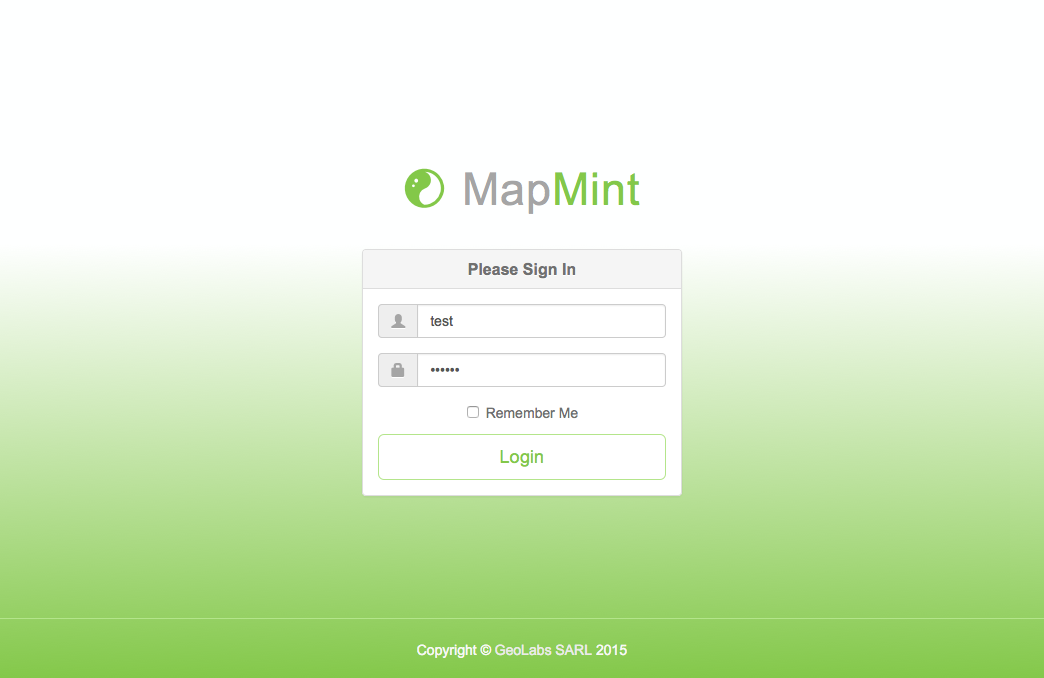
\includegraphics{login-screen.png}

A success message is displayed in a green frame on the top right of your screen and the module is charging. If you get a red banner at the top of the screen, please check your connection settings and try again.


\subsection{Access to the public interface}
\label{introduction/usemapmint:introduction-usemapmint-public-access}\label{introduction/usemapmint:acces-a-l-interface-publique}
The public interface of MapMint is accessible via the URL \href{http://votre-instance.com/public/}{http://votre-instance.com/public/} which is the home page of the application. The published cards are accessed from the Map Library (second menu tab). One can access an specific card using are specific URL (such \href{http://votre-instance.com/public/le-nom-de-votre-carte}{http://votre-instance.com/public/le-nom-de-votre-carte}).

\begin{tabulary}{\linewidth}{|L|L|}
\hline

\textbf{Module}
 & 
\textbf{URL access}
\\
\hline
Public interface
 & 
\href{http://votre-instance.com/public/}{http://votre-instance.com/public/}
\\
\hline
Public interface indicators
 & 
\href{http://votre-instance.com/public/indicateurs}{http://votre-instance.com/public/indicateurs}
\\
\hline
Published map
 & 
\href{http://votre-instance.com/public/le-nom-de-votre-carte}{http://votre-instance.com/public/le-nom-de-votre-carte}
\\
\hline\end{tabulary}



\subsection{First settings}
\label{introduction/usemapmint:premiers-parametrages}
During an initial connection, the following steps are recommended to ensure the proper functioning of the public interface.


\subsubsection{Title of the public interface}
\label{introduction/usemapmint:titre-de-l-interface-publique}
The title of the public interface appears in the banner at the top of the home page. To configure it, go to the {\hyperref[dashboard/configuration::doc]{\emph{\emph{Control Panel}}}} and change the value \textbf{Title} on the tab \emph{Provider Configuration}. Click the ``Save'' in the Control Panel and load your home page for the changes to take effect.

\begin{notice}{note}{Note:}
The title is also used in the \textless{}title\textgreater{} tag of the source code of the page
\end{notice}


\subsubsection{Map of the public interface}
\label{introduction/usemapmint:carte-de-l-interface-publique}
The public interface card appears in the body of the home page. To create and configure, go to the {\hyperref[maps/index::doc]{\emph{\emph{Map creation module}}}} and create a project named \textbf{Default}. Once registered, please reload this homepage for the map display.

\begin{notice}{note}{Note:}
Home card can be used to map a particular project that the user would like to see displayed on the home page. It can also be used as input to the different cartographic projects published. This requires the use of a data source that contains the URL of the projects.
\end{notice}


\subsection{Add data}
\label{introduction/usemapmint:ajouter-des-donnees}
Two solutions are proposed to charge GIS data on the installation server for your instance MapMint.

If you want to add light vector data ( \textbf{\textless{}2MB} ), go to the {\hyperref[data/index::doc]{\emph{\emph{Data Management Module}}}} and use the data load utility (upload), whose operation is described in the section on {\hyperref[data/index::doc]{\emph{\emph{Data Management Module}}}}.

If you want to load vector data or remain larger, you should use FTP access that was provided with the connection information to your instance MapMint. To do this, install and run a FTP client on your computer (such as \href{https://filezilla-project.org/}{FileZilla} for example) and provide the following information in the form provided for this purpose (the top of the software window in the case of FileZilla) and click the ``Login'' button.

\begin{tabulary}{\linewidth}{|L|L|}
\hline

\textbf{Parameter}
 & 
\textbf{Definition}
\\
\hline
Host
 & 
URL or IP address of the server where your instance is installed
\\
\hline
Username
 & 
Username provided by email
\\
\hline
Password
 & 
Password provided by email
\\
\hline\end{tabulary}


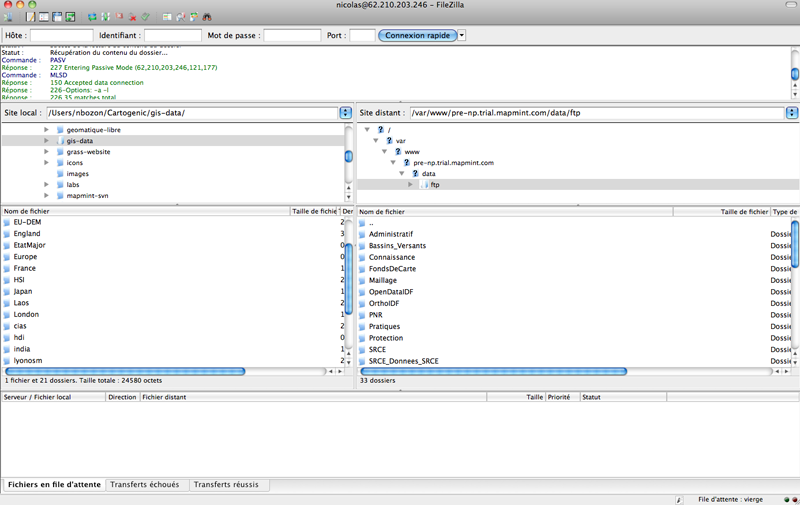
\includegraphics{upload-ftp.png}

Once connected to the server, the general repository for storing data sources (this is usually live in the /var/www/data/ftp) is listed and displayed in the FTP client the right window. You can then create a new folder or use an existing directory.
\begin{itemize}
\item {} 
In case you wish to add data to an existing directory, please perform drag and drop your data from the left side of the window (where the tree of your computer is listed) to the right, towards the directory referred. This causes the loading of data into the appropriate directory on the server. The progress of the file download is indicated by the progress bar at the bottom of the window. The transfer time varies depending on the weight of the data to be loaded.

\item {} 
In case you want to create a new folder, perform a right-click in the right pane and click the menu item ``Create New Folder'' from the popup menu that appears. Then enter a name for the new folder in the window provided for this purpose, then click the ``OK'' button. This will close the window and add the new directory to the list. You can then perform a drag and drop of your data as described in the preceding paragraph.

\end{itemize}

\begin{notice}{warning}{Warning:}
The name of a new data directory should not contain accents or special characters!
\end{notice}


\subsection{Access to data and processes from the desktop clients}
\label{introduction/usemapmint:acces-aux-donnees-et-traitements-depuis-des-clients-bureautiques}
As stated in the section {\hyperref[introduction/introduction:userguidegeneral]{\emph{Overview}}}, MapMint provided web services for accessing data (WMS, WFS and WCS) and data processing services (WPS) for desktop clients, such as  \href{http://www.qgis.org}{QGIS}.

We present in this section how to access them from QGIS data broadcasting services and data processing services. We will present successively as how to use them.


\subsubsection{Accessing data broadcasting services}
\label{introduction/usemapmint:acceder-aux-services-de-diffusion-de-donnees}
MapMint makes accessible all the storage spaces and sources of data that is printed once in the last parameters from the {\hyperref[maps/index:maps]{\emph{Map creation module}}}. Similarly, all the layers contained in the dynamic mapping applications configured for the {\hyperref[maps/index:maps]{\emph{Map creation module}}} and published since the {\hyperref[apps/index:apps]{\emph{Application Publishing Module}}} are also available.

Since QGIS for example, you can access the data layers in WMS format to keep the style you have defined at the {\hyperref[maps/index:maps]{\emph{Map creation module}}}, or format WFS, to use the data processing services vector.

The URL to use to set the access to WMS and WFS server are:
\begin{itemize}
\item {} 
for storage space \textless{}MyDirectory\textgreater{}:

\code{http://votre-instance.com/cgi-bin/mm/mapserver.cgi?map=/var/data/dirs/\textless{}MyDirectory\textgreater{}/ds\_ows.map}

\item {} 
for a project \textless{}MyProject\textgreater{} during setup:

\code{http://votre-instance.com/cgi-bin/mm/mapserver.cgi?map=/var/data/maps/project\_\textless{}MyProject\textgreater{}.map}

\item {} 
for a \textless{}MyProject\textgreater{} published project:

\code{http://votre-instance.com/cgi-bin/mm/mapserver.cgi?map=/var/data/public\_maps/project\_\textless{}MyProject\textgreater{}.map}

\end{itemize}

\begin{notice}{note}{Note:}
il est nécessaire de remplacer \code{\textless{}MyProject\textgreater{}} par le nom d'un projet et \code{\textless{}MyDirectory\textgreater{}} par le nom d'un espace de stockage disponible dans {\hyperref[data/index:data]{\emph{Data Management Module}}}.
\end{notice}

The two screenshots below shows the addition of WMS and WFS server.

\begin{tabulary}{\linewidth}{|L|L|}
\hline

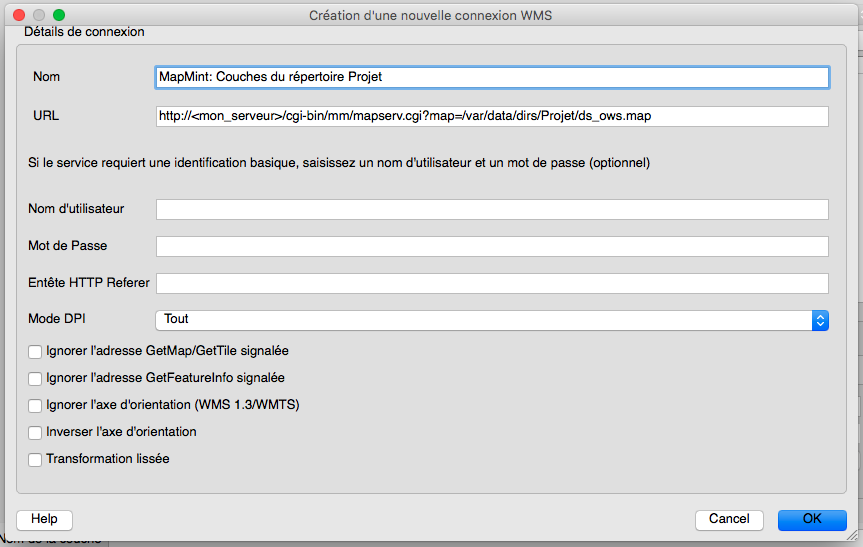
\includegraphics{qgis-wms.png}
 & 
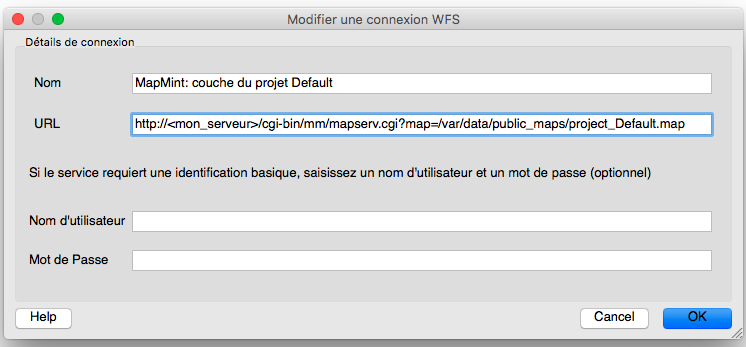
\includegraphics{qgis-wfs.png}
\\
\hline\end{tabulary}


Once you have added servers, then you can add layers in them. To do this, select vore server from the list of available servers, and then click \textbf{Connection} to list the available layers. Then select all the layers you want to display in your QGIS client.


\subsubsection{Access to data processing services}
\label{introduction/usemapmint:acceder-aux-services-de-traitements-de-donnees}
Since QGIS for example, you can access the vector data processing services. To do this it is necessary to add the following server \href{http://geolabs.fr/plugins.xml}{http://geolabs.fr/plugins.xml} your plugins DEPOS in QGIS, then install the module \textbf{QgsWPSClient}. Once this is done then you should enable this new extension, then add a WPS server (as was presented in the previous section for WMS and WFS service). Adding this fact via the interface shown in the screenshot below.

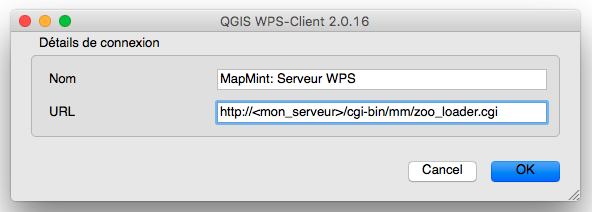
\includegraphics{qgis-wps.png}

The URL to access treatment services is:
\begin{quote}

\code{http://votre-instance.com/cgi-bin/mm/zoo\_loader.cgi}
\end{quote}

Once added the WPS server, select it in the list and click \textbf{Connect} to list the esemble of available treatment services as shown below.

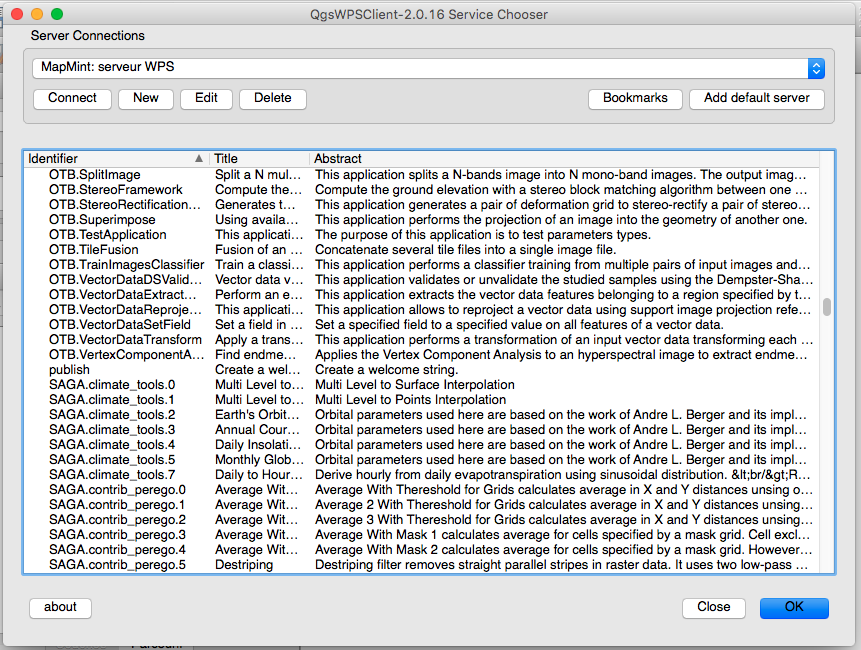
\includegraphics{qgis-wps-gc.png}

You must select a service was run by double-clicking on the service that interests you to access the through interface parameters WPS service. This interface corresponds to the following screenshot.

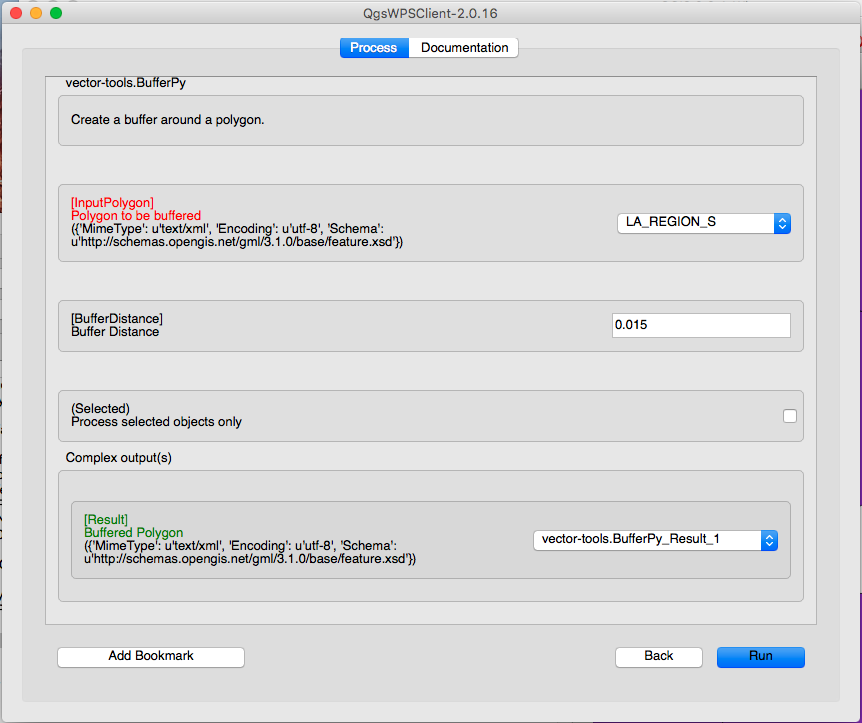
\includegraphics{qgis-wps-buff.png}

\begin{notice}{warning}{Warning:}
Only WFS and WCS layers can be used with WPS treatment services.
\end{notice}

To perform and display the result, you must click on the button \textbf{Run}.

We present below below an example of using a vector layer \textbf{LA\_REGION\_S} and execution services \textbf{vector-tools.BufferPy} et \textbf{vector-tools.CentroidPy}.

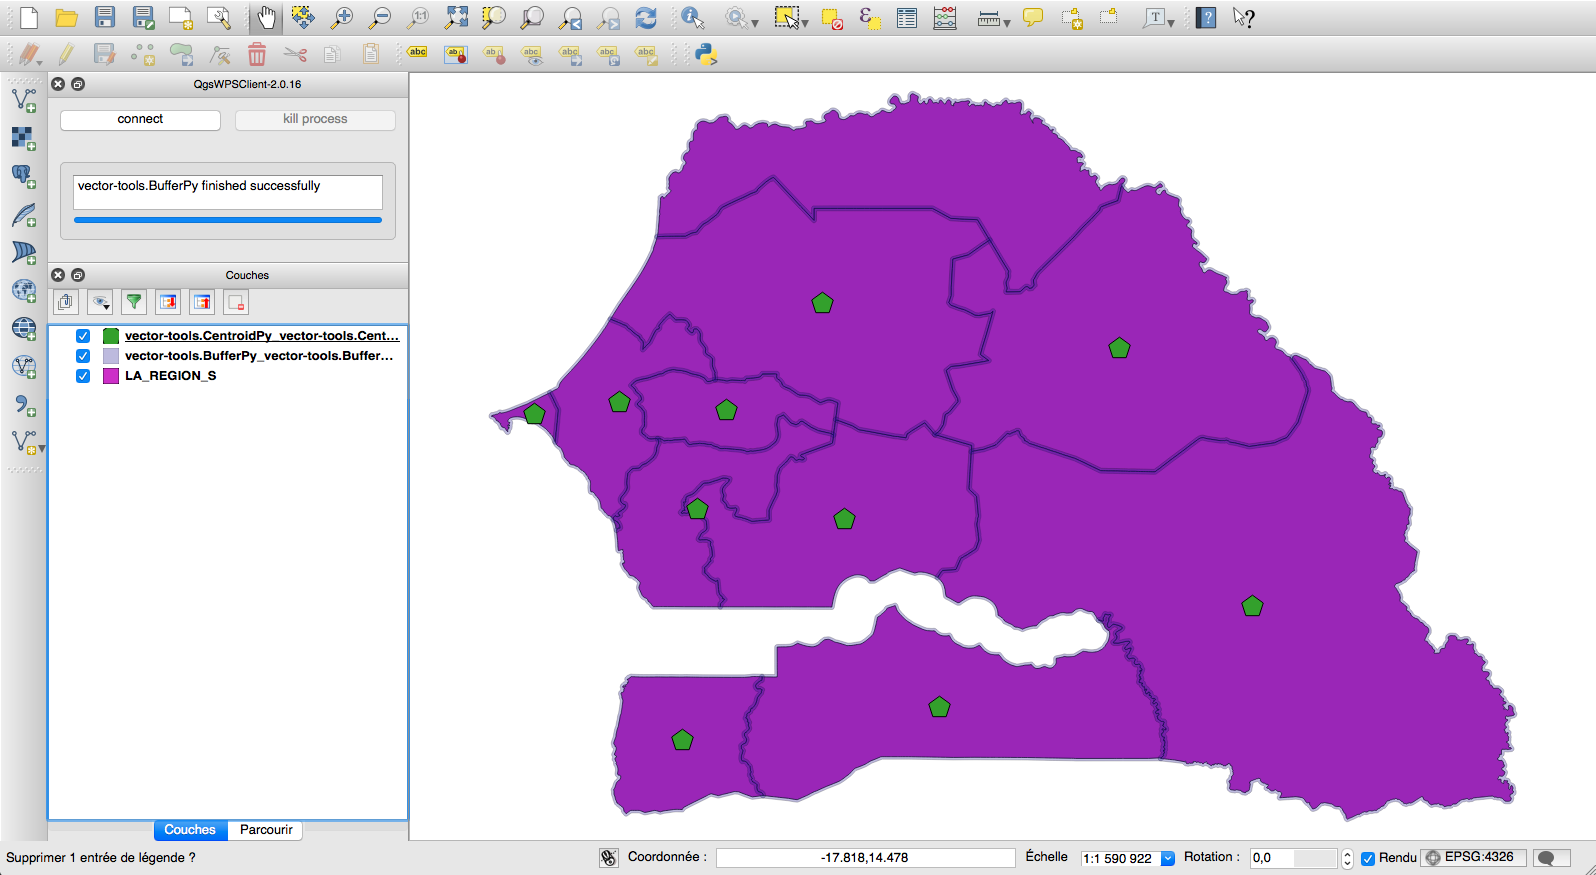
\includegraphics{qgis-wps-result.png}
..


\chapter{Dashboard}
\label{dashboard/index:tableau-de-bord}\label{dashboard/index::doc}\label{dashboard/index:dashboard}
This section contains the documentation for the dashboard MapMint.

The dashboard MapMint consists of three specific sections:
\begin{itemize}
\item {} 
\textbf{Overview} which is the visible content in page load,

\item {} 
\textbf{Users} that allows the management of users and user groups,

\item {} 
\textbf{Parameter} that allows the management of application settings.

\end{itemize}

\begin{notice}{warning}{Warning:}
It is important to note that only users in the group \textbf{super admin}  are allowed to access the modules {\hyperref[dashboard/usersmanagement:dashboard-usersmanagement]{\emph{User Management}}} and {\hyperref[dashboard/configuration:dashboard-configuration]{\emph{Control Panel}}}
\end{notice}


\section{Section ``Overview''}
\label{dashboard/overview::doc}\label{dashboard/overview:section-vue-d-ensemble}\label{dashboard/overview:dashboard-overview}
The panel ``Overview'' of the {\hyperref[dashboard/index::doc]{\emph{\emph{Dashboard}}}} provides an overview of the proceedings MapMint to a director of the application.

The date and time of your last connection to the proceeding are first shown at the top left.

Different panels have specific information about the MapMint instance, they are described in the following sections.

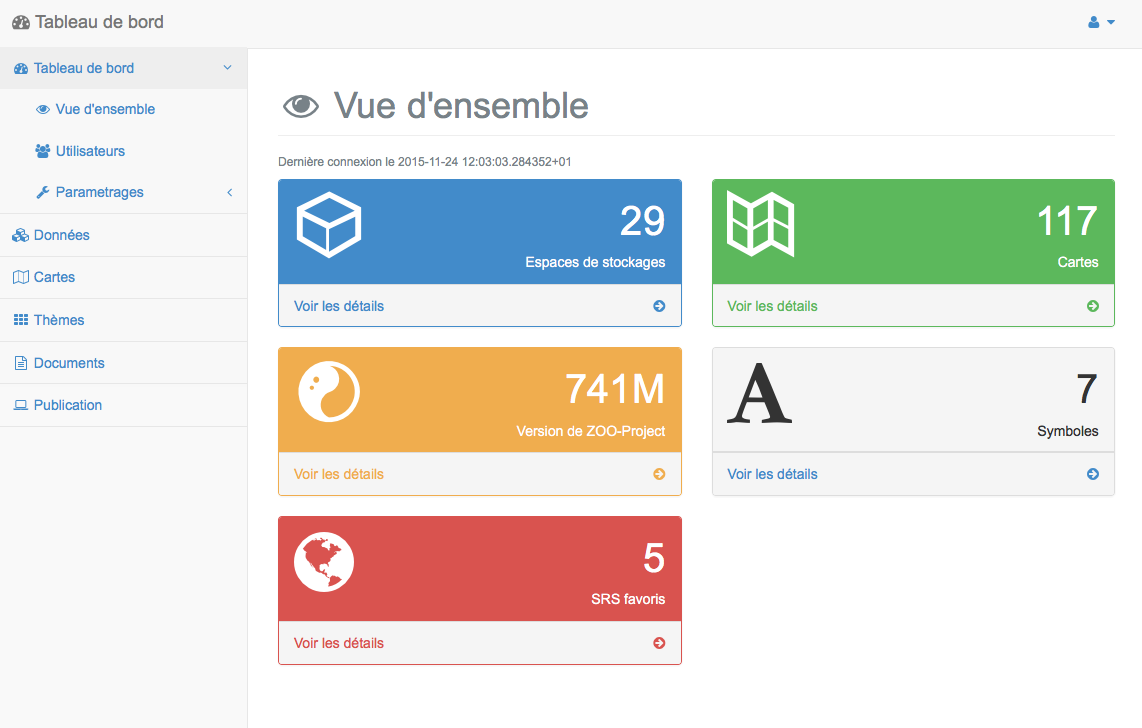
\includegraphics[width=1.000\linewidth]{dashboard-module-preview.png}


\subsection{Available data}
\label{dashboard/overview:donnees-disponibles}
Information relating to {\hyperref[data/index::doc]{\emph{\emph{Data Management Module}}}} are available in the blue panel shown below, it informs the administrator about:
\begin{itemize}
\item {} 
The number of new storage spaces

\item {} 
The number of directories and databases

\item {} 
The number of available data sources

\end{itemize}

A button allows you to go directly to {\hyperref[data/index::doc]{\emph{\emph{Data Management Module}}}}.

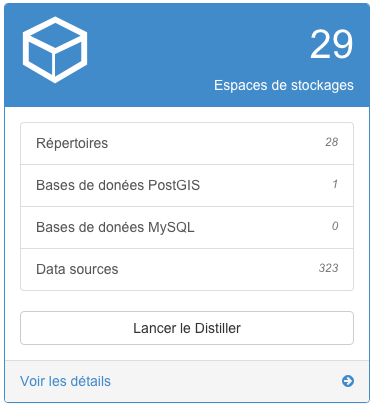
\includegraphics[width=0.330\linewidth]{dashboard-datastore-block.png}


\subsection{Cartes names available}
\label{dashboard/overview:nombres-de-cartes-disponibles}
Green panel shown below, provides a quick appercu of being edited cards. Clicking the pen of a card online, you can load the card in the {\hyperref[maps/index::doc]{\emph{\emph{Map creation module}}}}

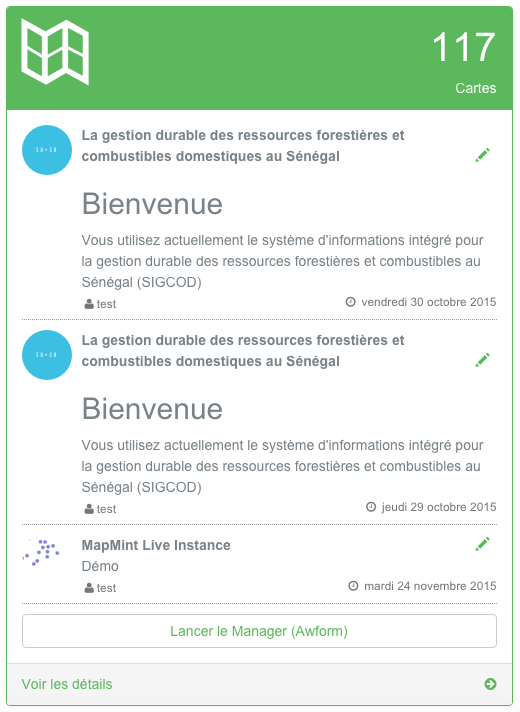
\includegraphics[width=0.330\linewidth]{dashboard-manager-block.png}


\subsection{Versions of installed software}
\label{dashboard/overview:versions-des-logiciels-installes}
The orange panel presented below, provides data on the versions of installed software and used by the MapMint application.

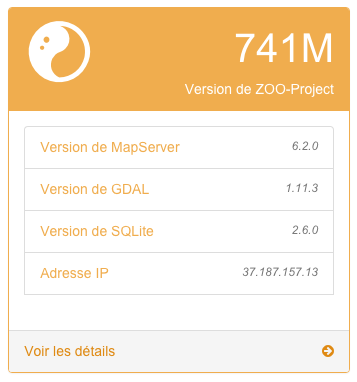
\includegraphics[width=0.330\linewidth]{dashboard-version-block.png}

This helps in problem report to specify the versions used.


\subsection{Symbol management}
\label{dashboard/overview:gestion-des-symboles}
The gray panel shown below list:
\begin{itemize}
\item {} 
the symbols that you can use to style your layers since the {\hyperref[data/index::doc]{\emph{\emph{Data Management Module}}}},

\item {} 
the fonts available in a dropdown list,

\item {} 
the list of symbols of a selected font.

\end{itemize}

It allows the management of symbols used to define the style of your layers. The procedure of this panel is very simple. If you select a font from this drop-down list in the middle of the panel, all of the symbols it contains will be displayed in desous. You can select Type single or multiple symbols in the list of symbols in a font and add them to the list of symbols available by clicking on the button ``+''. Similarly, you can select the symbols displayed above the drop-down list and click the ``-'' button to remove effectively.

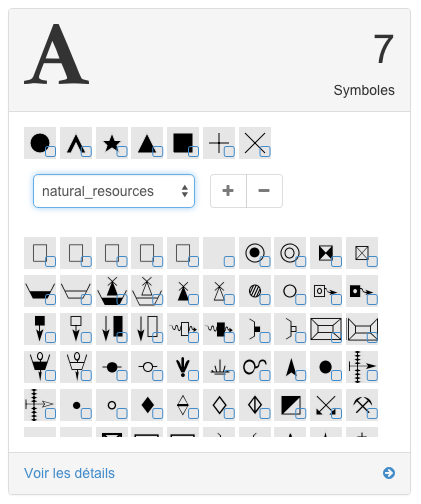
\includegraphics[width=0.330\linewidth]{dashboard-symbols-block.png}


\subsection{Management of Spatial Reference System (SRS)}
\label{dashboard/overview:gestion-des-systemes-de-references-spatiales-srs}
The red panel shows you the list of Spatial Reference System (SRS). If you enter or IGNF EPSG code in the box at the bottom of the panel, you can then add it to the list of favorites SRS. By clicking the ``trash'' button you can delete the SRS corresponding to the list of favorites. That is, unwanted in order to limit the number of SRS displayed in various forms in the application.

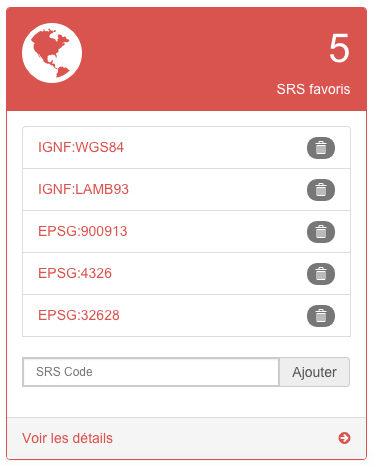
\includegraphics[width=0.330\linewidth]{dashboard-srs-block.png}


\section{User Management}
\label{dashboard/usersmanagement:gestion-des-utilisateurs}\label{dashboard/usersmanagement::doc}\label{dashboard/usersmanagement:dashboard-usersmanagement}
The User Management section lets you create, edit and delete users and user groups.

The page is divided into two tabs, ``Users'' and ``Groups''. Clicking on the title of the tab causes the display of the corresponding table.

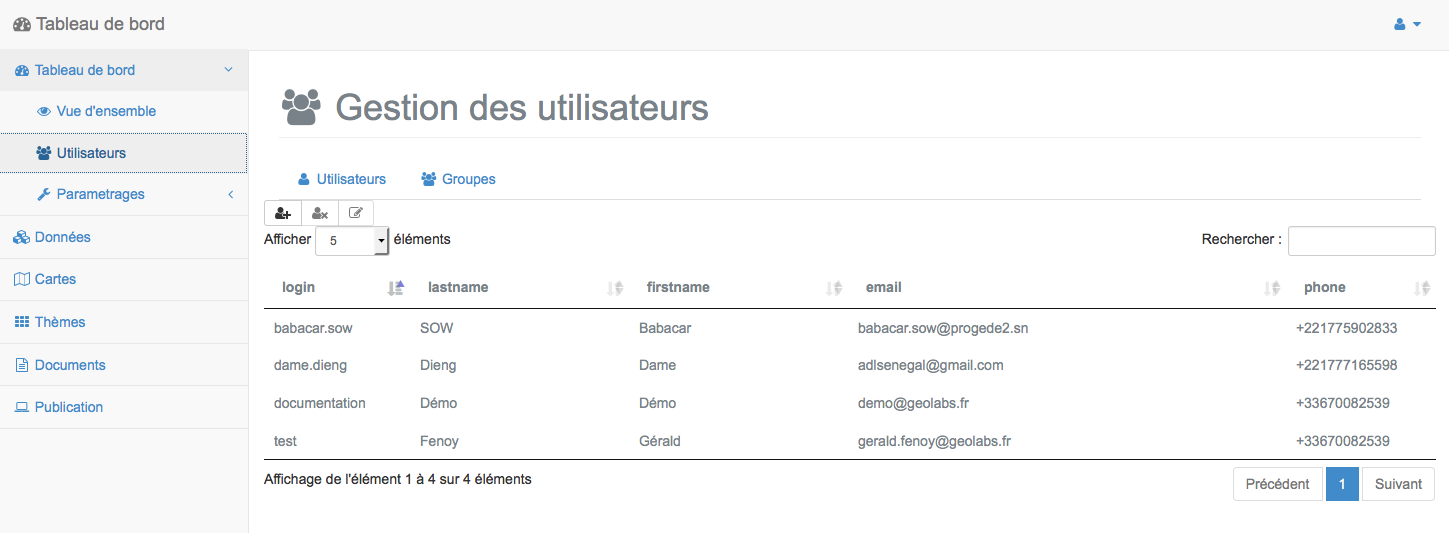
\includegraphics[width=1.000\linewidth]{manage-users-preview.png}

Each tab has the same toolbar having three buttons described below.

\begin{tabulary}{\linewidth}{|L|L|}
\hline

\textbf{Icon}
 & 
\textbf{Action}
\\
\hline

\includegraphics{add-user.png}
 & 
Displays the form to add a user / group
\\
\hline

\includegraphics{pencil.png}
 & 
Displays the edit form of a user / group
\\
\hline

\includegraphics{delete-user.png}
 & 
Displays the removal of a user form / Group
\\
\hline\end{tabulary}



\subsection{Add User}
\label{dashboard/usersmanagement:ajouter-un-utilisateur}
To add a new user, please click on the ``Add'' button on the left of the toolbar. This causes the display to add a user form. Please complete all fields and click on the ``Add'' button.

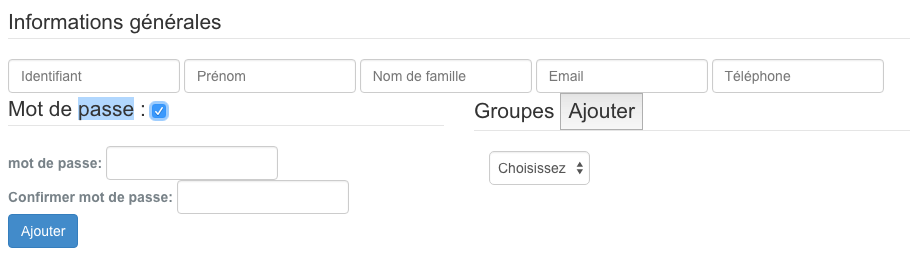
\includegraphics[width=1.000\linewidth]{dashboard-adduser-form.png}

\begin{tabulary}{\linewidth}{|L|L|}
\hline

\textbf{parameter}
 & 
\textbf{definition}
\\
\hline
Identification
 & 
Sets the user name for identification
\\
\hline
Name
 & 
Sets the name for the user profile
\\
\hline
First name
 & 
Sets the name of the user profile
\\
\hline
Password
 & 
Sets the password for identification
\\
\hline
email
 & 
Sets Electronic address of the user profile
\\
\hline
Phone
 & 
Specifies the user profile of the phone number
\\
\hline
Group
 & 
Sets / group(s) User
\\
\hline\end{tabulary}


\begin{notice}{warning}{Warning:}
All fields are required to create the user account.
\end{notice}

\begin{notice}{warning}{Warning:}
Check the rights necessary for the user and assign a group.
\end{notice}

\begin{notice}{note}{Note:}
The ``public'' is not connected to the user interface of the public.
\end{notice}

\begin{notice}{note}{Note:}
The phone supports the field type values +33100000000
\end{notice}


\subsection{Edit user}
\label{dashboard/usersmanagement:editer-un-utilisateur}
To edit a user click on a row in the user table. The latter is then highlighted (green color). Then click the ``Edit'' button to the toolbar, which causes the display of the edit form of the corresponding user.

All user settings are editable. Click the ``Save'' button to save the changes, which will be reported in a green band at the top of the screen.

\scalebox{0.800000}{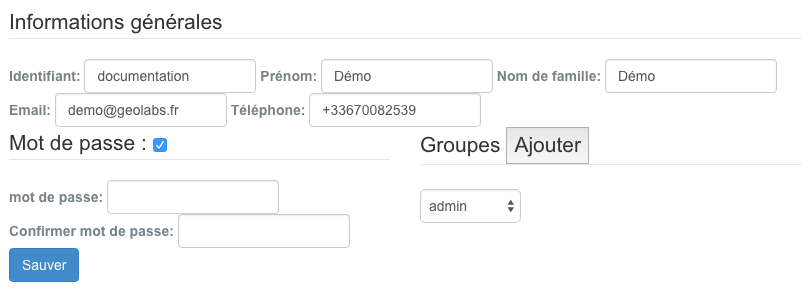
\includegraphics{edit-user-window.png}}

\begin{notice}{warning}{Warning:}
Changing the user group changes its rights
\end{notice}


\subsection{Delete User}
\label{dashboard/usersmanagement:supprimer-un-utilisateur}
To delete a user, click the corresponding line of the table and click the ``Remove'' button. This causes the display to delete a user form, shown below.

\scalebox{0.800000}{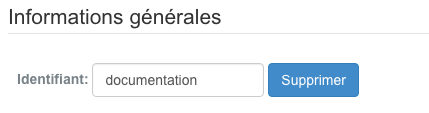
\includegraphics{delete-user-window.png}}

Click the ``Delete'' button to delete the user from the database.

\begin{notice}{warning}{Warning:}
Deleting a user is final!
\end{notice}


\subsection{Add Group}
\label{dashboard/usersmanagement:ajouter-un-groupe}
To create a new user group, please click on the tab ``Groups'' on top of the user management window, then click the ``Add'' button on the toolbar. This causes the display of the add form of a group, shown below.

\scalebox{0.800000}{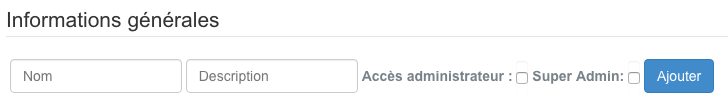
\includegraphics{add-usergroup-window.png}}

\begin{tabulary}{\linewidth}{|L|L|}
\hline

\textbf{Parameter}
 & 
\textbf{Definition}
\\
\hline
Name
 & 
Defines the group name
\\
\hline
Description
 & 
Defines the group with a short sentence
\\
\hline
Admin access
 & 
Defines whether the group has administrative access
\\
\hline
Super Admin
 & 
Defines if the group has a super administrator access
\\
\hline\end{tabulary}


Please complete all fields listed in the table above, then click on the ``Add'' button. This causes disparission form, adding the group in the table and then reload the page. Reopen the user management window and the ``Group'' tab to see the addition of the new group.

\begin{notice}{note}{Note:}
Adding users when creating the group is optional
\end{notice}

\begin{notice}{note}{Note:}
Groups with the  {\color{red}\bfseries{}**}Super Admin ** parameter checked are super administrators, so they have full access to the setup and user management.
\end{notice}


\subsection{Edit a group}
\label{dashboard/usersmanagement:editer-un-groupe}
To edit a group, click on a line in the corresponding table. The latter is then highlighted (blue color). Then click the ``Edit'' button to the toolbar, which causes the display of the edit form of the corresponding user group.

All group settings are editable. Click the ``Save'' button to save the changes.

\scalebox{0.800000}{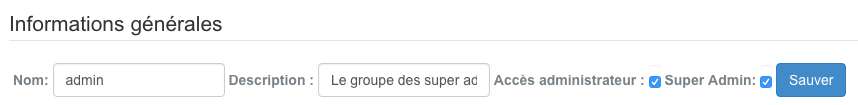
\includegraphics{edit-usergroup-window.png}}


\subsection{Remove Group}
\label{dashboard/usersmanagement:supprimer-un-groupe}
To delete a user group, click on the corresponding line of the table and click the ``Remove'' button. This causes the display to delete a user group form, as shown below.

\scalebox{0.800000}{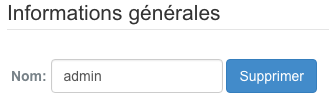
\includegraphics{delete-usergroup-window.png}}

The group name is specified in a text field, click the ``Remove'' button to remove the group. This causes the closure of the window, delete the group in the table and then reload the page.

\begin{notice}{warning}{Warning:}
Deleting a user group is final!
\end{notice}


\section{Control Panel}
\label{dashboard/configuration::doc}\label{dashboard/configuration:panneau-de-configuration}\label{dashboard/configuration:dashboard-configuration}
The control panel allows you to view and edit the installation settings of MapMint . Forms are automatically filled with the content of the \code{main.cfg} settings file .

\begin{notice}{warning}{Warning:}
It is not advisable to change the configuration settings without knowing the consequences
\end{notice}

The control panel is divided into 4 sections, listed below. Clicking on the icon causes the display of the tab.

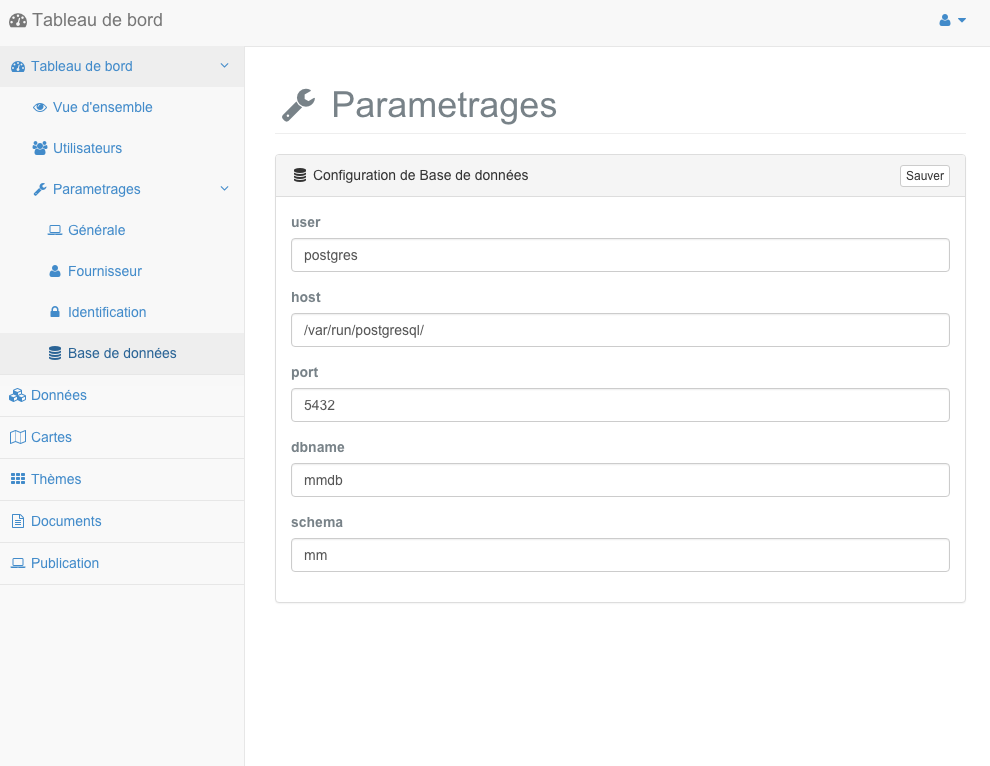
\includegraphics[width=1.000\linewidth]{dashboard-conf-form.png}

As presented in the previous screen, once you have edited the configuration settings, you to use the ``Save'' button at the top right of the panel to save your changes.

\begin{tabulary}{\linewidth}{|L|L|}
\hline

\textbf{Icon}
 & 
\textbf{Action}
\\
\hline

\includegraphics{monitor.png}
 & 
General configuration
\\
\hline

\includegraphics{security.png}
 & 
General configuration
\\
\hline

\includegraphics{user.png}
 & 
Provider Configuration
\\
\hline

\includegraphics{db.png}
 & 
Configuring the database
\\
\hline\end{tabulary}



\subsection{General configuration}
\label{dashboard/configuration:configuration-generale}
The general configuration form together the environment variables and installation parameters of the instance MapMint.

\begin{tabulary}{\linewidth}{|L|L|}
\hline

\textbf{Parameter}
 & 
\textbf{Definition}
\\
\hline
Encoding
 & 
Define the encoding of the default installation (utf-8)
\\
\hline
Mmadress
 & 
Set access to the default instance URL (/ mm /)
\\
\hline
Data path
 & 
Set path to the / data storage dedicated to data
\\
\hline
Jscache
 & 
Defines if the javascript files are compressed or not (prod \textbar{} dev)
\\
\hline
Tmp path
 & 
Sets the path to the temporary file storage directory (/ tmp /)
\\
\hline
Cache dir
 & 
Set path to the cache storage directory (/ cache /)
\\
\hline
3D
 & 
Sets the 3D Activation (false \textbar{} true)
\\
\hline
Root url
 & 
Set the URL to access the public interface by default (/ public /)
\\
\hline
publication Url
 & 
Set publishing URL where files are stored (/ public\_map /)
\\
\hline
Db link
 & 
Set path to the database instance users MapMint
\\
\hline
Mmpath
 & 
Set the full URL of the default installation directory (/ mm /)
\\
\hline
Version
 & 
Sets version number MapMint
\\
\hline
Rpy2
 & 
Sets the activation of the bookstore R (true \textbar{} false)
\\
\hline
Db user
 & 
Sets the name of the corresponding section in the parameters of the database
\\
\hline
Application adress
 & 
Sets the instance root address MapMint
\\
\hline
Lang
 & 
Defines the languages supported by the instance
\\
\hline
Sesspath
 & 
Set path to the session temporary files storage directory (/ tmp /)
\\
\hline
Publication path
 & 
Set path to the instance publishing directory MapMint
\\
\hline
Csscache
 & 
Defines whether the CSS files are compressed or not (prod \textbar{} dev)
\\
\hline
Msogcversion
 & 
Sets the version of the WMS and WFS services MapServer
\\
\hline
Server address
 & 
Set the URL to access the executable ZOO-Project (WPS kernel)
\\
\hline
Db username
 & 
Sets the name of the storage space corresponding to the user database
\\
\hline
Address templates
 & 
Set the URL to access the files models generated by the application (for windows and tooltips)
\\
\hline
Language
 & 
Sets the language of the proceedings
\\
\hline
Mapserveradress
 & 
Set the URL to access the executable MapServer
\\
\hline
Tmpurl
 & 
Set the access URL to the temporary directory (corresponding to the path tmp Path)
\\
\hline
templates Path
 & 
Defines the full path to the directory mapmint-ui / templates
\\
\hline\end{tabulary}



\subsection{General configuration}
\label{dashboard/configuration:configuration-de-l-identification}
configuration forms of ID and provider of services used to characterize the organization that publishes the data and the person responsible for the server and / or MapMint application.

\begin{tabulary}{\linewidth}{|L|L|}
\hline

\textbf{Parameter}
 & 
\textbf{Definition}
\\
\hline
Name position
 & 
Sets the position of the reference switch
\\
\hline
Individual Name
 & 
Sets the name of the individual reference contact
\\
\hline
Provide rname
 & 
Defines service provider name
\\
\hline
Administrative Area Address
 & 
Sets the administrative sector of the service provider
\\
\hline
Country address
 & 
Sets the service provider in the country
\\
\hline
Phone Voice
 & 
Sets the reference contact telephone number
\\
\hline
Address Postal Code
 & 
Sets the postal code of the service provider
\\
\hline
Role
 & 
Sets the service provider role
\\
\hline
Providersite
 & 
Sets the address of the service provider's website
\\
\hline
Phone Facsimile
 & 
Sets the fax number of the reference contract
\\
\hline
Address Electronic Mail Address
 & 
Sets the email address of the benchmark contract
\\
\hline
address City
 & 
Defines the city the service provider
\\
\hline
Delivery Point Address
 & 
Sets the service provider's address
\\
\hline\end{tabulary}


\begin{notice}{note}{Note:}
These parameters are used to define metadata ``open geospatial web services'' (OWS) defined by the Open Geospatial Consortium (OGC).
\end{notice}

\begin{notice}{note}{Note:}
The reference contact usually is the name of the person responsible for the server
\end{notice}


\subsection{Service Provider Configuration}
\label{dashboard/configuration:configuration-du-fournisseur-des-services}
\begin{tabulary}{\linewidth}{|L|L|}
\hline

\textbf{Parameter}
 & 
\textbf{Definition}
\\
\hline
Keywords
 & 
Sets keywords assigned to web services, separated by commas
\\
\hline
Title
 & 
Sets the title of the map server
\\
\hline
Abstract
 & 
Sets the map server with a short description
\\
\hline
Access Constraints
 & 
Defines if the map server requires authentication
\\
\hline
Fees
 & 
Defines the terms of use and / or the copyright server
\\
\hline\end{tabulary}


\begin{notice}{note}{Note:}
These parameters are used to define metadata ``open geospatial web services'' (OWS) defined by the Open Geospatial Consortium (OGC).
\end{notice}

\begin{notice}{note}{Note:}
The service provider usually is the name of the organization that publishes data
\end{notice}

\begin{notice}{warning}{Warning:}
The title and description of the server are also used in the home page of the public interface
\end{notice}


\subsection{Configuring the database}
\label{dashboard/configuration:configuration-de-la-base-de-donnees}
The Database Configuration page is only available when using a PostgreSQL type of database to store user information. In case you would use the SQLite database, this section should not appear.

\begin{tabulary}{\linewidth}{|L|L|}
\hline

\textbf{Parameter}
 & 
\textbf{Definition}
\\
\hline
user
 & 
Sets the user name to use to connect to the database server
\\
\hline
host
 & 
Sets the name of the machine or Unix domain socket used to connect to the database server
\\
\hline
port
 & 
Sets the port to use to connect to the database server
\\
\hline
dbname
 & 
Sets the name of the database to use
\\
\hline
schema
 & 
Sets the schema used for storing system tables
\\
\hline
password
 & 
Sets the password to use to connect to the database server
\\
\hline\end{tabulary}



\chapter{Territory management module}
\label{territories/index:territories}\label{territories/index::doc}\label{territories/index:module-de-gestion-des-territoires}
This section contains the documentation MapMint territories management module.

The territory management module manages a hierarchy of territories that will be subsequently used in the indicators management module to join a territory at a third data source (database query or other XLS, CSV. ..).

The page of the module is divided into two parts:
\begin{itemize}
\item {} 
the left side called the {\hyperref[territories/territorieslist::doc]{\emph{\emph{Panel territories}}}} it all territories created list and allows the addition and removal of territories

\item {} 
the right part called the {\hyperref[territories/infopanel::doc]{\emph{\emph{Information panel}}}} he used to enter the information at a document

\end{itemize}


\section{Panel territories}
\label{territories/territorieslist:territories-territorieslist}\label{territories/territorieslist:panneau-des-territoires}\label{territories/territorieslist::doc}
A territory consists of a name and a source of geographical data present in the PostGIS database of your instance MapMint. The territories are used as input parameters of the {\hyperref[indicators/index::doc]{\emph{\emph{Module creation indicators}}}}.
\setbox0\vbox{
\begin{minipage}{0.95\linewidth}
\textbf{Table of Contents}

\medskip

\begin{itemize}
\item {} 
\phantomsection\label{territories/territorieslist:id1}{\hyperref[territories/territorieslist:panneau-des-territoires]{\emph{Panel territories}}}
\begin{itemize}
\item {} 
\phantomsection\label{territories/territorieslist:id2}{\hyperref[territories/territorieslist:ajouter-un-nouveau-territoire]{\emph{Add a new territory}}}

\item {} 
\phantomsection\label{territories/territorieslist:id3}{\hyperref[territories/territorieslist:supprimer-un-territoire]{\emph{Delete territory}}}

\end{itemize}

\end{itemize}
\end{minipage}}
\begin{center}\setlength{\fboxsep}{5pt}\shadowbox{\box0}\end{center}

\begin{tabulary}{\linewidth}{|L|L|}
\hline

\textbf{Icon}
 & 
\textbf{Action}
\\
\hline

\includegraphics{add4.png}
 & 
Adds a new territory
\\
\hline

\includegraphics{delete5.png}
 & 
Removes territory
\\
\hline\end{tabulary}



\subsection{Add a new territory}
\label{territories/territorieslist:ajouter-un-nouveau-territoire}
To add a new area, click on the corresponding icon in the toolbar on the left panel. This shows the addition of territory form as shown below.

\scalebox{0.800000}{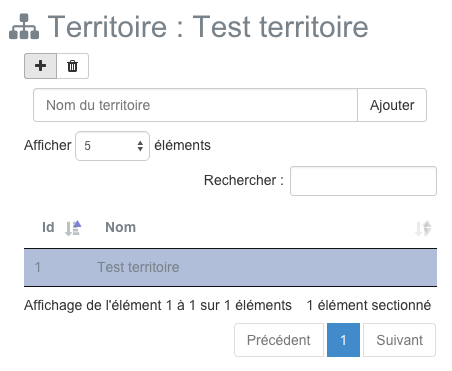
\includegraphics{add-territory-window.png}}

Please specify a name in the text box provided at this end and click on the ``Add'' button. This causes the form are gone, adding land to tree and reloading of the panel of {\hyperref[territories/infopanel::doc]{\emph{\emph{Information panel}}}}, to the right of the screen.


\subsection{Delete territory}
\label{territories/territorieslist:supprimer-un-territoire}
To remove an existing territory, please click on the name of the territory in the table, then on the icon to delete in the toolbar on the left panel. This displays the form of suppression of territory as shown below.

\scalebox{0.800000}{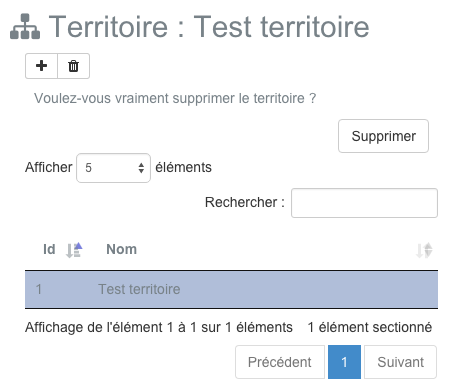
\includegraphics{delete-territory-window.png}}

Click the ``Delete'' button. This causes the form are gone and the removal of the tree area.

\begin{notice}{warning}{Warning:}
Deleting a territory is permanent and irreversible
\end{notice}


\section{Information panel}
\label{territories/infopanel::doc}\label{territories/infopanel:territories-infopanel}\label{territories/infopanel:panneau-d-information}\setbox0\vbox{
\begin{minipage}{0.95\linewidth}
\textbf{Table of Contents}

\medskip

\begin{itemize}
\item {} 
\phantomsection\label{territories/infopanel:id1}{\hyperref[territories/infopanel:panneau-d-information]{\emph{Information panel}}}
\begin{itemize}
\item {} 
\phantomsection\label{territories/infopanel:id2}{\hyperref[territories/infopanel:nom-du-territoire]{\emph{Territory Name}}}

\item {} 
\phantomsection\label{territories/infopanel:id3}{\hyperref[territories/infopanel:donnee-geographique]{\emph{Geographic Data}}}

\item {} 
\phantomsection\label{territories/infopanel:id4}{\hyperref[territories/infopanel:territoire-parent]{\emph{Parent territory}}}

\item {} 
\phantomsection\label{territories/infopanel:id5}{\hyperref[territories/infopanel:droits-des-groupes]{\emph{Rights groups}}}

\end{itemize}

\end{itemize}
\end{minipage}}
\begin{center}\setlength{\fboxsep}{5pt}\shadowbox{\box0}\end{center}

The territorial information panel lets you view and edit the properties of the territory selected following panel territories.

\scalebox{0.800000}{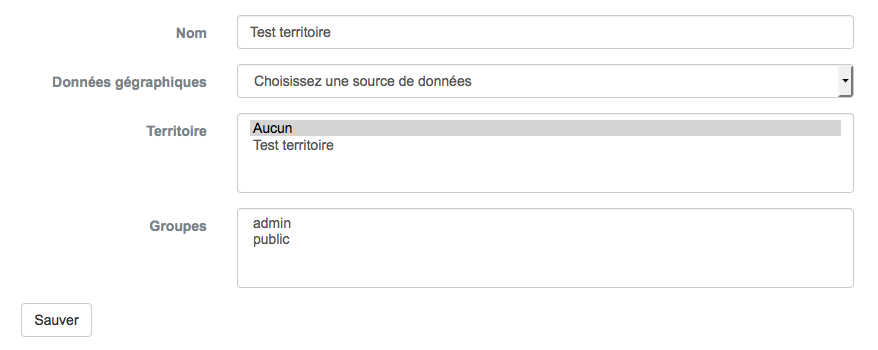
\includegraphics{territory-infopanel-window.png}}


\subsection{Territory Name}
\label{territories/infopanel:nom-du-territoire}
The name of the territory must be filled synthetic. The value of the text fields is used in the public interface.


\subsection{Geographic Data}
\label{territories/infopanel:donnee-geographique}
Select the database table that you want for the territory, using the drop-down list for this purpose.


\subsection{Parent territory}
\label{territories/infopanel:territoire-parent}
Select / parents territories with the multiple choice list for this purpose.


\subsection{Rights groups}
\label{territories/infopanel:droits-des-groupes}
The access to the territory may be restricted to certain user groups. Click on the / target groups in the multiple choice list for this purpose.

\begin{notice}{note}{Note:}
Click by holding down the Shift key to select multiple groups.
\end{notice}

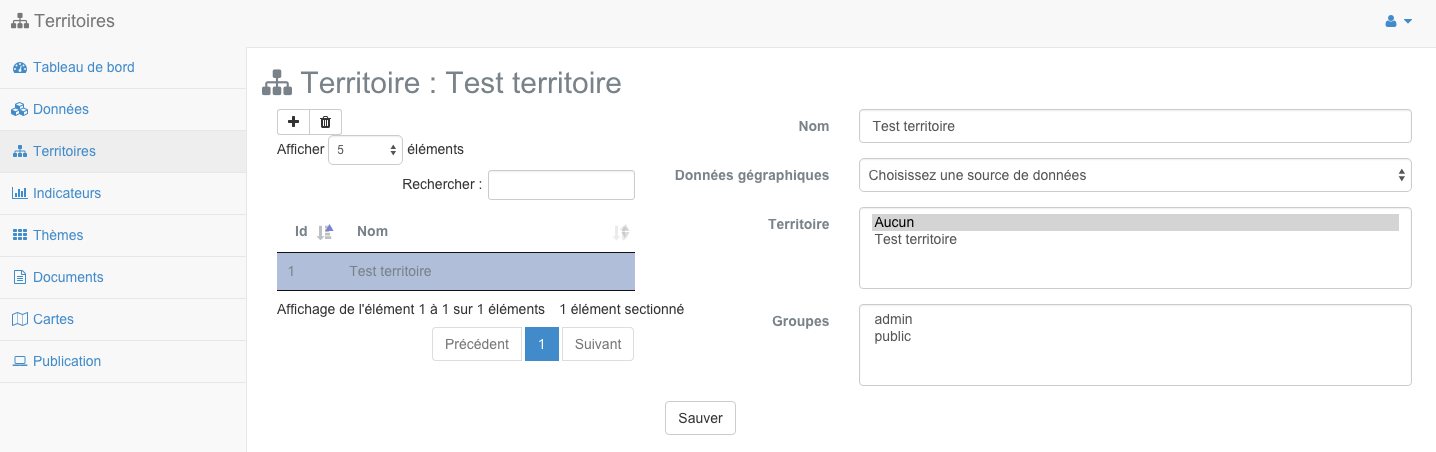
\includegraphics[width=1.000\linewidth]{territory-module-preview.png}


\chapter{Data Management Module}
\label{data/index:data}\label{data/index::doc}\label{data/index:module-de-gestion-des-donnees}
This section contains the documentation MapMint data management module.

MapMint uses abstraction library for access to geographic data \href{http://www.gdal.org}{GDAL} and the system is able to access similar to a database, a directory or data disseminated via the services of the \href{http://www.opengeospatial.org}{OGC} (WMS and WFS are currently supported). So MapMint defines the notion of \textbf{Data Stores} and \textbf{Data Sources}, where data store is a directory, a database or a server providing OGC web services and, a data source is a file in a directory, a geographic table of the database or a diffused layer available via OGC web service.


\section{Data Store}
\label{data/datastores:datadatastores}\label{data/datastores::doc}\label{data/datastores:espaces-de-stockage}\setbox0\vbox{
\begin{minipage}{0.95\linewidth}
\textbf{Table of Contents}

\medskip

\begin{itemize}
\item {} 
\phantomsection\label{data/datastores:id1}{\hyperref[data/datastores:espaces-de-stockage]{\emph{Data Store}}}
\begin{itemize}
\item {} 
\phantomsection\label{data/datastores:id2}{\hyperref[data/datastores:ajouter-un-espace-de-stockage]{\emph{Add storage space}}}
\begin{itemize}
\item {} 
\phantomsection\label{data/datastores:id3}{\hyperref[data/datastores:repertoires]{\emph{Directories}}}

\item {} 
\phantomsection\label{data/datastores:id4}{\hyperref[data/datastores:base-de-donnees]{\emph{Database}}}

\item {} 
\phantomsection\label{data/datastores:id5}{\hyperref[data/datastores:serveurs-ogc]{\emph{servers OGC}}}

\end{itemize}

\item {} 
\phantomsection\label{data/datastores:id6}{\hyperref[data/datastores:acceder-a-un-espace-de-stockage]{\emph{Access to storage space}}}
\begin{itemize}
\item {} 
\phantomsection\label{data/datastores:id7}{\hyperref[data/datastores:barre-d-outils-d-un-espace-de-stockage]{\emph{Toolbar of storage space}}}

\item {} 
\phantomsection\label{data/datastores:id8}{\hyperref[data/datastores:creer-une-mosaique-d-images]{\emph{Create a mosaic of images}}}

\item {} 
\phantomsection\label{data/datastores:id9}{\hyperref[data/datastores:envoyer-une-source-de-donnees-dans-un-espace-de-stockage]{\emph{Send a data source in a storage space}}}

\item {} 
\phantomsection\label{data/datastores:id10}{\hyperref[data/datastores:creer-un-index-de-tuiles-dans-un-espace-de-stockage]{\emph{Create a tile index in a storage space}}}

\item {} 
\phantomsection\label{data/datastores:id11}{\hyperref[data/datastores:gestion-des-droits-d-acces-d-un-espace-de-stockage]{\emph{Management of access rights to storage space}}}

\item {} 
\phantomsection\label{data/datastores:id12}{\hyperref[data/datastores:parametrage-d-un-espace-de-stockage]{\emph{Setting up storage space}}}

\item {} 
\phantomsection\label{data/datastores:id13}{\hyperref[data/datastores:supprimer-un-espace-de-stockage]{\emph{Remove storage space}}}

\item {} 
\phantomsection\label{data/datastores:id14}{\hyperref[data/datastores:rafraichir-un-espace-de-stockage]{\emph{Refresh storage space}}}

\end{itemize}

\end{itemize}

\end{itemize}
\end{minipage}}
\begin{center}\setlength{\fboxsep}{5pt}\shadowbox{\box0}\end{center}

A data store contains data sources, local or remote. It is defined by a name (without accents, spaces or special characters), as well as various parameters depending on its type. There are four types of storage space in MapMint:

\begin{tabulary}{\linewidth}{|L|L|L|}
\hline

\textbf{Icon}
 & 
\textbf{Type}
 & 
\textbf{Action}
\\
\hline

\includegraphics{database.png}
 & 
Database
 & 
Adding a connection to a database
\\
\hline

\includegraphics{directory.png}
 & 
repertoire
 & 
Adding a data directory
\\
\hline

\includegraphics{ogcserver.png}
 & 
Server OGC
 & 
Adding an external server OGC
\\
\hline\end{tabulary}


\begin{notice}{warning}{Warning:}
The name of a storage space must not contain any  \emph{space} \emph{emphasis}  \emph{or special characters}
\end{notice}


\subsection{Add storage space}
\label{data/datastores:ajouter-un-espace-de-stockage}\label{data/datastores:datadatastores-add}

\subsubsection{Directories}
\label{data/datastores:repertoires}
A directory type of storage allows for a symbolic link to an FTP server data directory. Click on the ``Add Directory'' found in the toolbar. This causes the display to add a directory form.

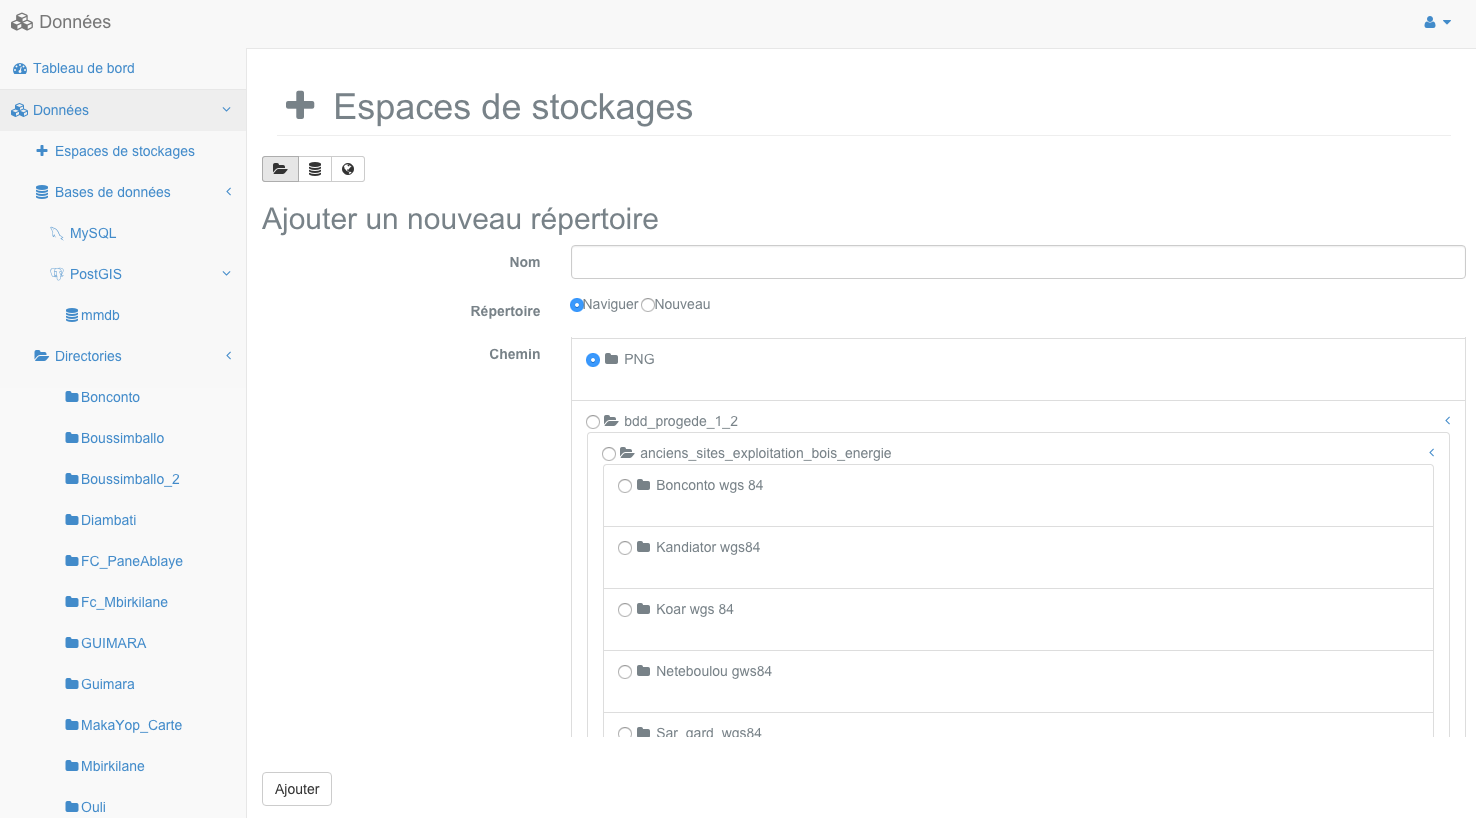
\includegraphics[width=1.000\linewidth]{add-directory-window.png}

Enter the name of the storage space and select a directory server in the directory tree (tree / data directory of the instance MapMint). You can create an empty folder on the FTP server by selecting the ``New'' option, then you must also name the directory to create.

\begin{notice}{warning}{Warning:}
The target directory does not contain sub directories.
\end{notice}

\begin{notice}{warning}{Warning:}
The target directory must contain only data formats supported by MapMint.
\end{notice}

This will close the window and the addition of new storage space in the left abre, in the Directories section.

\begin{notice}{note}{Note:}
Once the storage space created, make a right click on it and click ``Refresh''.
\end{notice}

Click on the storage space causes the display of data sources contained in the panel {\hyperref[data/datasources::doc]{\emph{\emph{Data Sources}}}}.


\subsubsection{Database}
\label{data/datastores:base-de-donnees}
A database type of storage enables a connection to a PostgreSQL or MySQL database. Click the ``Add Database'' icon in the top toolbar of the panel storage spaces. This causes the display to add a connection to form a database as shown below.

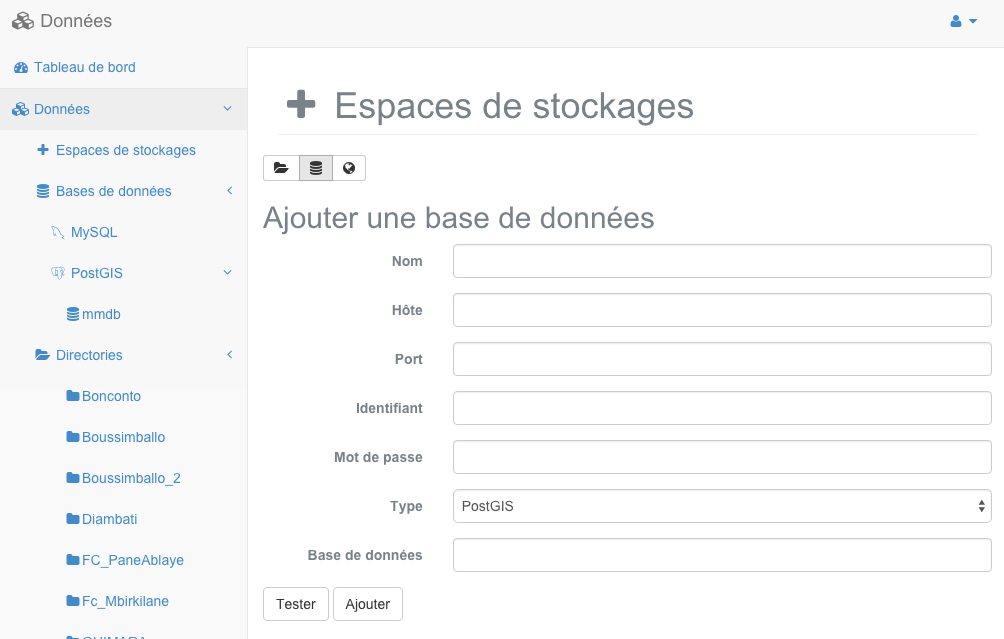
\includegraphics[width=1.000\linewidth]{add-database-window.png}

Complete all fields and click the ``Test'' button.

If the test returns a success message, you can then click on the ``Add'' button. This will close the window and the addition of new storage space in the left abre in the PostGIS or MySQL section.

\begin{notice}{note}{Note:}
Once the storage space created, click on it in the left menu to see the load is in the right side as shown in the previous screenshot.
\end{notice}

Click on the storage space causes its display in the right part.


\subsubsection{servers OGC}
\label{data/datastores:serveurs-ogc}
An OGC server-based storage enables a connection to a server or external WMS WFS. Click on the ``Add a server OGC'' found in the toolbar, this causes the display of the add form of OGC server.

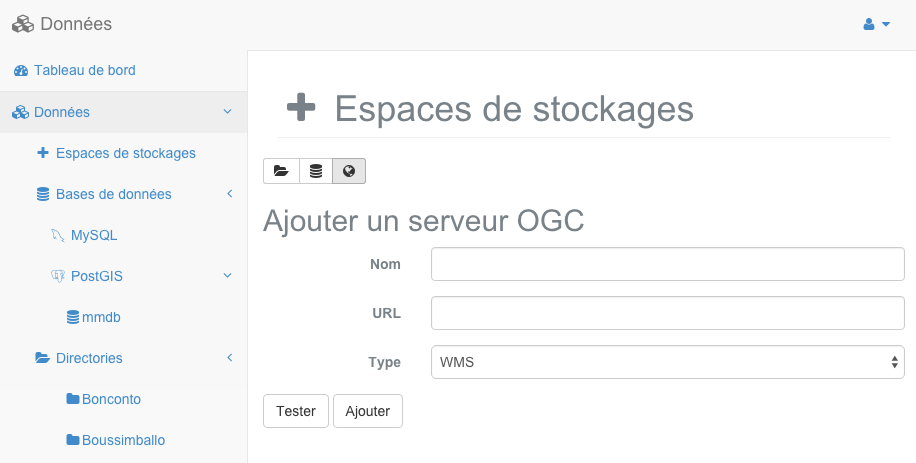
\includegraphics[width=1.000\linewidth]{add-ogcserver-window.png}

Enter the name of the storage space, target OGC server URL and protocol to use (WMS or WFS), and click the ``Test'' button.

If the test returns a success message, you can then click on the ``Add'' button. This will close the window and the addition of new storage space in the left tree in the WFS Server section.

Click on the storage space causes the display of OGC layers of the external server.


\subsection{Access to storage space}
\label{data/datastores:acceder-a-un-espace-de-stockage}
When you click on the storage space that causes its display as illstré below.

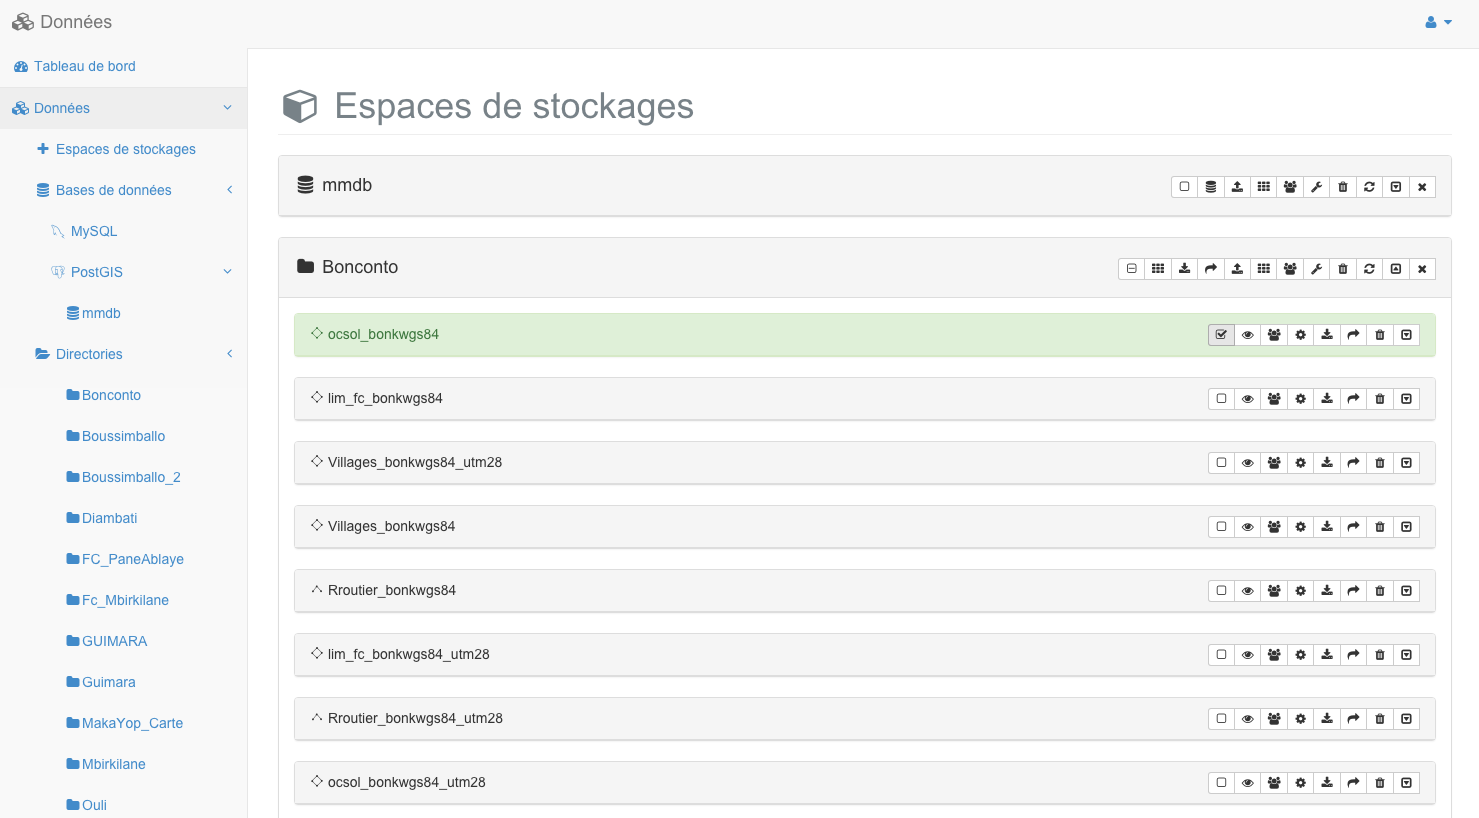
\includegraphics[width=1.000\linewidth]{data-store-preview.png}

Storage spaces offer specific functions according to their type, all buttons on the toolbar for a stockagre space is presented below. For each button, the type of storage from which the function is accessible also highlighted.


\subsubsection{Toolbar of storage space}
\label{data/datastores:barre-d-outils-d-un-espace-de-stockage}
\begin{tabulary}{\linewidth}{|L|L|L|}
\hline

\textbf{Icon}
 & 
\textbf{Accessible}
 & 
\textbf{Action}
\\
\hline

\includegraphics{select.png}
 & 
All
 & 
Select all the contained data sources
\\
\hline

\includegraphics{tile.png}
 & 
repertoire
 & 
Create a mosaic of images (requires a data source selected image)
\\
\hline

\includegraphics{download.png}
 & 
repertoire
 & 
Download the selected data sources (requires a data source selected image)
\\
\hline

\includegraphics{share.png}
 & 
All
 & 
Open data sources selectionnées in {\hyperref[maps/index:maps]{\emph{Map creation module}}} (requires selected data source)
\\
\hline
\includegraphics{database.png}
 & 
Database
 & 
Access to the database
\\
\hline
\includegraphics{upload.png}
 & 
repertoire
 & 
Send a data source in the server storage space
\\
\hline
\includegraphics{tile.png}
 & 
repertoire
 & 
Creating a tile index in the storage space
\\
\hline
\includegraphics{privileges.png}
 & 
all
 & 
Management of access rights to storage space
\\
\hline
\includegraphics{configuration.png}
 & 
all
 & 
Setting the storage space
\\
\hline
\includegraphics{delete.png}
 & 
All
 & 
Remove the storage space
\\
\hline
\includegraphics{refresh.png}
 & 
All
 & 
Refresh the storage space
\\
\hline
\includegraphics{toggle1.png}
 & 
All
 & 
Show / hide storage space
\\
\hline
\includegraphics{close.png}
 & 
All
 & 
Close the storage space
\\
\hline\end{tabulary}



\subsubsection{Create a mosaic of images}
\label{data/datastores:creer-une-mosaique-d-images}
Creating a mosaic of images allows merging several images data sources into one.

When you click on ``Create an image mosaic'' button the form presented below desous appears. Once you have entered the name of the mosaic to create, click the ``Mosaic'' button to generate it.

\begin{notice}{warning}{Warning:}
This may take time depending on the selected image data sources.
\end{notice}

\includegraphics[width=1.000\linewidth]{data-store-mozaic.png}


\subsubsection{Send a data source in a storage space}
\label{data/datastores:envoyer-une-source-de-donnees-dans-un-espace-de-stockage}
You can use the panel a storage space for to send a geographical data file you have on your local machine. This is done using the form provided below.

You can then click on the ``Browse'' button to add files to the list of files to send.

\begin{notice}{warning}{Warning:}
While sending data sources feature available on MapMint platform, it should only be used for data sources does not exceed 10MB.
\end{notice}

\includegraphics[width=1.000\linewidth]{data-store-upload.png}


\subsubsection{Create a tile index in a storage space}
\label{data/datastores:creer-un-index-de-tuiles-dans-un-espace-de-stockage}
When it is desired to publish data sources aerial photograph-like images for example, it is necessary to use a tile index. A tile index is a source of data vectors (type polygon) where each polygon represents the geographical area covered by an image data source (aerial photographs, for example) and one property that is the full path to the image file .

To create a tile index, you must place a directory containing all the images with which you want to create a tile index. Once done, you can click on the button ``Create a tile index'' of the storage space in which to store it, the form shown below appears. Select the SRS index to create, enter the file extension to use (eg tif) and select the folder storing your photos, click on the button ``tile Index'' to generate the tile index.

\includegraphics[width=1.000\linewidth]{data-tileindex.png}


\subsubsection{Management of access rights to storage space}
\label{data/datastores:gestion-des-droits-d-acces-d-un-espace-de-stockage}
A data source is accessible to all user groups by default. To change the permissions to access a layer, click on the corresponding icon in the {\hyperref[data/datasources:datasource-table-label]{\emph{Bar Data source tools}}}. This prompts the access rights management form shown below.

\includegraphics[width=1.000\linewidth]{data-privileges.png}

The rights that you can assign to a user group are listed in the following table.

\begin{tabulary}{\linewidth}{|L|L|}
\hline

\textbf{Value}
 & 
\textbf{Definition}
\\
\hline
r
 & 
The access to user group to read the storage space
\\
\hline
w
 & 
The group of users to access the write storage
\\
\hline
x
 & 
The user group has the right to run services in the storage space
\\
\hline\end{tabulary}


Add Type single or multiple groups with the ``Add'' button, this entails adding drop-down lists in the window. Adjust the values  \textbf{r}, \textbf{w}  and  \textbf{x} and then click the ``Submit'' button. The form disappears and recording changes is achieved.

If you click the ``Delete'' button you can delete the last line of setting access privileges.

To see the right to list the contents of a storage space a user group must have the rights \textbf{r} and \textbf{x}. To create new sources of data in the storage space, a group must have the right \textbf{w}.


\subsubsection{Setting up storage space}
\label{data/datastores:parametrage-d-un-espace-de-stockage}
The settings form a storage space and the equivalent of adding specific form to the type of storage space seen {\hyperref[data/datastores:datadatastores-add]{\emph{previously}}}.


\subsubsection{Remove storage space}
\label{data/datastores:supprimer-un-espace-de-stockage}
If you click on the button ``Remove storage'', a window appears asking you to confirm your desire to remove a storage space. Deleting a storage space can cause serious data loss and involve the largest public application becomes unstable due to the unavailability of necessary data sources. It is therefore imperative to ensure that no project depends on data in the storage space you want to remove before making the. If you really want to delete a storage space, then click the ``Yes'' button in the window informing you of the implications of the removal.


\subsubsection{Refresh storage space}
\label{data/datastores:rafraichir-un-espace-de-stockage}
On first access to storage space, creates a specific MapMint Mapfile MapServer allows the distribution of the contained data sources. Once this file is created, it is not changed. This means that if you have added, deleted or created a new source of data storage space, you should use the refresh button to obtain a comprehensive list of data sources contained in a storage space. When you click the refresh button, the contents of the storage space is updated.


\section{Data Sources}
\label{data/datasources:data-datasources}\label{data/datasources::doc}\label{data/datasources:sources-de-donnees}\setbox0\vbox{
\begin{minipage}{0.95\linewidth}
\textbf{Table of Contents}

\medskip

\begin{itemize}
\item {} 
\phantomsection\label{data/datasources:id6}{\hyperref[data/datasources:sources-de-donnees]{\emph{Data Sources}}}
\begin{itemize}
\item {} 
\phantomsection\label{data/datasources:id7}{\hyperref[data/datasources:donnees-vectorielles]{\emph{vector data}}}
\begin{itemize}
\item {} 
\phantomsection\label{data/datasources:id8}{\hyperref[data/datasources:formats-supportes]{\emph{supported formats}}}

\item {} 
\phantomsection\label{data/datasources:id9}{\hyperref[data/datasources:consulter-la-table]{\emph{Refer to the table}}}

\item {} 
\phantomsection\label{data/datasources:id10}{\hyperref[data/datasources:definir-l-encodage-des-caracteres-de-la-table]{\emph{Define the encoding of the character table}}}

\end{itemize}

\item {} 
\phantomsection\label{data/datasources:id11}{\hyperref[data/datasources:donnees-matricielles]{\emph{raster data}}}
\begin{itemize}
\item {} 
\phantomsection\label{data/datasources:id12}{\hyperref[data/datasources:id1]{\emph{supported formats}}}

\item {} 
\phantomsection\label{data/datasources:id13}{\hyperref[data/datasources:consulter-l-histogramme]{\emph{Look at the histogram}}}

\end{itemize}

\item {} 
\phantomsection\label{data/datasources:id14}{\hyperref[data/datasources:barre-d-outils-des-sources-de-donnees]{\emph{Bar Data source tools}}}
\begin{itemize}
\item {} 
\phantomsection\label{data/datasources:id15}{\hyperref[data/datasources:droits-d-acces]{\emph{Access rights}}}

\item {} 
\phantomsection\label{data/datasources:id16}{\hyperref[data/datasources:convertir-une-source-de-donnees]{\emph{Convert a data source}}}

\item {} 
\phantomsection\label{data/datasources:id17}{\hyperref[data/datasources:telechargement]{\emph{Downloading}}}

\item {} 
\phantomsection\label{data/datasources:id18}{\hyperref[data/datasources:previsualisation]{\emph{preview}}}

\item {} 
\phantomsection\label{data/datasources:id19}{\hyperref[data/datasources:suppression]{\emph{Removal}}}

\item {} 
\phantomsection\label{data/datasources:id20}{\hyperref[data/datasources:ouverture]{\emph{Opening}}}

\end{itemize}

\end{itemize}

\end{itemize}
\end{minipage}}
\begin{center}\setlength{\fboxsep}{5pt}\shadowbox{\box0}\end{center}

A data source consists of one or more spatially referenced information contained by one of the {\hyperref[data/datastores::doc]{\emph{\emph{Data Store}}}} available. MapMint supports several types of data sources in this section.

The pictograms used to illustrate the type of data source are shown in the following table.

\begin{tabulary}{\linewidth}{|L|L|}
\hline

\textbf{Icon}
 & 
\textbf{Type}
\\
\hline
\includegraphics{data-vector-point-icon.png}
 & 
Point Vector Data Source
\\
\hline
\includegraphics{data-vector-line-icon.png}
 & 
Line Vector Data Source
\\
\hline
\includegraphics{data-vector-polygon-icon.png}
 & 
Vector Polygon Data Source
\\
\hline
\includegraphics{data-raster-icon.png}
 & 
Raster data source
\\
\hline\end{tabulary}



\subsection{vector data}
\label{data/datasources:donnees-vectorielles}

\subsubsection{supported formats}
\label{data/datasources:formats-supportes}
MapMint supports vector data formats listed below.

\begin{tabulary}{\linewidth}{|L|L|L|}
\hline

\textbf{Format}
 & 
\textbf{Code}
 & 
** Required  Files**
\\
\hline
Comma Separated Value
 & 
CSV
 & 
csv
\\
\hline
ESRI Shapefile
 & 
SHP
 & 
shp,dbf,shx,prj
\\
\hline
GPX
 & 
GPX
 & 
gpx
\\
\hline
Mapinfo
 & 
MIF
 & 
mif
\\
\hline
KML
 & 
KML
 & 
kml
\\
\hline
PostgreSQL/PostGIS
 & 
PostGIS
 & 
connection PostGIS
\\
\hline
Web Feature Service
 & 
WFS
 & 
connection WFS
\\
\hline\end{tabulary}


\begin{notice}{note}{Note:}
\emph{Other formats \textless{}http://www.gdal.org/ogr/ogr\_formats.html\textgreater{}} \_\_ supported by the  \emph{OGR \textless{}http://www.gdal.org/ogr\textgreater{}} library \_\_ can also be used with MapMint.
\end{notice}


\subsubsection{Refer to the table}
\label{data/datasources:consulter-la-table}
For a table of a data source, click on the ``arrow'' icon to the right of the: ref: \emph{datasource-table-label}. This causes the éffichage of the data table. An example of this table is presented below.

{\color{red}\bfseries{}\textbar{}view\textbar{}}

Once the displayed table, and if it contains a sufficient number of entities, it is possible to navigate through the different pages of the table using the buttons ``Previous'' and ``Next'' displayed on the bottom navigation the table or by clicking directly on the number of the desired page.

In case the contents of the corresponding table in your data source is not displayed correctly, refer to the section: ref: \emph{data-datasource-encoding}. then you must define the encoding of your data source, using the text fields provided for this purpose and clicking the ``Set'' button.

\begin{notice}{note}{Note:}
The dropdown list at the top left of the table allows you to display 10, 15, 20, 25 or 30 units per page
\end{notice}

\begin{notice}{note}{Note:}
Clicking on a title of a column to sort the values in ascending / descending order or alphabetically.
\end{notice}


\subsubsection{Define the encoding of the character table}
\label{data/datasources:definir-l-encodage-des-caracteres-de-la-table}
MapMint use UTF-8 encoding to display the default data source tables. However, it is common for data encoded in a different system to be loaded into the data management module. In this case, it is possible to assign a different encoding system in the text fields provided for this purpose, the right of the navigation bar.

Please enter the code of the desired encoding and click on the ``Refresh'' from the toolbar. This results in reloading the table and its display in the desired encoding.

Examples of character encoding are listed below for your information:

\begin{tabulary}{\linewidth}{|L|L|}
\hline

\textbf{Code}
 & 
\textbf{Description}
\\
\hline
utf-8
 & 
All Unicode international character has ASCII-compatible (English)
\\
\hline
iso-8859-1
 & 
Latin alphabet No. 1 containing 191 characters of the Latin alphabet
\\
\hline
iscii
 & 
Alphasyllabaire used in India, Sri Lanka and Bangladesh
\\
\hline
viscii
 & 
Vietnamese modern Latin alphabet
\\
\hline
shift-jis
 & 
Syllabary writing scenic and traditional Japanese languages
\\
\hline\end{tabulary}


\begin{notice}{note}{Note:}
Get more information about the character encoding of \href{http://fr.wikipedia.org/wiki/Codage\_des\_caract\%C3\%A8res}{Wikipedia}
\end{notice}


\subsection{raster data}
\label{data/datasources:donnees-matricielles}

\subsubsection{supported formats}
\label{data/datasources:id1}
MapMint supports raster data formats listed below.

\begin{tabulary}{\linewidth}{|L|L|L|}
\hline

\textbf{Format}
 & 
\textbf{Code}
 & 
** Required  Files**
\\
\hline
Arc/Info ASCII Grid
 & 
AAIGrid
 & 
asc
\\
\hline
GeoTiff
 & 
GTiff
 & 
tif
\\
\hline
JPEG
 & 
JPEG
 & 
jpg
\\
\hline\end{tabulary}


\begin{notice}{note}{Note:}
Oher formats {}` \textless{}\href{http://www.gdal.org/formats\_list.html}{http://www.gdal.org/formats\_list.html}\textgreater{}{}`\_\_ Supported by the \href{http://www.gdal.org}{GDAL} can also be used with MapMint.
\end{notice}


\subsubsection{Look at the histogram}
\label{data/datasources:consulter-l-histogramme}
To view the histogram of a data source, click on the ``arrow'' icon to the right of the: ref: \emph{datasource-table-label}. This causes unfolding of the histogram, as illustrated below.

{\color{red}\bfseries{}\textbar{}view\textbar{}}

The histogram of the data source allows you to view the distribution in the pixel array.

\begin{notice}{note}{Note:}
It is possible to zoom in the histogram by holding your cursor and a drawing a rectangle.
\end{notice}


\subsection{Bar Data source tools}
\label{data/datasources:barre-d-outils-des-sources-de-donnees}\label{data/datasources:datasource-table-label}
\begin{tabulary}{\linewidth}{|L|L|}
\hline

\textbf{Icon}
 & 
\textbf{Action}
\\
\hline
\includegraphics{privileges.png}
 & 
Set access permissions for a data source
\\
\hline
\includegraphics{process1.png}
 & 
Convert a data source
\\
\hline
\includegraphics{download.png}
 & 
Download a data source
\\
\hline
\includegraphics{preview.png}
 & 
Preview a Data Source
\\
\hline
\includegraphics{share.png}
 & 
Open a data source in the card creation module
\\
\hline
\includegraphics{delete.png}
 & 
Delete a data source
\\
\hline\end{tabulary}



\subsubsection{Access rights}
\label{data/datasources:droits-d-acces}
A data source is accessible to all user groups by default. To change the permissions to access a layer, click on the corresponding icon in the: ref: \emph{datasource-table-label}. This will open the window of access rights, as shown below:

\includegraphics[width=1.000\linewidth]{data-privileges.png}

\begin{tabulary}{\linewidth}{|L|L|}
\hline

\textbf{Value}
 & 
\textbf{Definition}
\\
\hline
r
 & 
The user group access to reading in bed
\\
\hline
w
 & 
The user group to access the write layer
\\
\hline
x
 & 
The user group to access ...
\\
\hline\end{tabulary}


Add Type single or multiple groups with the ``Add'' button, this entails adding drop-down lists in the window. Adjust the values  {\color{red}\bfseries{}**}r ** {\color{red}\bfseries{}**}w **  and  {\color{red}\bfseries{}**}x ** and then click the ``Submit'' button. The window closes and recording changes is stated at the top of your screen in a green headband.


\subsubsection{Convert a data source}
\label{data/datasources:convertir-une-source-de-donnees}
Data conversion is covered in part:: ref: \emph{data-processing}.


\subsubsection{Downloading}
\label{data/datasources:telechargement}
To download a data source on your computer, just click on the corresponding icon in the: ref: \emph{datasource-table-label}. This causes the direct download of the data, stored in a .zip file


\subsubsection{preview}
\label{data/datasources:previsualisation}
To preview a data source, please click on the corresponding icon in the: ref: \emph{datasource-table-label}, it shows a preview bubble as shown below.

\begin{tabulary}{\linewidth}{|L|L|}
\hline

** Source vector data**
 & 
** Source Raster data **
\\
\hline
\includegraphics[width=1.000\linewidth]{preview-vector-window.png}
 & 
\includegraphics[width=1.000\linewidth]{preview-raster-window.png}
\\
\hline\end{tabulary}


\begin{notice}{note}{Note:}
vector data sources are previewed with a default style (purple filling and dark gray border)
\end{notice}

\begin{notice}{warning}{Warning:}
External WMS type of data sources do not have the preview functionality
\end{notice}


\subsubsection{Removal}
\label{data/datasources:suppression}
To remove a data source, please click on the corresponding icon in the: ref: \emph{data source-table-label}. This opens the blanking window illustrated below.

deeds

Click the ``Delete'' button to delete the data. The window closes and the deletion of the data source is stated at the top of your screen in a green headband.

\begin{notice}{warning}{Warning:}
The use of this feature removes the source of the data storage space and also removes the physical data sets on the server. This action is permanent and cannot be undone.
\end{notice}


\subsubsection{Opening}
\label{data/datasources:ouverture}
To open a data source in the \code{../maps /index}, please click on the corresponding icon in the {\hyperref[data/datasources:datasource-table-label]{\emph{Bar Data source tools}}}. This causes the opening of the data source in the \code{../ maps/index}. The data source is added to the root of the tree layers in a project \emph{and} Untitled\_0 shown with the default style.

\begin{notice}{note}{Note:}
After loading the data source, it is recommended to save the project \emph{Untitled\_0} under an appropriate name
\end{notice}


\section{Geoprocessing}
\label{data/processing:data-processing}\label{data/processing::doc}\label{data/processing:geotraitements}\setbox0\vbox{
\begin{minipage}{0.95\linewidth}
\textbf{Table of Contents}

\medskip

\begin{itemize}
\item {} 
\phantomsection\label{data/processing:id1}{\hyperref[data/processing:geotraitements]{\emph{Geoprocessing}}}
\begin{itemize}
\item {} 
\phantomsection\label{data/processing:id2}{\hyperref[data/processing:convertisseur-de-sources-de-donnees-vectorielles]{\emph{Converter vector data sources}}}

\item {} 
\phantomsection\label{data/processing:id3}{\hyperref[data/processing:utilitaire-de-traitements-des-sources-de-donnees-matricielles]{\emph{treatment utility raster data sources}}}

\end{itemize}

\end{itemize}
\end{minipage}}
\begin{center}\setlength{\fboxsep}{5pt}\shadowbox{\box0}\end{center}

The geoprocessing functionality of MapMint allows the user to create new {\hyperref[data/datasources::doc]{\emph{\emph{Data Sources}}}} using those already available in the {\hyperref[data/index::doc]{\emph{\emph{Data Management Module}}}}.


\subsection{Converter vector data sources}
\label{data/processing:convertisseur-de-sources-de-donnees-vectorielles}
The vector data converter provides a user interface to the command line tool  \href{http://www.gdal.org/ogr2ogr.html}{ogr2ogr} from  {\color{red}\bfseries{}{}`}the OGR library \textless{}\href{http://www.gdal.org/ogr/}{http://www.gdal.org/ogr/}\textgreater{} {\color{red}\bfseries{}{}`}\_\_. It allows for the conversion and reprojection of vector data sources.

To access, click on the corresponding icon in the toolbar of the {\hyperref[data/datasources::doc]{\emph{\emph{Data Sources}}}}. This causes the display of the converter form with the selected data source input and displayed in the ``Source''.

\begin{notice}{note}{Note:}
You can assign a projection to the selected data source
\end{notice}

\includegraphics[width=1.000\linewidth]{vector-converter-window.png}

First select one of the \code{data stores} available, listed in the dropdown list'' Storage ''. The new data source will be created in this storage.

Then complete the full name of the new data source in the text field provided for this purpose.

\begin{notice}{note}{Note:}
You can assign a projection to the target data source
\end{notice}

\begin{notice}{warning}{Warning:}
The name of the target data source must contain the extension of the format (i.e mylayer.shp)
\end{notice}

Select then the desired vector format for the new data source using the drop down list for this purpose.

You can also use the controls \emph{-sql} and \emph{simplify} from \emph{ogr2ogr \textless{}http://www.gdal.org/ogr2ogr.html\textgreater{}} \_\_ of optional way. Click the check boxes, which displays a text box where you can enter the parameters for creating the new data source.

\begin{notice}{note}{Note:}
Please refer to the \emph{documentation \textless{}http://www.gdal.org/ogr2ogr.html\textgreater{}} \_\_ of ogr2ogr to use these features
\end{notice}

Finally, click the ``Run'' button at the bottom of the window. Ela will convert to a longer or shorter depending on the weight of the selected data source. The end of the calculation is specified by a green band at the top of your screen.


\subsection{treatment utility raster data sources}
\label{data/processing:utilitaire-de-traitements-des-sources-de-donnees-matricielles}
The raster processing utility provides a user interface to the command \href{http://www.gdal.org/gdaldem.html}{gdaldem} from  the \emph{GDAL \textless{}http://www.gdal.org\textgreater{}} \_\_ library. It allows for new sources of raster data type.

To access, click on the corresponding icon in the toolbar of the {\hyperref[data/datasources::doc]{\emph{\emph{Data Sources}}}}. This causes the opening of the window treatment utility with the selected data source entry.

\includegraphics[width=1.000\linewidth]{process-raster-window.png}

First select the band to use for treatment (usually the one containing the information to calculate pertiente) and select the calculation method from the dropdown list provided for this purpose.

\begin{tabulary}{\linewidth}{|L|L|}
\hline

\textbf{Method}
 & 
\textbf{Action}
\\
\hline
Hillshade
 & 
Generates a data source with a shaded relief effect
\\
\hline
Slope
 & 
Generates a data source containing raster slope values
\\
\hline
Aspect
 & 
Generates a data source containing slopes of exposure values
\\
\hline
Roughness
 & 
Generates a data source containing cost values
\\
\hline\end{tabulary}

\begin{description}
\item[{Dans le cas de la méthode \emph{hillshade}, veuillez renseigner les informations suivantes dans les chmaps prévus à cet effet:}] \leavevmode\begin{itemize}
\item {} 
\emph{Z-Factor}  (Factor ``Z'' or the vertical exaggeration value used for the calculation)

\item {} 
\emph{Azimut} (La valeur d'orientation de la source lumineuse utilisée pour le calcul)

\item {} 
\emph{Altitude}  (Altitude value of the light source used for the calculation)

\item {} 
{\color{red}\bfseries{}*}Scale * (The ratio of the horizontal and vertical units of the data source)

\end{itemize}

\item[{Dans le cas de la méthode \emph{slope}, veuillez renseigner les informations suivantes dans les chmaps prévus à cet effet:}] \leavevmode\begin{itemize}
\item {} 
{\color{red}\bfseries{}*}Scale * (The ratio of the horizontal and vertical units of the data source)

\end{itemize}

\end{description}

\begin{notice}{note}{Note:}
Please refer to the \emph{documentation \textless{}http://www.gdal.org/gdaldem.html\textgreater{}} \_\_ of gdaldem to use these features
\end{notice}

Finally, fill in the full name of the target data source and click the ``Run'' button. This starts the calculation for a longer or shorter depending on the weight of the selected data source. The end of the calculation is specified by a green band at the top of your screen.

\begin{notice}{warning}{Warning:}
The name of the target data source must contain the extension of the format (i.e mylayer.tif)
\end{notice}

\includegraphics[width=1.000\linewidth]{data-module-preview.png}


\chapter{Module creation indicators}
\label{indicators/index:indicators}\label{indicators/index::doc}\label{indicators/index:module-de-creation-d-indicateurs}
This section contains the documentation for the creation of indicators MapMint module.

\begin{notice}{note}{Note:}
The creation module is a module indicators \textbf{optional} and requires certain prerequisites to operate
\end{notice}


\section{Presentation}
\label{indicators/presentation:indicators-presentation}\label{indicators/presentation:presentation}\label{indicators/presentation::doc}

\subsection{What is an indicator ?}
\label{indicators/presentation:qu-est-ce-qu-un-indicateur}
A MapMint indicator is a map (map file) gathering statistical and geometric information from the joining of two different data sources. It is created by the user through the steps of :doc: the configuration of an indicator .

An indicator is defined by the following, all accessible from the public interface after publishing the indicator:

\begin{tabulary}{\linewidth}{|L|L|}
\hline

\textbf{Elements}
 & 
\textbf{Description}
\\
\hline
Title
 & 
String briefly describing the indicator
\\
\hline
Map
 & 
Mapping of the indicator (map file)
\\
\hline
Table
 & 
Tables of the attributes indicator
\\
\hline
Graph
 & 
Graphic (histogram or pie chart) of the indicator
\\
\hline
Report
 & 
Document containing information on the indicator (maps, tables, graphs ...)
\\
\hline\end{tabulary}



\subsection{General operation of the module}
\label{indicators/presentation:fonctionnement-general-du-module}
The creation module of indicators allows the user to configure and publish indicators.

It records the parameters entered by the user, performs join between sources of spatial and statistical data, the indicator calculates and records the resulting data source in a specific project MapMint (mapfile).

The indicator is finally released automatically in WMS and WFS in a specific map viewer named \textbf{indicators} that must exist in the publication of indicators.


\subsection{Technical requirements}
\label{indicators/presentation:prerequis-techniques}
To use the indicator module, it is necessary to follow the module's activation process described below.

\begin{Verbatim}[commandchars=\\\{\}]
mkdir /var/data/indexes\PYGZus{}maps
chown www\PYGZhy{}data:www\PYGZhy{}data \PYGZhy{}R /var/data/indexes\PYGZus{}maps
mkdir /chemin/vers/mapmint/public\PYGZus{}map/idx\PYGZus{}templates
chown www\PYGZhy{}data:www\PYGZhy{}data \PYGZhy{}R /chemin/vers/mapmint/public\PYGZus{}map/idx\PYGZus{}templates
psql mmdb \PYGZhy{}f  /chemin/vers/mapmint/template/sql/indicators.sql
\end{Verbatim}

Then you must assign the value \code{true} to the key \code{indicators} of the section \code{{[}main{]}} in order to use the module from the administration interface.

\begin{notice}{note}{Note:}
In version 1 of MapMint it was necessary to have a key \code{indexes} having the value \code{true} to enable this module. It is preferable that also set this value.
\end{notice}


\section{Panel indicators}
\label{indicators/indicatorstree:panneau-des-indicateurs}\label{indicators/indicatorstree:indicators-indicatorstree}\label{indicators/indicatorstree::doc}\setbox0\vbox{
\begin{minipage}{0.95\linewidth}
\textbf{Table of Contents}

\medskip

\begin{itemize}
\item {} 
\phantomsection\label{indicators/indicatorstree:id1}{\hyperref[indicators/indicatorstree:panneau-des-indicateurs]{\emph{Panel indicators}}}
\begin{itemize}
\item {} 
\phantomsection\label{indicators/indicatorstree:id2}{\hyperref[indicators/indicatorstree:ajouter-un-indicateur]{\emph{Add an indicator}}}

\item {} 
\phantomsection\label{indicators/indicatorstree:id3}{\hyperref[indicators/indicatorstree:supprimer-un-indicateur]{\emph{Delete an indicator}}}

\end{itemize}

\end{itemize}
\end{minipage}}
\begin{center}\setlength{\fboxsep}{5pt}\shadowbox{\box0}\end{center}

The panel indicators Indicators list created by the user by creation date, in the left panel of {\hyperref[indicators/index::doc]{\emph{\emph{Module creation indicators}}}}.

\begin{tabulary}{\linewidth}{|L|L|}
\hline

\textbf{Icon}
 & 
\textbf{Action}
\\
\hline
\includegraphics{add1.png}
 & 
Adds an indicator
\\
\hline
\includegraphics{delete2.png}
 & 
Removes an indicator
\\
\hline\end{tabulary}



\subsection{Add an indicator}
\label{indicators/indicatorstree:ajouter-un-indicateur}
To add a new indicator, click on the corresponding icon in the toolbar on the left panel. This opens the window for adding indicators shown below.

\scalebox{0.800000}{\includegraphics{add-indicator-window.png}}

Please specify a name in the text box provided for that purpose and then click on the ``Add'' button. This causes the closure of the window, adding the indicator to the shaft and reload the panel of the Configuration of {\hyperref[indicators/indicatorspanel::doc]{\emph{\emph{Configuring an indicator}}}}, to the right of the screen.


\subsection{Delete an indicator}
\label{indicators/indicatorstree:supprimer-un-indicateur}
To remove an existing indicator, please click on the name of an indicator in the tree, then click the delete icon in the toolbar on the left panel. This opens the blanking window of indicators illustrated below.

\scalebox{0.800000}{\includegraphics{delete-indicator-window.png}}

Click the ``Delete'' button. This causes the closure of the window and the removal of the indicator shaft.

\begin{notice}{note}{Note:}
Deleting an indicator equivalent to delete the corresponding mapfile.
\end{notice}

\begin{notice}{warning}{Warning:}
Deleting an indicator is permanent and irreversible.
\end{notice}


\section{Configuring an indicator}
\label{indicators/indicatorspanel:data-datastores}\label{indicators/indicatorspanel::doc}\label{indicators/indicatorspanel:configuration-d-un-indicateur}\setbox0\vbox{
\begin{minipage}{0.95\linewidth}
\textbf{Table of Contents}

\medskip

\begin{itemize}
\item {} 
\phantomsection\label{indicators/indicatorspanel:id2}{\hyperref[indicators/indicatorspanel:configuration-d-un-indicateur]{\emph{Configuring an indicator}}}
\begin{itemize}
\item {} 
\phantomsection\label{indicators/indicatorspanel:id3}{\hyperref[indicators/indicatorspanel:initialisation-de-l-indicateur]{\emph{Initialization of the indicator}}}
\begin{itemize}
\item {} 
\phantomsection\label{indicators/indicatorspanel:id4}{\hyperref[indicators/indicatorspanel:metadonnees]{\emph{Metadata}}}
\begin{itemize}
\item {} 
\phantomsection\label{indicators/indicatorspanel:id5}{\hyperref[indicators/indicatorspanel:nom-de-l-indicateur]{\emph{Indicator name}}}

\item {} 
\phantomsection\label{indicators/indicatorspanel:id6}{\hyperref[indicators/indicatorspanel:description-de-l-indicateur]{\emph{Description of the indicator}}}

\item {} 
\phantomsection\label{indicators/indicatorspanel:id7}{\hyperref[indicators/indicatorspanel:fiche-de-l-indicateur]{\emph{Record indicator}}}

\item {} 
\phantomsection\label{indicators/indicatorspanel:id8}{\hyperref[indicators/indicatorspanel:sources-de-l-indicateur]{\emph{Sources indicator}}}

\item {} 
\phantomsection\label{indicators/indicatorspanel:id9}{\hyperref[indicators/indicatorspanel:mots-cles-de-l-indicateur]{\emph{Keywords Indicator}}}

\item {} 
\phantomsection\label{indicators/indicatorspanel:id10}{\hyperref[indicators/indicatorspanel:groupe-s-d-utilisateurs]{\emph{Group(s) of users}}}

\item {} 
\phantomsection\label{indicators/indicatorspanel:id11}{\hyperref[indicators/indicatorspanel:theme-s-de-l-indicateur]{\emph{Theme(s) of the indicator}}}

\end{itemize}

\item {} 
\phantomsection\label{indicators/indicatorspanel:id12}{\hyperref[indicators/indicatorspanel:donnees]{\emph{Data}}}
\begin{itemize}
\item {} 
\phantomsection\label{indicators/indicatorspanel:id13}{\hyperref[indicators/indicatorspanel:fichier]{\emph{File}}}

\item {} 
\phantomsection\label{indicators/indicatorspanel:id14}{\hyperref[indicators/indicatorspanel:table]{\emph{Table}}}

\item {} 
\phantomsection\label{indicators/indicatorspanel:id15}{\hyperref[indicators/indicatorspanel:requete-sql]{\emph{SQL query}}}

\end{itemize}

\end{itemize}

\item {} 
\phantomsection\label{indicators/indicatorspanel:id16}{\hyperref[indicators/indicatorspanel:style]{\emph{Style}}}

\item {} 
\phantomsection\label{indicators/indicatorspanel:id17}{\hyperref[indicators/indicatorspanel:id1]{\emph{Table}}}

\item {} 
\phantomsection\label{indicators/indicatorspanel:id18}{\hyperref[indicators/indicatorspanel:graphique]{\emph{Graph}}}

\item {} 
\phantomsection\label{indicators/indicatorspanel:id19}{\hyperref[indicators/indicatorspanel:rapport]{\emph{Report}}}

\item {} 
\phantomsection\label{indicators/indicatorspanel:id20}{\hyperref[indicators/indicatorspanel:publier-un-indicateur]{\emph{Publish an indicator}}}

\item {} 
\phantomsection\label{indicators/indicatorspanel:id21}{\hyperref[indicators/indicatorspanel:depublier-un-indicateur]{\emph{Unpublish an indicator}}}

\end{itemize}

\end{itemize}
\end{minipage}}
\begin{center}\setlength{\fboxsep}{5pt}\shadowbox{\box0}\end{center}

The configuration of an indicator is using a form containing 6 tabs. The first two tabs are automatically loaded for you to initialize the indicator, ie the creation of the data source defined as the joining of a territory and a third data source (file, table or SQL query). It is not possible to pass the following tabs before the indicator initialization step is over.

\begin{notice}{warning}{Warning:}
The tabs are loaded one by one in the configuration and/or load information. Please wait until all active tabs are loaded before continuing.
\end{notice}

\begin{tabulary}{\linewidth}{|L|L|L|}
\hline

\textbf{Icon}
 & 
\textbf{Description}
 & 
\textbf{Action}
\\
\hline
\includegraphics{info1.png}
 & 
Metadata
 & 
Configuration the indicator metadata
\\
\hline
\includegraphics{link.png}
 & 
Data
 & 
Configuration the indicator data
\\
\hline
\includegraphics{data-raster-icon1.png}
 & 
Symbology
 & 
Configuration the indicator of symbology
\\
\hline
\includegraphics{table.png}
 & 
Table
 & 
Configuration of the indicator table
\\
\hline
\includegraphics{chart.png}
 & 
Graph
 & 
Configuration the indicator chart
\\
\hline
\includegraphics{report.png}
 & 
Report
 & 
Setting the indicator report
\\
\hline\end{tabulary}



\subsection{Initialization of the indicator}
\label{indicators/indicatorspanel:initialisation-de-l-indicateur}
As stated in the introduction to this section, it is imperative to properly initialize the indicator through the first two settings tabs of an indicator. We present in this specific section in these two tabs individuals. The tabs can be used once the initialization successful.


\subsubsection{Metadata}
\label{indicators/indicatorspanel:metadonnees}
The first step in configuring an indicator involves entering its metadata. The Metadata tab is loaded by default initialization of indicators creation module, its appearance is shown in the screenshot below. Please complete all information listed below.

\includegraphics[width=1.000\linewidth]{indicator-metadata.png}


\paragraph{Indicator name}
\label{indicators/indicatorspanel:nom-de-l-indicateur}
The name of the indicator is a string naming the indicator. This value is used in the public interface and are advised to use a short and meaningful name.


\paragraph{Description of the indicator}
\label{indicators/indicatorspanel:description-de-l-indicateur}
The description of the indicator is a string describing the indicator. The appearance of the text can be set using the editor ``richtext'' proposed. It is used in the public interface.

\begin{notice}{note}{Note:}
For more information about using the editor, please refer to its user guide \textless{}\href{http://docs.cksource.com/CKEditor\_3.x/Users\_Guide}{http://docs.cksource.com/CKEditor\_3.x/Users\_Guide}\textgreater{}.
\end{notice}


\paragraph{Record indicator}
\label{indicators/indicatorspanel:fiche-de-l-indicateur}\begin{description}
\item[{Record the indicator is an optional parameter. It can be of type:}] \leavevmode\begin{itemize}
\item {} 
A URL to a document (html, pdf ...) Online

\item {} 
A .pdf, .doc, .odt or other imported through the proposed addition of file utility.

\end{itemize}

\end{description}

\begin{notice}{note}{Note:}
If the indicator sheet is blank, one that will not be accessible from the public interface.
\end{notice}


\paragraph{Sources indicator}
\label{indicators/indicatorspanel:sources-de-l-indicateur}
The sources of the indicator inform the rights and/or license data used to create the indicator. It is generally specify the copyright or the conditions of use related to the data provider.


\paragraph{Keywords Indicator}
\label{indicators/indicatorspanel:mots-cles-de-l-indicateur}
The keywords of the indicators are a series of words describing the indicator, separated by commas, as shown in the example below.

\begin{Verbatim}[commandchars=\\\{\}]
\PYG{n}{monindicateur}\PYG{p}{,}\PYG{n}{xls}\PYG{p}{,}\PYG{n}{wps}\PYG{p}{,}\PYG{n}{mapmint}
\end{Verbatim}


\paragraph{Group(s) of users}
\label{indicators/indicatorspanel:groupe-s-d-utilisateurs}
The user groups selected in the list of groups will be allowed to consult the indicator published after connection. Hold down the ``CTRL'' button on your keyboard to select multiple.


\paragraph{Theme(s) of the indicator}
\label{indicators/indicatorspanel:theme-s-de-l-indicateur}
The indicator will be assigned to(x) theme(s) selected in the corresponding list.

\textbf{Once all metadata is entered, click the ``Save'' button.}

\begin{notice}{note}{Note:}
The configuration metadata can be changed at any time before or after the publication of the indicator. Use the ``Save'' button to save your changes.
\end{notice}


\subsubsection{Data}
\label{indicators/indicatorspanel:donnees}
The second step of initializing a flag is the most important, it is to select statistical data for the calculation of the indicator. Go to the ``Data'' tab and select one of three types of available data (file, table or SQL query ) using the radio buttons provided for this purpose.


\paragraph{File}
\label{indicators/indicatorspanel:fichier}
In the case of a file, please click the Add files utility and select a data file on your computer. Click the ``Import'' button.

\begin{notice}{warning}{Warning:}
The selected file on your computer must be .csv, .xls or .xlsx, and contain at least one column with information enabling a joint with a territory (postal codes, insee codes, identifiers, name ...).
\end{notice}

\begin{notice}{warning}{Warning:}
In the case of using .xlsx or .xls files, it is possible that the spreadsheet contains multiple pages. All these pages will be displayed in a scroll able list allowing you to select the page you want to use to boot your indicator.
\end{notice}

If your import file was successful, a table appears below the add form. Otherwise, a red error message appears at the top of your screen (check your file and try again).

Make sure the column for performing the join either the first position in the table, as shown in the example below. You can re-ordered the columns in the data table of the imported file by clicking on the title of a table column and then, while keeping your left mouse button, move the mouse cursor from left to right the columns should then be re-ordered.

\includegraphics[width=1.000\linewidth]{indicator-data-table.png}

\begin{notice}{note}{Note:}
It is possible to move a column by holding your cursor over the title of the column and moving the drag and drop to the desired position.
\end{notice}

\textbf{Once the file is loaded and the geographical position first column, click the ``Confirm'' button.}

A green message confirms the creation of the indicator. Otherwise a red message indicates an error when creating the indicator (check your file and try again).


\paragraph{Table}
\label{indicators/indicatorspanel:table}
In the case of a table, you first select an area and an attribute field (the second drop-down list is updated automatically according to the choice made in the first list).

Then select one of the schemes available in the basic indicators data and the table you want to use for calculating the indicator.

Click the ``Confirm'' button. This causes the display for the result of the query as a table below the form.


\paragraph{SQL query}
\label{indicators/indicatorspanel:requete-sql}
In the case of a SQL query, you first select an area and an attribute field (the second drop-down list is updated automatically according to the choice made in the first list).

Then select a connection to a database. Corresponding the drop-down list active connections created in the {\hyperref[data/index::doc]{\emph{\emph{Data Management Module}}}}.

Then write your SQL query in the text box provided for this purpose and click the ``Test'' button. If your query is correct, a green success message is displayed temporarily on top of your screen and you can click on the ``Confirm'' button. If your query is incorrect, a red error message appears at the top of your screen. Please review the request and click ``Test'' again.

\begin{notice}{note}{Note:}
Many tutorials on the SQL language are available on the internet, especially \href{http://sql.developpez.com/}{right here}.
\end{notice}


\subsection{Style}
\label{indicators/indicatorspanel:style}
The third setup tab of an indicator is to define his style, that is, its mode of mapping. Click on the icon ``Style'' from the tab bar and enter the parameters described below.
\paragraph{Variable}

The indicator variable is the \textbf{attribute field} that will be used to calculate the indicator. Please select the desired variable from the first drop of the symbology tab.
\paragraph{Formula}

The formula of the indicator specifies how the variable is used in the calculation of the indicator.

\textbf{{[}\_X\_{]}} Allows the use of variable gross manner.

The value \textbf{{[}\_X\_{]}} can also be used in a SQL query. For example it is possible to change the type of data, which is always a default character string to an integer value using the value : \code{{[}\_X\_{]}::int}
\paragraph{Classification}

Then select a method of statistical classification for the symbology of the indicator. As in the {\hyperref[maps/index::doc]{\emph{\emph{Map creation module}}}}, , four types of classifications are proposed:

\begin{tabulary}{\linewidth}{|L|L|}
\hline

\textbf{Type}
 & \\
\hline
Unique value
 & \\
\hline
Graduated symbol
 & \\
\hline
Continuous color
 & \\
\hline\end{tabulary}


In the case of a type classification \textbf{unique value} each quantitative value of the variable (an attribute field) is defined by a class. After classification, the user gets as many classes that there's different values ​​in the attribute field.

In the case of a type of classification \textbf{graduated symbols} , the quantitative values ​​of the variable are grouped into a number of ordered classes. Inside a class, all features are drawn with the same symbol or the same color.

In the case of a type of classification \textbf{continues color} , quantitative values ​​of the variable are grouped into a number of classes and a color gradient. Inside a class, all features are drawn with the same symbol or the same color.
\paragraph{Discretization}

In the case of a type of classification graduated symbols, you also have the option of choosing a discretization method for the variable in the following list:

\begin{tabulary}{\linewidth}{|L|L|}
\hline

\textbf{Type}
 & 
\textbf{Definition}
\\
\hline
equal
 & 
Equal intervals
\\
\hline
jenks
 & 
Natural breaks
\\
\hline
quantiles
 & 
Quantile
\\
\hline
kmeans
 & 
K-means
\\
\hline
fisher
 & 
Fisher kernel
\\
\hline\end{tabulary}


\begin{notice}{note}{Note:}
Using a discretization method affects the classification and thus the representation of the indicator on the map and in the legend.
\end{notice}
\paragraph{Number of classes}

In all cases except one type of classification \textbf{unique value} , then please specify the number of classes for classification in the text box provided for this purpose.
\paragraph{Minimum and maximum color}

Then select a \textbf{minimum color} and \textbf{maximum color} with the color selectors, an example is given below.

\scalebox{0.750000}{\includegraphics{select-color.png}}

You can either use your mouse to the left side or directly enter a hexadecimal or RGB color code in the right side. Once this is done, please click the icon at the bottom right of the window to confirm.

\begin{notice}{note}{Note:}
Il est conseillé d'utiliser une couleur claire pour la valeur \textbf{min} et une couleur foncée pour la valeur \textbf{max}
\end{notice}
\paragraph{Table of classes}

After all filled settings, click the ``Classify'' button. This causes the calculation of the symbology of the indicator and displays the result classification in the table of classes below the form.

\includegraphics[width=1.000\linewidth]{indicator-classes-table.png}

Each class can then be changed manually by clicking on the corresponding line in the table of classes. This causes the appearance the editing of a class form as shown below.

\includegraphics[width=1.000\linewidth]{indicator-classes.png}

The \textbf{name} , the \textbf{limit values} ​​and the different \textbf{filling options and border} can be changed. Click the ``Apply'' button at the bottom of the window to save the changes. This results in changing the Class in the table of classes.

At any time following the classification, you can preview the card by accessing the indicator tab me ``Preview''. This opens a localized map on your meter with your indicator to allow you to appreciate the quality of the style you define the indicator.


\subsection{Table}
\label{indicators/indicatorspanel:id1}
The fourth indicator settings tab is to define how the table will be presented to the end user for the published application. You must complete the parameters described below.
\paragraph{Title of the table}

Enter a title for the first indicator table in the text box provided for this purpose at the top of the form.
\paragraph{Configuration of the table}

Then click on the icon of setting the table at the top right of the table. This causes the opening of the configuration window, shown below.

\includegraphics[width=1.000\linewidth]{set-table-parameters-window.png}

\begin{tabulary}{\linewidth}{|L|L|}
\hline

\textbf{Field}
 & 
\textbf{Definition}
\\
\hline
A
 & 
Display the column
\\
\hline
R
 & 
Permit research using this column
\\
\hline
Pos
 & 
Column position in the table
\\
\hline
Column
 & 
As the default column
\\
\hline
Label
 & 
Column title
\\
\hline
Value
 & 
Column value
\\
\hline
Width
 & 
Width of the column in pixels
\\
\hline\end{tabulary}


\begin{notice}{warning}{Warning:}
In case ve not wish to display a column, please delete all the information in the corresponding parameter line.
\end{notice}

After setting the table done, click the ``Validate'' button at the bottom of the window. The backup setting indicated by a green strip at the top of the screen.

Finally, click the ``Save'' button to save all the information of the Table tab.

\begin{notice}{warning}{Warning:}
It is necessary to specify a title and parameter the table to make the table display in the public interface.
\end{notice}


\subsection{Graph}
\label{indicators/indicatorspanel:graphique}
The fifth tab setting of the indicator is to define the property of the chart. You must complete the settings described in the subsections below. An illustration of displaying the form is provided below.

\includegraphics[width=1.000\linewidth]{indicator-graph.png}
\paragraph{Chart Title}

Specify a title for the first graph of the indicator in the text box provided for this purpose at the top of the form.
\paragraph{Chart Type}
\begin{description}
\item[{Then select the type of graphic:}] \leavevmode\begin{itemize}
\item {} 
Histogram (or ``bar chart'')

\item {} 
pie chart (or ``pie'')

\end{itemize}

\end{description}

\begin{notice}{note}{Note:}
A histogram or pie chart will be displayed in the public interface according to your choice
\end{notice}
\paragraph{Label the x-axis}

The abscissa label matches the title of the x-axis of the graph that will be used in the public interface. Enter one or more keywords in the text box provided for this purpose.
\paragraph{Variable Easting}

Then select the variable to be represented on the x-axis, ie one of the attribute fields available in the drop-down list. This is mostly a field describing the territory (municipalities or departments, for example).
\paragraph{Label of ordinate}

The ordinate the label matches the title of the ordinate of the graph that will be used in the public interface. Enter one or more keywords in the text box provided for this purpose.
\paragraph{Variable of ordinate}

Then Select the variable to use for the y-axis, ie one of the attribute fields available in the drop-down list. This is generally the variable of the indicator.
\paragraph{Formula of ordinate}

As for the configuration of the symbology of the indicator, it is possible to write a SQL query to set the y-axis of the graph. The default value of the formula is \textbf{{[}\_X\_{]}}, also used in a more complex query.

\begin{notice}{note}{Note:}
Many tutorials on SQL are available online, especially \href{http://sql.developpez.com/}{here}.
\end{notice}
\paragraph{Hovering value}

Finally, it is also possible to set the value hovering columns of the histogram or shares of the pie chart. This value is displayed when the user hovers over them with his slider.

If this field is left blank, the system will display the value of the x-axis and the value {[}\_X\_{]} default for each object on the chart.
\paragraph{Save and preview}

After all informed chart settings, click the ``Save'' button. The configuration backup is stipulated in a green band at the top of the screen.

You also have the ability to preview the chart by accessing the ``Preview'' tab. This displays the graph as it will be presented in the public interface.


\subsection{Report}
\label{indicators/indicatorspanel:rapport}
The latest mandatory tab before the publication of an indicator corresponds to the setting of the report, it is shown in the below desirous. This is a document to be used as a template to generate a PDF file that the user can set the selections via geographic entities then generate from the viewer of the public interface indicators.

\includegraphics[width=1.000\linewidth]{indicator-graph.png}
\paragraph{Document Template}

A report is based on a model of generic document \textbf{LibreOffice (.odt)} . It may contain the elements listed in the next section (and / or others) which will be updated depending on the indicator and the selection of the end user.

\begin{notice}{note}{Note:}
The odt document can contain as many desired fields. His presentation can also be modified using LibreOffice style options.
\end{notice}

\begin{notice}{note}{Note:}
For more information on using LibreOffice, please see its \href{http://www.libreoffice.org/get-help/documentation/}{documentation}
\end{notice}

\begin{notice}{warning}{Warning:}
The name of the odt document elements must match the value specified in the ``Field Name'' setting of table presented below.
\end{notice}

Once your prepared LibreOffice document template, please send it to the server using the upload form provided for this purpose.
\paragraph{Setting the report}

After adding the document template, a hyperlink is displayed below the form, allowing you to download it later.

\begin{notice}{note}{Note:}
The parameter table shows as many lines as objects in the document odt
\end{notice}

Then proceed to the setting of each of the basic objects of the report listed below:

\begin{tabulary}{\linewidth}{|L|L|L|L|}
\hline

\textbf{Field}
 & 
\textbf{Definition}
 & 
\textbf{Type}
 & 
\textbf{Value to specify}
\\
\hline
Table
 & 
Displays the indicator table
 & 
Display table
 & 
Any
\\
\hline
Compared
 & 
Displays the table of comparison of territories
 & 
Display table
 & 
SQL query
\\
\hline
Title
 & 
Displays the report title
 & 
Default display
 & 
Character string or SQL
\\
\hline
Description
 & 
Displays the description of the indicator
 & 
Default display
 & 
Character string or default description
\\
\hline
Location
 & 
Displays the location map (overview)
 & 
Location Map
 & 
Any
\\
\hline
Map
 & 
Displays the map of the indicator
 & 
Main image map
 & 
Any
\\
\hline
Diag
 & 
Displays the graph of the indicator
 & 
Graph display
 & 
Any
\\
\hline
Classes
 & 
Displays the legend class Indicator
 & 
Graph display
 & 
Any
\\
\hline
Sources
 & 
Displays the indicator data sources
 & 
Index sources
 & 
String or sources default
\\
\hline\end{tabulary}


Once all fields are completed, click the ``Save'' button to save the settings.


\subsection{Publish an indicator}
\label{indicators/indicatorspanel:publier-un-indicateur}
In the same way as for maps, an indicator is accessible from the public interface, it is necessary that it be published. To do this, use the button ``Publish'' at the top right of the settings form to publish the indicator, it will be available automatically the next time you load the home page of your instance MapMint.


\subsection{Unpublish an indicator}
\label{indicators/indicatorspanel:depublier-un-indicateur}
In case you want an indicator no longer accessible, you saves the ability to unpublished. By doing this, no data for the indicator will be deleted, so you can use them as always layers as you do with standard features that other data source.

To unpublished an indicator, click the button ``Unpublish'' top right setting form of an indicator.


\chapter{Module de gestion de tables}
\label{tables/index:tables}\label{tables/index::doc}\label{tables/index:module-de-gestion-de-tables}
Cette section regroupe la documentation relative au module de gestion
des tables dans MapMint.

Le module de gestion des tables permet la publication de divers tables
qu'il sera possible de visualiser, éditer et créer des rapport basé
sur une entité ou l'ensemble des données de la table.

La page du module est divisée en deux parties :
\begin{itemize}
\item {} 
la partie de gauche appelée le {\hyperref[tables/tbllist::doc]{\emph{\emph{Panneau de tables}}}}, il liste l'ensemble des tables créées et permet l'ajout et la suppression de tables

\item {} 
la partie de droite appelée le {\hyperref[tables/infopanel::doc]{\emph{\emph{Panneau de configuration d'une table}}}}, il permet de saisir les informations relatives à une table

\end{itemize}


\section{Panneau de tables}
\label{tables/tbllist:tables-tbllist}\label{tables/tbllist:panneau-de-tables}\label{tables/tbllist::doc}
Les tables crées et rendues accessible sont disponibles pour les
utilisateurs autorisés sur la page d'accueil de l'interface publique.
\setbox0\vbox{
\begin{minipage}{0.95\linewidth}
\textbf{Table des matières}

\medskip

\begin{itemize}
\item {} 
\phantomsection\label{tables/tbllist:id3}{\hyperref[tables/tbllist:panneau-de-tables]{\emph{Panneau de tables}}}
\begin{itemize}
\item {} 
\phantomsection\label{tables/tbllist:id4}{\hyperref[tables/tbllist:ajouter-une-nouvelle-table]{\emph{Ajouter une nouvelle table}}}

\item {} 
\phantomsection\label{tables/tbllist:id5}{\hyperref[tables/tbllist:supprimer-une-table]{\emph{Supprimer une table}}}

\end{itemize}

\end{itemize}
\end{minipage}}
\begin{center}\setlength{\fboxsep}{5pt}\shadowbox{\box0}\end{center}

\begin{tabulary}{\linewidth}{|L|L|}
\hline

\textbf{Icône}
 & 
\textbf{Action}
\\
\hline
\includegraphics{add3.png}
 & 
Ajoute une nouvelle table
\\
\hline
\includegraphics{delete4.png}
 & 
Supprime une table
\\
\hline\end{tabulary}



\subsection{Ajouter une nouvelle table}
\label{tables/tbllist:ajouter-une-nouvelle-table}
Pour ajouter une nouvelle table, veuillez cliquer sur l'icone
correspodante dans la barre d'outils du panneau de gauche. Cela affiche
le formulaire d'ajout de table comme illustré ci-dessous.

\scalebox{0.800000}{\includegraphics{add-table-window.png}}

Veuillez spécifier : la table concernée, en sélectionnant un schéma puis une table du
schéma choisi, un nom dans la zone de texte prévue à cet effet puis
cliquer sur le bouton ``Ajouter''. Cela entraine la disparution du
formulaire, l'ajout de la table à la liste et le rechargement du
panneau de la {\color{red}\bfseries{}:tables:{}`infopanel{}`}, à droite de l'écran.


\subsection{Supprimer une table}
\label{tables/tbllist:supprimer-une-table}
Pour supprimer une table existante, veuillez cliquer sur le nom de
la table dans la liste, puis sur l'icône de suppression dans la barre
d'outils du panneau de gauche. Cela affiche le formulaire de
suppression de table illustré ci-dessous.

\scalebox{0.800000}{\includegraphics{delete-table-window.png}}

Cliquez ensuite sur le bouton ``Supprimer''. Cela entraine la
disparution du formulaire et la suppression de la table de la liste.

\begin{notice}{warning}{Warning:}
La suppression d'une table est permanente et irréversible
\end{notice}


\section{Panneau de configuration d'une table}
\label{tables/infopanel:panneau-de-configuration-d-une-table}\label{tables/infopanel::doc}\label{tables/infopanel:tables-infopanel}\setbox0\vbox{
\begin{minipage}{0.95\linewidth}
\textbf{Table des matières}

\medskip

\begin{itemize}
\item {} 
\phantomsection\label{tables/infopanel:id1}{\hyperref[tables/infopanel:panneau-de-configuration-d-une-table]{\emph{Panneau de configuration d'une table}}}
\begin{itemize}
\item {} 
\phantomsection\label{tables/infopanel:id2}{\hyperref[tables/infopanel:parametres]{\emph{Paramètres}}}

\item {} 
\phantomsection\label{tables/infopanel:id3}{\hyperref[tables/infopanel:informations]{\emph{Informations}}}

\item {} 
\phantomsection\label{tables/infopanel:id4}{\hyperref[tables/infopanel:voir]{\emph{Voir}}}

\item {} 
\phantomsection\label{tables/infopanel:id5}{\hyperref[tables/infopanel:editer]{\emph{Éditer}}}
\begin{itemize}
\item {} 
\phantomsection\label{tables/infopanel:id6}{\hyperref[tables/infopanel:les-types-de-champ-a-saisir]{\emph{Les types de champ à saisir}}}
\begin{itemize}
\item {} 
\phantomsection\label{tables/infopanel:id7}{\hyperref[tables/infopanel:les-types-de-base]{\emph{Les types de base}}}

\item {} 
\phantomsection\label{tables/infopanel:id8}{\hyperref[tables/infopanel:les-types-particuliers]{\emph{Les types particuliers}}}

\end{itemize}

\end{itemize}

\item {} 
\phantomsection\label{tables/infopanel:id9}{\hyperref[tables/infopanel:rapport]{\emph{Rapport}}}
\begin{itemize}
\item {} 
\phantomsection\label{tables/infopanel:id10}{\hyperref[tables/infopanel:type-de-restitution]{\emph{Type de restitution}}}
\begin{itemize}
\item {} 
\phantomsection\label{tables/infopanel:id11}{\hyperref[tables/infopanel:default]{\emph{default}}}

\item {} 
\phantomsection\label{tables/infopanel:id12}{\hyperref[tables/infopanel:diagrams]{\emph{Diagrams}}}

\item {} 
\phantomsection\label{tables/infopanel:id13}{\hyperref[tables/infopanel:html-content]{\emph{HTML content}}}

\item {} 
\phantomsection\label{tables/infopanel:id14}{\hyperref[tables/infopanel:linked-document]{\emph{Linked document}}}

\item {} 
\phantomsection\label{tables/infopanel:id15}{\hyperref[tables/infopanel:paragraphs]{\emph{Paragraphs}}}

\item {} 
\phantomsection\label{tables/infopanel:id16}{\hyperref[tables/infopanel:sql-table]{\emph{SQL Table}}}

\end{itemize}

\end{itemize}

\end{itemize}

\end{itemize}
\end{minipage}}
\begin{center}\setlength{\fboxsep}{5pt}\shadowbox{\box0}\end{center}

Le panneau de configuration d'une table permet de visualiser et d'éditer
les propriétés d'une table séléctionnée dans le {\hyperref[tables/tbllist::doc]{\emph{\emph{Panneau de tables}}}}. Ce
panneau est composé de 5 onglets.

\begin{tabulary}{\linewidth}{|L|L|L|}
\hline

\textbf{Icône}
 & 
\textbf{Description}
 & 
\textbf{Action}
\\
\hline
\includegraphics{process2.png}
 & 
Paramètres
 & 
Configuration des paramètres de base
\\
\hline
\includegraphics{info2.png}
 & 
Informations
 & 
Visualisation des informations sur les colonnes d'une table
\\
\hline
\includegraphics{preview1.png}
 & 
Voir
 & 
Configuration des vues associées à une table
\\
\hline
\includegraphics{pencil1.png}
 & 
Editer
 & 
Configuration des interfaces de saisie pour la table
\\
\hline
\includegraphics{report1.png}
 & 
Rapport
 & 
Configuration des rapports
\\
\hline\end{tabulary}



\subsection{Paramètres}
\label{tables/infopanel:parametres}\label{tables/infopanel:tables-param}
Le panneau paramètres permet de définir :
\begin{itemize}
\item {} 
Nom : le nom pour la table à afficher comme titre de la page

\item {} 
Description: la description qui sera affichée au dessus des tables, formulaires de saisie et interface de création de rapports

\item {} 
Table: la table concernée

\end{itemize}

\scalebox{0.800000}{\includegraphics{tables-infopanel-window.png}}


\subsection{Informations}
\label{tables/infopanel:informations}
Le panneau d'informations permet de visualiser les informations
relatives aux différentes colonnes d'une table. On peut y voir les
noms, types et potentielles références en cas de clés étrangères
(notez FOR comme dans la capture présentée ci-dessous).

\scalebox{0.800000}{\includegraphics{table-info-view.png}}


\subsection{Voir}
\label{tables/infopanel:voir}
Le panneau voir permet de paramétrer la manière dont la table sera
affichée lorsqu'elle sera consultée par les utlisateurs du groupe
autorisé à la consulter.

\scalebox{0.800000}{\includegraphics{table-view-settings.png}}

Les paramètres d'une vue sont les suivants :

\begin{tabulary}{\linewidth}{|L|L|}
\hline

\textbf{Param}
 & 
\textbf{Définition}
\\
\hline
Nom
 & 
Nom de la vue
\\
\hline
Clause
 & 
Clause permettant de filtrer les élément à afficher de la table
\\
\hline
Visible
 & 
La vue doit-elle être apparaitre dans le menu ?
\\
\hline
Groupes
 & 
Le(s) groupe(s) autorisé(s) à visualiser la table via cette vue
\\
\hline
Thème
 & 
Le(s) thème(s) dans lequel la vue doit être affiché
\\
\hline\end{tabulary}


La section \textbf{Configuration de la table} correspond à  la liste des
colonnes à afficher et la manière dont les afficher :

\begin{tabulary}{\linewidth}{|L|L|}
\hline

\textbf{Champ}
 & 
\textbf{Définition}
\\
\hline
O
 & 
Ordonencement des valeurs
\\
\hline
A
 & 
Affichage de la colonne
\\
\hline
R
 & 
Permettre la recherche en utilisant cette colonne (non utilisé)
\\
\hline
Nom
 & 
Nom de la colonne (non modifiable)
\\
\hline
Étiquette
 & 
Titre de la colone
\\
\hline
Valeur
 & 
Valeur à afficher pour la colonne (toute requête SQL valide peut être utilisée)
\\
\hline
Largeur
 & 
Largeur de la colonne affichée
\\
\hline\end{tabulary}


Le bouton \textbf{Ajouter une colonne} permet d'ajouter une nouvelle
colonne dans la vue qui ne serait pas disponible dans la table
d'origine.


\subsection{Éditer}
\label{tables/infopanel:editer}
Le panneau \textbf{Éditer} permet de configurer les interfaces de saisie
qui seront accessibles aux utilisateurs autorisés.

\scalebox{0.800000}{\includegraphics{table-edition-settings.png}}

Les paramètres d'une interface de saisie sont les suivants :

\begin{tabulary}{\linewidth}{|L|L|}
\hline

\textbf{Param}
 & 
\textbf{Définition}
\\
\hline
Nom
 & 
Nom de l'interface de saisie
\\
\hline
Étape
 & 
L'étape de saisie
\\
\hline
Groupes
 & 
Le(s) groupe(s) autorisé(s) à éditer la table via cette interface
\\
\hline
Thème
 & 
Le(s) thème(s) dans lequel l'interface de saisie doit être affichée (non utilisé)
\\
\hline\end{tabulary}


La section \textbf{Configuration de la table} correspond à la liste des
colonnes à éditer et la manière dont les éditer :

\begin{tabulary}{\linewidth}{|L|L|}
\hline

\textbf{Champ}
 & 
\textbf{Définition}
\\
\hline
E
 & 
Le champ de saisie doit-il être affiché dans l'interface de saisie ?
\\
\hline
Titre
 & 
Nom de la colonne (non éditable sauf en cas d'ajout d'une ligne afin de pouvoir utiliser le nom d'une colonne existante)
\\
\hline
Type
 & 
Type du champ à saisir
\\
\hline
Étiquette
 & 
Titre du champ à saisir
\\
\hline
Valeur
 & 
Valeur par défaut dans le formulaire de saisie pour la colonne
\\
\hline\end{tabulary}



\subsubsection{Les types de champ à saisir}
\label{tables/infopanel:les-types-de-champ-a-saisir}

\paragraph{Les types de base}
\label{tables/infopanel:les-types-de-base}
Nous définissons ici les types de base comme étant les types ne
nécessitant pas de paramétrages particuliers. La liste des type de
base sont les suivants :
\begin{itemize}
\item {} 
\code{Binary file} : un fichier binaire

\item {} 
\code{Boolean} : valeur booléenne (c'est-à-dire pouvant prendre la
valeur vrai ou faux)

\item {} 
\code{Character varying (255)} : chaîne de caractères d'au plus 255
caractères

\item {} 
\code{Character varying (50)} : chaîne de caractères d'au plus 50
caractères

\item {} 
\code{Character varying (25)} : chaîne de caractères d'au plus 25
caractères

\item {} 
\code{Date} : date

\item {} 
\code{Date and time} : date et heure

\item {} 
\code{Geometry} : un objet géographique

\item {} 
\code{HTML Text} : contenu HTML

\item {} 
\code{Mot de passe} : mot de passe

\item {} 
\code{Text} : chaîne de caractères (sans limite)

\end{itemize}


\paragraph{Les types particuliers}
\label{tables/infopanel:les-types-particuliers}
Nous définissons les types particuliers comme l'ensemble des types non
listé précédemment et qui nécessitent un paramétrage particulier et
spécifique.


\subparagraph{Table Link}
\label{tables/infopanel:table-link}
Ce type est utilisé dans le cas où vous souhaitez pouvoir permettre
aux utilisaterus autorisés d'éditer un champs pouvant prendre
plusieurs valeurs extraites d'une table tierce et devant être stockées
dans une table tierce.
\begin{description}
\item[{La syntaxe pour la valeur est la suivante}] \leavevmode{[}\code{XX;YY;TBL;SQL} où :{]}\begin{itemize}
\item {} 
\code{XX} : représente le nom de la colonne permettant de stocker la
référence à la table en cours d'édition,

\item {} 
\code{YY} : le nom de la colonne pour stocker les valeurs sélectionnées

\item {} 
\code{TBL} : le nom de la table permettant de stocker les informations
reliant un élément de la table en cours d'édition et la table
d'entités existantes

\item {} 
\code{SQL} : la requête SQL permettant d'obtenir la liste des éléments
de la table de référence

\end{itemize}

\end{description}


\subparagraph{Link Table}
\label{tables/infopanel:link-table}
Non utilisé actuellement ce type devrait permettre de donner la
possibilité aux utilisateurs autorisés de saisir des éléments d'une
table tierce ou d'en ajouter dans cette table puis d'y ajouter cette
référence.


\subparagraph{Linked Table}
\label{tables/infopanel:linked-table}
Ce type est utilisé dans le cas où vous souhaitez pouvoir permettre
aux utilisaterus autorisés d'ajouter des éléments dans une table
tierce faisant référence à la table actuellement en cours d'édition.

La syntaxe pour la valeur est la suivante : \code{XX;TBL} où :
\begin{itemize}
\item {} 
\code{XX} : le nom de la colonne utilisée pour faire le lien avec la
table en cours d'édition

\item {} 
\code{TBL} : le nom de la table dans laquelle les informations doivent
être visualisées et éditées.

\end{itemize}

Il est important de noter ici qu'il est nécessaire d'avoir paramétré
la table correspondante afin qu'une vue et les formulaires d'édition
associés soient accessibles depuis l'interface de saisie de la table
de base.


\subparagraph{Reference}
\label{tables/infopanel:reference}
Ce type est utilisé dans le cas où vous souhaitez pouvoir permettre
aux utilisaterus autorisés d'ajouter des éléments issues d'une table
tierce dans la table en cours d'édition.

La syntaxe est très simple et ne contient qu'une requête SQL devant
renvoyer deux champs, le premier étant la valeur à insérer dans la
table en cours d'édition et le second la valeur qui sera affichée dans
la liste déroulante.

\begin{notice}{note}{Note:}
Ce type peut aussi être utilisé sans table de référence, en
utilisant une requête renvoyant deux champs correspondants aux
champs explicités précédemment. Par exemple :

\begin{Verbatim}[commandchars=\\\{\}]
SELECT * from (
    SELECT \PYGZsq{}N\PYGZsq{} as id, \PYGZsq{}Nord\PYGZsq{} as name
    UNION
    SELECT \PYGZsq{}E\PYGZsq{} as id, \PYGZsq{}Est\PYGZsq{} as name
    UNION
    SELECT \PYGZsq{}W\PYGZsq{} as id,\PYGZsq{}Ouest\PYGZsq{} as name
    UNION
    SELECT \PYGZsq{}S\PYGZsq{} as id,\PYGZsq{}Sud\PYGZsq{} as name
) as f
\end{Verbatim}

Cela permettra donc d'insérer les valeurs \code{N}, \code{E}, \code{W} ou
\code{S}  dans la table en cours d'édition et d'afficher dans la
liste déroulante  les valeurs \code{Nord}, \code{Est}, \code{Ouest} et \code{Sud}.
\end{notice}

Pour les champs éditables de type référence, vous avez la possibilité
de définir des relations avec d'autres champs du même type. Pour ce
faire, vous utilisez le champs texte apparaissant dans la colonne
type pour y définir ces dépendences. Cela permet de faire en sorte de
modifier le contenu d'une liste déroulante par rapport au contenu
d'une autre. Cela permet par exemple lors de sélection d'une région de
définir que la liste des départements ne devra contenir que les
départements reliés à la région sélectionnée.

La syntaxe de la partie permettant de définir une dépendance est la
suivante :

\code{{[}\{"XX":\{"tfield":"YY","init":"true","display": "always","operator":"=","options":{[}{]}\}\}{]}}
\begin{description}
\item[{Avec :}] \leavevmode\begin{itemize}
\item {} 
\code{XX} : le nom d'un champ disponible dans le formulaire de saisie

\item {} 
\code{YY} : le nom de la colonne permettant de lier la valeur
actuellement sélectionnée pour ce champs.

\end{itemize}

\end{description}


\subsection{Rapport}
\label{tables/infopanel:rapport}
Le panneau \textbf{Rapport} permet de configurer les rapports qui seront
accessibles aux utilisateurs autorisés.

\scalebox{0.800000}{\includegraphics{table-report-settings.png}}

Les paramètres d'un rapport sont les suivants :

\begin{tabulary}{\linewidth}{|L|L|}
\hline

\textbf{Param}
 & 
\textbf{Définition}
\\
\hline
Titre
 & 
Nom de l'interface de saisie
\\
\hline
Sélection
 & 
Le rapport doit-il être attaché à un élément de la table ?
\\
\hline
Clause
 & 
Clause permettant de filtrer les éléments à afficher de la table
\\
\hline
Groupes
 & 
Le(s) groupe(s) autorisé(s) à générer / visualiser le rapport
\\
\hline
Modèle
 & 
Le modèle de document LibreOffice à utiliser
\\
\hline\end{tabulary}


La section \textbf{Configuration de la table} correspond à la liste des
colonnes à éditer et la manière dont les éditer :

\begin{tabulary}{\linewidth}{|L|L|}
\hline

\textbf{Champ}
 & 
\textbf{Définition}
\\
\hline
Nom
 & 
Nom du champ défini dans le modèle
\\
\hline
Type
 & 
Type du champ à remplacer
\\
\hline
Valeur
 & 
Valeur à utiliser pour remplacer le champ
\\
\hline\end{tabulary}



\subsubsection{Type de restitution}
\label{tables/infopanel:type-de-restitution}
Les types disponibles pour la configuration de rapport sont
sont listés dans cette section.


\paragraph{default}
\label{tables/infopanel:default}
Requête SQL ou simple champ


\paragraph{Diagrams}
\label{tables/infopanel:diagrams}
Requête SQL retournant un tableau de valeurs et les titres de colonnes
pour générer un graphique.


\paragraph{HTML content}
\label{tables/infopanel:html-content}
Requête SQL (ou simple champ) retournant une valeur HTML.


\paragraph{Linked document}
\label{tables/infopanel:linked-document}
Référence vers le document lié, syntaxe:
\code{clé\_lien;table;nom\_rapport;ordre}.

Où \code{clé\_lien} représente le nom de la colonne permettant de
faire le lien avec l'élément sélectionné de la table en cours, \code{table}
est le nom de la table où récupérer les valeurs, \code{nom\_rapport}
représente le nom du rapport existant permettant d'intégrer son
contenu pour ce champ, \code{ordre} défini dans quel ordre vous souhaitez
accéder aux valeurs de la table.


\paragraph{Paragraphs}
\label{tables/infopanel:paragraphs}
Requêtes SQL (ou simple champ) retournant un tableau (array) des
paragraphes à restituer.


\paragraph{SQL Table}
\label{tables/infopanel:sql-table}
Requêtes SQL (ou simple champ) retournant un tableau à restituer.


\section{Utilisation de MapMint4ME}
\label{tables/mapmint4me:tables-mm4me}\label{tables/mapmint4me::doc}\label{tables/mapmint4me:utilisation-de-mapmint4me}
MapMint4ME signifie MapMint for (4) Measure and Evaluation, soit MapMint pour
la mesure et l'évaluation.

C'est un outil qui vous permet d'éditer des données \textbf{en mode déconnecté}.


\subsection{Installation}
\label{tables/mapmint4me:installation}
L'installation de MapMint4ME se fait de la même manière que pour toute autre application via le \href{https://play.google.com/store/apps/details?id=fr.geolabs.dev.mapmint4me}{GooglePlay Store}.

Lors du lancement de l'application MapMint4ME, vous devriez obtenir un affichage équivalent à la capture d'écran présentée ci-desous.

{\hfill\includegraphics[width=0.450\linewidth]{mm4me-welcome.png}\hfill}


\subsection{Les différentes étapes}
\label{tables/mapmint4me:les-differentes-etapes}
Une fois l'applicaiton MapMint4ME installée sur votre tablette Android ou votre téléphone portable, vous devez suivre les 3 étapes suivantes :
\begin{enumerate}
\item {} 
\textbf{Importer} : permettant d'importer les tables de la base de données utlisée par MapMint pour produire les formulaires de saisie et les interfaces de visualisation de données

\item {} 
\textbf{Voir / Éditer} : permettant d'accéder aux données et / ou au formulaires de saisie pour le travail sur le terrain

\item {} 
\textbf{Exporter} : permettant d'envoyer les données que vous avez saisie en mode déconnecté sur le serveur

\end{enumerate}


\subsection{Importer}
\label{tables/mapmint4me:importer}
Le module ``Importer'' de MapMint4ME est utilisé afin de récupérer l'ensemble des données nécessaires afin de procéder aux saisies en mode déconnecté.

Lors de la première ouverture de MapMint4ME, vous n'avez aucun serveur MapMint enregistré, il est donc nécessaire d'en ajouter un à l'aide du bouton ``Ajouter un serveur''.
Une fois que vous avez appuyé sur ce bouton, vous devriez voir apparaitre un formulaire semblable à celui présenté ci-desous.
\begin{description}
\item[{Ici, vous devez remplir les champs suivants:}] \leavevmode\begin{itemize}
\item {} 
\textbf{Nom du serveur} : le nom qui sera affiché dans la liste des serveurs disponibles depuis le module ``Importer'' et ``Exporter'',

\item {} 
\textbf{URL du serveur} : l'url du ZOO-Kernel associé à votre instance MapMint

\item {} 
\textbf{Nom d'utilisateur} : le nom d'utilisateur est le même que celui vous permettant d'accéder à l'interface de saisie en ligne via le module public tables

\item {} 
\textbf{Mot de passe} : le mot de passe de votre utilisateur.

\end{itemize}

\end{description}

Une fois l'ensemble de ces champs renseignés, vous pouvez alors presser le bouton ``Ajouter un serveur'' pour ajouter effectivement le serveur.

En cas d'erreur un message devrait apparaitre brièvement vous indiquant les raisons de l'échec de connection au serveur.

{\hfill\includegraphics[width=0.450\linewidth]{mm4me-server-add.png}\hfill}

Une fois le serveur ajouté, vous n'avez plus qu'à presser le bouton ``Importer'' sur la ligne présentant le nom de votre serveur.

\begin{notice}{warning}{Warning:}
L'importation est un processus relativement long, temps que l'importation des données ne sera pas réalisée vous ne pourrez pas saisir de données en mode déconnecté. Il est donc impératif de laisser ce processus s'exécuter jusqu'à son terme.
\end{notice}

{\hfill\includegraphics[width=0.450\linewidth]{mm4me-import.png}\hfill}

\begin{notice}{note}{Note:}
Vous pouvez visualiser la date et l'heure de la dernière importation réalisée pour un serveur MapMint donné. Dans le cas où vous n'auriez jamais importer depuis un serveur MapMint, vous devriez alors voir ``Undefined'' à la place de la date et l'heure.
\end{notice}


\subsection{Voir / Éditer}
\label{tables/mapmint4me:voir-editer}
Les deux modules \textbf{Voir} et \textbf{Éditer} sont relativement similaires, c'est la raison pour laquelle nous les décrivons dans une seule et même section.

Lorsque vous chargez l'un de ces deux modules, vous obtenez alors l'affichage suivant. Bien entendu, on suppose ici que vous ayez au préalable importé les données du serveur MapMint que vous avez configuré lors du premier démarrage de MapMint4ME. Vous pouvez alors accéder aux tables dans un menu, pour accéder à la table d'un sous-menu, cliquez sur la ligne indiquant le nom du sous-menu pour voir s'afficher la liste des tables disponibles pour ce sous-menu. Pour charger le formulaire d'édition ou visualiser la liste des éléments déjà présents dans une table, cliquez simplement sur le nom de la table que vous souhaitez éditer / visualiser.

{\hfill\includegraphics[width=0.450\linewidth]{mm4me-view-init.png}\hfill}

Une fois une table chargée la liste des éléments presents sont présentés sous la forme d'une table comme présenté ci-dessous ainsi que le formulaire, pour les utilisateurs autorisés, permettant d'ajouter un élément à la table. Dans le cas de l'utilisation du module Éditer, seul le formulaire d'ajout est présent.

{\includegraphics[width=0.480\linewidth]{mm4me-view-list.png}\hfill}

{\hfill\includegraphics[width=0.480\linewidth]{mm4me-view-add.png}}

Une fois que vous avez terminé la saisie d'un élément depuis le formulaire présent dans l'onglet ``Ajouter'' présenté ci-dessus. Vous pouvez alors le sélectionner dans la table affichant les éléments afin d'accéder au formulaire de saisie d'un élément permettant d'éditer l'ensemble des champs d'une table. Le formulaire d'édition dépend bien sur beaucoup de la configuration que vous aurez faite pour configurer les interfaces de saisie depuis l'interface d'administration de MapMint dans le module de gestion des tables. Néanmoins, nous présentons ci-dessous l'affichage typique d'un formulaire de saisie, pouvant par exemple permettre de saisir des éléments d'une table liée (via une clé étrangère) comme c'est le cas dans cet exemple précis.

{\hfill\includegraphics[width=0.450\linewidth]{mm4me-view-edit.png}\hfill}

Ici, vous pouvez soit éditer les données propres à la table (le fonctionnement est identique à l'ajout d'un élément) soit aux tables liées, dans ce cas, utilisez le formulaire d'ajout comme expliqué précédemment.


\subsection{Exporter}
\label{tables/mapmint4me:exporter}
Une fois vos saisies sur le terrain terminées, vous pouvez les reporter sur le serveur MapMint permettant de réaliser des saisies en ligne. Vous devez donc reconnecter votre tablette ou votre téléphone portable Android à internet afin de pouvoir envoyer vos saisies sur le serveur.

Commencez par charger le module \textbf{Exporter} depuis la page d'accueil de l'application, puis cliquez simplement sur le bouton ``Exporter'' sur la ligne correspondant au serveur MapMint sur lequel vous souhaitez envoyer vos saisies. Une fois le processus terminé, vous pouvez alors consulter depuis l'application en ligne et constater la présence de vos saisies dans votre système d'informations.

\begin{notice}{warning}{Warning:}
Le processus d'émission de la base de données nécessite d'envoyer l'ensemble de la base de données initialement récupérée depuis le serveur MapMint lors de phase d'importation décrite précédemment. Ce processus peut donc être long et dépend grandement de la qualité de votre connection et du poid des données nécessaires à la génération des formulaires de saisie.
\end{notice}

Une fois le processus d'exportation terminé, la base base de données stockée sur votre tablette ou votre téléphone portable Android est alors vidée des saisies que vous avez réalisé et exporté.

{\hfill\includegraphics[width=0.450\linewidth]{mm4me-export.png}\hfill}

\begin{notice}{note}{Note:}
Vous pouvez visualiser la date de la dernière exportation réalisée pour un serveur MapMint donné.
\end{notice}

\includegraphics[width=1.000\linewidth]{table-module-preview.png}


\chapter{Map creation module}
\label{maps/index:maps}\label{maps/index::doc}\label{maps/index:module-de-creation-de-cartes}
This section contains the documentation MapMint maps creations module.


\section{Menu data layers}
\label{maps/layerstree:menu-couches-de-donnees}\label{maps/layerstree::doc}\label{maps/layerstree:maps-layerstree}\setbox0\vbox{
\begin{minipage}{0.95\linewidth}
\textbf{Table of Contents}

\medskip

\begin{itemize}
\item {} 
\phantomsection\label{maps/layerstree:id1}{\hyperref[maps/layerstree:menu-couches-de-donnees]{\emph{Menu data layers}}}
\begin{itemize}
\item {} 
\phantomsection\label{maps/layerstree:id2}{\hyperref[maps/layerstree:fonds-de-carte]{\emph{Base Maps}}}

\item {} 
\phantomsection\label{maps/layerstree:id3}{\hyperref[maps/layerstree:ouvrir-une-carte]{\emph{Open a map}}}

\item {} 
\phantomsection\label{maps/layerstree:id4}{\hyperref[maps/layerstree:enregistrer-une-carte]{\emph{Save a map}}}

\item {} 
\phantomsection\label{maps/layerstree:id5}{\hyperref[maps/layerstree:menu-couches]{\emph{Menu layers}}}
\begin{itemize}
\item {} 
\phantomsection\label{maps/layerstree:id6}{\hyperref[maps/layerstree:ajouter-une-couche]{\emph{Add a layer}}}

\item {} 
\phantomsection\label{maps/layerstree:id7}{\hyperref[maps/layerstree:ajouter-une-grille]{\emph{Add a grid}}}

\item {} 
\phantomsection\label{maps/layerstree:id8}{\hyperref[maps/layerstree:gerer-l-ordre-des-couches]{\emph{Manage the order of layers}}}

\item {} 
\phantomsection\label{maps/layerstree:id9}{\hyperref[maps/layerstree:ajouter-un-groupe]{\emph{Add Group}}}

\end{itemize}

\item {} 
\phantomsection\label{maps/layerstree:id10}{\hyperref[maps/layerstree:menu-contextuel-d-une-couche]{\emph{Context menu for a layer}}}
\begin{itemize}
\item {} 
\phantomsection\label{maps/layerstree:id11}{\hyperref[maps/layerstree:zoomer-sur-l-etendue-d-une-couche]{\emph{Zoom to layer extent}}}

\item {} 
\phantomsection\label{maps/layerstree:id12}{\hyperref[maps/layerstree:ouvrir-la-table-d-attributs]{\emph{Open the attribute table}}}

\item {} 
\phantomsection\label{maps/layerstree:id13}{\hyperref[maps/layerstree:configuration-d-une-couche]{\emph{Configuring a layer}}}
\begin{itemize}
\item {} 
\phantomsection\label{maps/layerstree:id14}{\hyperref[maps/layerstree:proprietes-generales-d-une-couche]{\emph{General properties of a layer}}}

\item {} 
\phantomsection\label{maps/layerstree:id15}{\hyperref[maps/layerstree:parametrage-de-l-affichage-de-la-table]{\emph{Setting the table display}}}

\item {} 
\phantomsection\label{maps/layerstree:id16}{\hyperref[maps/layerstree:style-d-une-couche]{\emph{Layer style}}}

\item {} 
\phantomsection\label{maps/layerstree:id17}{\hyperref[maps/layerstree:parametrage-de-l-affichage-des-etiquettes-d-une-couche]{\emph{Setting the display of labels with a layer}}}

\item {} 
\phantomsection\label{maps/layerstree:id18}{\hyperref[maps/layerstree:parametrage-de-l-affichage-des-informations-d-une-couche]{\emph{Setting the display of information of a layer}}}

\item {} 
\phantomsection\label{maps/layerstree:id19}{\hyperref[maps/layerstree:echelles-d-affichage-d-une-couche]{\emph{display scales with a layer}}}

\end{itemize}

\item {} 
\phantomsection\label{maps/layerstree:id20}{\hyperref[maps/layerstree:suppression-d-une-couche]{\emph{Removing a layer}}}

\end{itemize}

\end{itemize}

\end{itemize}
\end{minipage}}
\begin{center}\setlength{\fboxsep}{5pt}\shadowbox{\box0}\end{center}
\begin{description}
\item[{The data layers menu contains the following two elements:}] \leavevmode\begin{itemize}
\item {} 
The bar of maps and layers of management tools.

\item {} 
The tree layers of the current map.

\end{itemize}

\end{description}

\begin{notice}{note}{Note:}
A MapMint card matches a card MapServer configuration file (mapfile)
\end{notice}


\subsection{Base Maps}
\label{maps/layerstree:fonds-de-carte}
A context menu is available in the upper right of the map, to the left of the usual authentication button. It lets you choose the base map to use. By default, when you load your funds OpenStreetMap map creation module are displayed. You can either use MapQuest Map and Satelite or using a colored uniform background. In the latter case, you need to click on the colored square in the context menu to bring up the color selection tool, then select a color to display the map on this background color.

\scalebox{1.000000}{\includegraphics{admin-viewer-baselayer.png}}


\subsection{Open a map}
\label{maps/layerstree:ouvrir-une-carte}
\begin{tabulary}{\linewidth}{|L|L|}
\hline

\textbf{Icon}
 & 
\textbf{Action}
\\
\hline
\scalebox{1.000000}{\includegraphics{open-map.png}}
 & 
Open a map
\\
\hline\end{tabulary}


To open an existing map, click on the corresponding icon on the left of the map being edited. This causes the display of the map just opening menu below. Select a project by entering its name in the text field provided for this purpose, selected the name of the map to open in the list and click the ``Load'' button.

\scalebox{0.800000}{\includegraphics{open-map-window.png}}

The opening of the card triggers the refresh map creation module and loading the requested map.


\subsection{Save a map}
\label{maps/layerstree:enregistrer-une-carte}
To save the current map with a new name, change the name of the card in the text field provided for this purpose, then click the ``Save'' button.

\scalebox{0.800000}{\includegraphics{saveasmap-window.png}}

\begin{notice}{warning}{Warning:}
The name of a card should not contain spaces, accent or special characters
\end{notice}


\subsection{Menu layers}
\label{maps/layerstree:menu-couches}
In making a right click on the first node of the tree ( ``Layers'') layers, a context menu with the tools listed below appear.

\begin{tabulary}{\linewidth}{|L|L|}
\hline

\textbf{Icon}
 & 
\textbf{Action}
\\
\hline
\includegraphics{add-layer-m.png}
 & 
Add one or more layers to the map
\\
\hline
\includegraphics{add2.png}
 & 
Adds a grid to map layers
\\
\hline
\includegraphics{move.png}
 & 
Opens the order management panel layers
\\
\hline\end{tabulary}



\subsubsection{Add a layer}
\label{maps/layerstree:ajouter-une-couche}
To add a new layer to the shaft and to the map, click on the ``Add layer'', which will display the corresponding form as shown below.

First select a storage space in the first drop-down. This refresh the second list showing sources of data contained in the selected storage.

Then select one or more data sources, the group layer where you want it(s) appear(s) and click the ``Add'' button. This causes the disappearance form, module refresh and the addition of the layer to the map.

\scalebox{0.800000}{\includegraphics{add-layer-window.png}}

\begin{notice}{note}{Note:}
Hold down the ``Ctrl'' on your keyboard to select multiple data sources.
\end{notice}

\begin{notice}{warning}{Warning:}
If you do not select a group, the new layer will be placed at the root of the legend ( ``Layers''), the layer in question will then not be visible on the large public interface. It will not be possible for the final onscreen user to set the visibility towards the layer, allowing you to force the display of certain layers in some maps. This also allows you to place the layers in the cards for applications to use some particular layers but do not want displayed on the map (where typical examples: roads in an application for calculating shortest paths, sources raster data in the case of a computational application of elevation profile ...)
\end{notice}


\subsubsection{Add a grid}
\label{maps/layerstree:ajouter-une-grille}
To add a grid map (graticule), click the button ``Add a grid,'' which will display the corresponding form as shown below.

\scalebox{0.800000}{\includegraphics{add-grid-window.png}}

Specify a name for the grid and click the ``Add'' button, which causes the form are gone and the addition of the grid at the root of the tree layers. Please see the section on setting panel layers to parameter the style of the grid.

\begin{notice}{note}{Note:}
Once created, the grid has the same settings tool than the other layers, accessible by right-clicking the shortcut and a layer menu.
\end{notice}


\subsubsection{Manage the order of layers}
\label{maps/layerstree:gerer-l-ordre-des-couches}
To manage the order of the layers on the map, click on the ``Manage the order of layers,'' which will open the corresponding panel as shown below.

\includegraphics[width=1.000\linewidth]{set-layer-order-window.png}

The panel has two tabs, the first in the list of layers present on the card are listed in order of opening. You can then move a layer by holding your mouse cursor pressed on the layer name and then operating a drag to the desired spot. Then click the ``Save'' button, which causes the actual change in the order of layers.

\begin{notice}{note}{Note:}
The last layer is added to the map above all others. The uppermost layer in the list of ordered layers of the panel and the lowest when the superposition layers for display on the map.
\end{notice}

In the second tab, you can manage the map legend. You can, in the same way as before re-order the layers within a group, re-order the group or add a group as presented in the {\hyperref[maps/layerstree:maps-layerstree-order]{\emph{section}}}.

\begin{notice}{warning}{Warning:}
It should be noted here that the order within a group or sequence of groups them has no effect on the display order of layers. This is only the display of the tree and not the order of the layers that is attached to it in the first tab.
\end{notice}


\subsubsection{Add Group}
\label{maps/layerstree:ajouter-un-groupe}\label{maps/layerstree:maps-layerstree-order}
To create a new group layer, right click on the first node of the tree and then click ``Add Directory'' which will open the corresponding window.

Specify a name for the group layer.

\includegraphics[width=1.000\linewidth]{add-group-window.png}

\begin{notice}{note}{Note:}
The group name is used in the legend of the published map. You can edit the name using its context menu.
\end{notice}


\subsection{Context menu for a layer}
\label{maps/layerstree:menu-contextuel-d-une-couche}
When you click on a layer with the right mouse button you see the menu appear then a layer.

\begin{tabulary}{\linewidth}{|L|L|}
\hline

\textbf{Icon}
 & 
\textbf{Action}
\\
\hline
\includegraphics{search.png}
 & 
Zoom map the geographic extent of the layer
\\
\hline
\includegraphics{table1.png}
 & 
Open the window containing the attributes of the layer table
\\
\hline
\includegraphics{configuration1.png}
 & 
Opens the edit panel of properties of the layer
\\
\hline
\includegraphics{delete3.png}
 & 
Delete Layer
\\
\hline\end{tabulary}



\subsubsection{Zoom to layer extent}
\label{maps/layerstree:zoomer-sur-l-etendue-d-une-couche}
To zoom in on the geographic extent of a layer, right click on the layer name and click on ``Zoom''. This results in refocusing map the extent of the layer in the document pane to the right card.


\subsubsection{Open the attribute table}
\label{maps/layerstree:ouvrir-la-table-d-attributs}
To open the attribute table of a layer, click the right mouse button button on the layer name and click ``Table'' in the context menu. This causes the opening of the presentation of the data table panel, as shown below:

\includegraphics[width=1.000\linewidth]{view-table-window.png}

When you click on a table row, this geographical unit is highlighted on the map.

\begin{notice}{note}{Note:}
Use the bottom of the table buttons to navigate through the table pages
\end{notice}

\begin{notice}{note}{Note:}
You can control the number of entities displayed per page using the drop-down list for this purpose
\end{notice}


\subsubsection{Configuring a layer}
\label{maps/layerstree:configuration-d-une-couche}

\paragraph{General properties of a layer}
\label{maps/layerstree:proprietes-generales-d-une-couche}
To view or edit the properties of a layer, right click on the layer name and click ``Properties.'' This will open the Properties window of the layer, as shown below:

\includegraphics[width=1.000\linewidth]{set-layer-properties-window.png}

The properties of a layer are listed in the table below:

\begin{tabulary}{\linewidth}{|L|L|}
\hline

\textbf{Property}
 & 
\textbf{Definition}
\\
\hline
Name
 & 
Name the layer (the layer name in the map file)
\\
\hline
Title
 & 
Title of the layer
\\
\hline
Summary
 & 
Description of the layer
\\
\hline
Keywords
 & 
Keywords of the layer
\\
\hline
Credit
 & 
Copyright, property, or award costs on the layer
\\
\hline
Request
 & 
Possibility to use the layer with the selection tools
\\
\hline
Export
 & 
Possibility to use the layer with export tools
\\
\hline
Filtered
 & 
Possibility to use the layer with the filter tools
\\
\hline
Zoom to
 & 
Possibility to use the layer with the entity zoom tools
\\
\hline
Look up
 & 
Possibility to use the layer with the search tools
\\
\hline
Spatial queries
 & 
Possibility to use the layer with spatial analysis tools
\\
\hline\end{tabulary}

\paragraph{Layer Name}

This is the mom of the default layer (equivalent to the name of the data source). Changing this value is optional and does not affect the layer name in the published map. It changes the name of the layer in the mapfile only.
\paragraph{Title of the layer}

This is the layer name as it will appear in the legend of the published map.

\begin{notice}{note}{Note:}
The title of the layer can be changed at any time, even when the published map
\end{notice}
\paragraph{Description}

Enter a string describing succinctly layer.
\paragraph{Keywords}

Enter words describing the layer. These must be separated by commas.
\paragraph{Credit}

Enter a string describing the source of the data used by the layer. This may be the name of the organization that creates the data, intellectual or commercial property, but also the allocation and/or its license.
\paragraph{Request}

Check this box if you want to use the selection tools with this layer in the published map.

\begin{notice}{warning}{Warning:}
A layer must be declared queryable for the selection features work properly for the layer in the published map
\end{notice}
\paragraph{Export}

Check this box if you want to use the export tool with this layer in the published map.

\begin{notice}{warning}{Warning:}
A layer must be declared as exportable for the export features work properly for this layer in the published map
\end{notice}
\paragraph{Filtered}

Check this box if you want to use the zoom tools with this filter layer in the published map.

\begin{notice}{warning}{Warning:}
A layer must be declared to be filtered so that the filter features work properly for this layer in the published map
\end{notice}
\paragraph{Look up}

Check this box if you want to use the search engine with this layer in the published map.

\begin{notice}{warning}{Warning:}
A layer must be declared as ``echerchable for the layer appears in the search of the published map
\end{notice}

\begin{notice}{note}{Note:}
All layers declared as searchable appear in the drop-down list of the search engine of the published map
\end{notice}
\paragraph{Spatial query}

Click this box if you want to use the tools of analysis and spatial query with this layer in the published map.


\paragraph{Setting the table display}
\label{maps/layerstree:parametrage-de-l-affichage-de-la-table}
The Setup tab of the table display to define how the data will appear in the published application when the user will use a data selection tool.

The settings are made using the form provided below. It displays each column of the table as a line and allows you to define several parameters of table display in the published application.

\includegraphics[width=1.000\linewidth]{set-layer-table.png}

If you click on the icon to the left of the line number, you hold the button on your mouse and you move the mouse cursor up and down or basic top, you can define the display order of columns.

For each column, thus corresponding to a line of the form, you can set:
\begin{itemize}
\item {} 
if the column should be displayed (or not) by checking (or not) the box in column ``D.'' form,

\item {} 
if the column should be contained in the downloaded data by the user (or not) by checking (or not) the column box ``E.'' form,

\item {} 
title to be displayed in the published application to the column with the column field ``Label''

\item {} 
the width (in pixels) of the column in the table with the column of field ``width''.

\end{itemize}

\begin{notice}{note}{Note:}
If you view the table at the same time as setting panel of the table display and attribute table, you can set the table directly then resizing tool to define its gains in relation to the display you want.
\end{notice}

\begin{notice}{warning}{Warning:}
The table display area in the card management module is much smaller than that used in the published application. Thank you to consider sufficient sizes for your columns, even if they do not appear completely in this module.
\end{notice}


\paragraph{Layer style}
\label{maps/layerstree:style-d-une-couche}
The content of the configuration tab style and options vary depending on the type layer.

\begin{notice}{warning}{Warning:}
The style of the film and the icon used in the final card when issued.
\end{notice}

\begin{notice}{note}{Note:}
The style parameters match the properties CLASS, and STYLE SYMBOL mapfile of \textbf{MapServer} . See the reference documentation\textless{}\href{http://mapserver.org/mapfile/index.html}{http://mapserver.org/mapfile/index.html}\textgreater{}{}`\_\_ for more information.
\end{notice}

\includegraphics[width=1.000\linewidth]{set-style-window.png}

The possible settings are listed in the table below and detailed in the respective subsections.

We illustrate our point with the example of setting the style of a type of vector layer \textbf{polygon} , setting a type layer \textbf{line} is comparable.

\begin{tabulary}{\linewidth}{|L|L|}
\hline

\textbf{Parameter}
 & 
\textbf{Action}
\\
\hline
Opacity
 & 
Changes the opacity of the layer
\\
\hline
Type of legend
 & 
Select a type of legend for the layer
\\
\hline
Filler expression
 & 
Select features using an expression
\\
\hline
Name
 & 
Sets the name of the class
\\
\hline
Filling
 & 
Sets the fill color of the layer
\\
\hline
Filling with a symbol
 & 
Defines that the filler of the layer must be made with a symbol
\\
\hline
hatch fill
 & 
Sets the layer should appear hatched (weft)
\\
\hline
border
 & 
Sets the border color of the layer
\\
\hline
border model
 & 
Setting the display of the edge of the layer
\\
\hline
Width
 & 
Sets the border thickness of the layer
\\
\hline
Legend
 & 
Displays the icon of the style sets
\\
\hline\end{tabulary}

\paragraph{Opacity}

Move the slider button to set the transparency of the layer. This value in\% defines the transparency of the layer in the final map (i.e in the map file).
\paragraph{Type of legend}

Select one of legend types available using the drop-down list for this purpose.

If you use a different type of legend ``Single Symbol'', you will have the opportunity to individually edit each generated classes. To do this, simply click on the corresponding line to the class you want to change.

\begin{notice}{note}{Note:}
Inside a class, all features are drawn with the same symbol and / or the same fill color and border.
\end{notice}

In the case of a type classification \textbf{unique value} each quantitative value of the variable (an attribute field) is defined by a class. After classification, the user gets as many classes that there's different values ​​in the attribute field.

In the case of a graduated  {\color{red}\bfseries{}**}symbols ** ** type of classification or continuous color ** it is possible to use a method of quantification of data. R statistics booksellers is implemented to perform such classifications.

\begin{notice}{warning}{Warning:}
The types of classification  \textbf{graduated symbols} **  and continuous color ** can be used with integer fields or flotants numbers. They should not be used with a field of type character string for example.
\end{notice}

In the case of a type of classification ** ** graduated symbols, the values of the variable are grouped into a number of classes ordered by the field value used to perform the classification.

n the case of a type of classification {\color{red}\bfseries{}**}color continuous ** , quantitative values of the variable are grouped into a number of classes and a color gradient and used to assign a color to a generated class.

n the case of a type of classification {\color{red}\bfseries{}**}time series ** , the three types of classification previously defined can be used in an ``stages'' corresponding to different classifications that you define (for each step created). You can select or add a step using the drop down list provided for this purpose. The classification should then be set for each of the added steps. Each step has a legend is his own. In the published application, the layer will appear with a legend whose legend and display on the map varies over time.

\begin{notice}{note}{Note:}
The use of a time series type classification generates adding interactive temporal frieze in the final map for moving from one stage to another.
\end{notice}

After all filled settings, click the ``Sort'' button. This entails defining classes and displays the résulat in the table of classes just below the pressed boutton.

\includegraphics[width=1.000\linewidth]{layer-classes-table.png}

Each class can then be changed manually by clicking on the corresponding line in the table of classes. This causes the display of the editing of a class form, shown below.

\includegraphics[width=1.000\linewidth]{edit-indicator-class.png}

The \textbf{name} , the \textbf{limit values} ​​and the different \textbf{filling options and border} can be changed. Click the ``Apply'' button at the bottom of the window to save the changes. This results in changing the Class in the table of classes.
\paragraph{Name}

The text field specifies the name of the class, the class name is displayed in the published application, it is important to assign a relevant value.
\paragraph{Filler expression}

Checking this box causes the activation of the text box containing the logical expression of the classification (ie the parameter ``expresssion settings'' of the layer in the map file). This area allows you to adjust your classification and limit values ​​of classes

\begin{notice}{note}{Note:}
You can also use the filter to the classification level setting if you want to filter data to classify.
\end{notice}
\paragraph{Filling}
\begin{description}
\item[{It is possible to define a filling layer with:}] \leavevmode\begin{itemize}
\item {} 
A color (select a predefined color or adding a hexadecimal color code)

\item {} 
A symbol (a symbol selection from the list of activated symbols, colors inside and outside, symbol size, border width, jump between symbols)

\item {} 
A hatched frame (setting of the angle, size and thickness of hatching).

\end{itemize}

\end{description}
\paragraph{border}
\begin{description}
\item[{It is possible to define the attributes of the boundary layer, with:}] \leavevmode\begin{itemize}
\item {} 
A color (select a predefined color or adding a hexadecimal color code)

\item {} 
A thickness (e.g., with the value 1.5)

\item {} 
A dashed border model (eg with the value 4.0 2.0 4.0 2.0)

\end{itemize}

\end{description}

Once all the parameters filled in, click the ``Apply'' button. The icon of the legend is instantly generated and displayed at the bottom of the window.

To change the style of a type of vector layer ** points** , the procedure is the same as explained for lines and polygons, the paramétrafe form is shown below:

\includegraphics[width=1.000\linewidth]{set-symbol-window.png}

The same parameters as for the layers of polygons or lines are provided, except for the  \textbf{choice of the symbol ** and ** size}  which are parameters spécifiquex style points.

\begin{notice}{note}{Note:}
filling options with a symbol or a hatched frame are not supported for point layers.
\end{notice}


\paragraph{Setting the display of labels with a layer}
\label{maps/layerstree:parametrage-de-l-affichage-des-etiquettes-d-une-couche}
You can view the label or not for a given layer using the form provided below. By checking the box you can enable the display of labels, you deactivate the clearing posting.

\includegraphics[width=1.000\linewidth]{set-layer-labels.png}

The parameters to enter are the following:
\paragraph{Field labels}

The field used to create the label, it is the value that will be displayed on the layer entity on the map.
\paragraph{Orientation}

The text displayed on entity may be oriented at an angel or manually defined, by ticking the box by using the value in a field in the table that you can select in the list provided for this purpose.
\paragraph{cleaning size}

The text field to define the size of a buffer zone around a label displayed to ensure that no other tag will be displayed in this area.
\paragraph{Police}

3 drop-down lists allow you to define the font to use, the font size and color.
\paragraph{Buffer around the text}

This check box enables (or not) the creation of a buffer zone bordering the label text. This often provides a better rendering of labels. You can set the size and color of the area.
\paragraph{Position}

The position allows to define where the label to be displayed in relation to the geographical entity to which it corresponds.

After the setup, you must click on the button ``Apply'' to save your changes, the display layer is then refreshed.


\paragraph{Setting the display of information of a layer}
\label{maps/layerstree:parametrage-de-l-affichage-des-informations-d-une-couche}
The gauge of a layer corresponds to the model used in the tool tip or overflight window or click on an entity of a layer in the published map.

\begin{notice}{note}{Note:}
The bubbles of information and therefore the templates are to be used only on vector layers.
\end{notice}

To configure the template of a layer, you must use the form provided below.

\begin{tabulary}{\linewidth}{|L|L|}
\hline

Mode ** text editor **
 & 
** Mode ** HTML editor
\\
\hline
\includegraphics[width=1.000\linewidth]{set-template-window.png}
 & 
\includegraphics[width=1.000\linewidth]{set-template-html-window.png}
\\
\hline\end{tabulary}

\begin{description}
\item[{First select a case of use available in the first drop-down list:}] \leavevmode\begin{itemize}
\item {} 
``In the overview'' (The template is displayed in a tooltip on mouse over an entity of the layer)

\item {} 
``On click'' (The template is displayed in an information window to click on an entity of the layer.

\end{itemize}

\end{description}

The second drop-down list for its fields present in the attribute table of the layer. The selection of one of the field names causes the writing of the chain, allowing a dynamic replacement with the value of the field for the entity Laquel the corresponding user selected in the editing area of ​​the template below.

You have great freedom in writing the template and you can easily query fields in the attribute table. Once your prepared template, click on the ``Save'' button to save the changes. The success of the registration stipulated in a green band at the top of the screen.

\begin{notice}{note}{Note:}
Switch to HTML editor mode by pressing the ``Source'' button on the top left of the toolbar of the template editor
\end{notice}

\begin{notice}{note}{Note:}
For more information about the features of the editor, please refer to the {\color{red}\bfseries{}{}`}Documentation CKEditor \textless{}\href{http://docs.cksource.com/Main\_Page}{http://docs.cksource.com/Main\_Page}\textgreater{} {}` \_\_
\end{notice}


\paragraph{display scales with a layer}
\label{maps/layerstree:echelles-d-affichage-d-une-couche}
The setting scales displays a layer is made using the form provided below.

\includegraphics[width=1.000\linewidth]{layer-display-def.png}

The settings for the display scale of a layer can be visually performed by the user. The current zoom level: doc: \emph{../ maps / mapsviewer} can be used to set the value at the click on the button'' Use the scale of the map. ``

\begin{tabulary}{\linewidth}{|L|L|}
\hline

** Scale Type **
 & 
\textbf{Action}
\\
\hline
Min
 & 
Sets the current zoom level as minimum display of a layer
\\
\hline
Max
 & 
Sets the current zoom level as maximum display a layer
\\
\hline\end{tabulary}



\subsubsection{Removing a layer}
\label{maps/layerstree:suppression-d-une-couche}
To remove a layer of the card as the tree, click the right mouse button button on the layer name and click ``Delete'' from the popup menu.

\begin{notice}{warning}{Warning:}
Removing a layer of the board is final and also removes its symbology and properties
\end{notice}

\includegraphics{maps-module-preview.png}


\chapter{Theme Creation Module}
\label{themes/index:themes}\label{themes/index::doc}\label{themes/index:module-de-creation-de-themes}
This section contains the documentation MapMint of Theme Creation Module.


\section{Panel topics}
\label{themes/themeslist:themes-themeslist}\label{themes/themeslist:panneau-des-themes}\label{themes/themeslist::doc}
A theme is a set of applications with a common theme. The created themes are used to filter the display of overview maps images in the public interface.
\setbox0\vbox{
\begin{minipage}{0.95\linewidth}
\textbf{Table of Contents}

\medskip

\begin{itemize}
\item {} 
\phantomsection\label{themes/themeslist:id1}{\hyperref[themes/themeslist:panneau-des-themes]{\emph{Panel topics}}}
\begin{itemize}
\item {} 
\phantomsection\label{themes/themeslist:id2}{\hyperref[themes/themeslist:ajouter-un-nouveau-theme]{\emph{Add a new topic}}}

\item {} 
\phantomsection\label{themes/themeslist:id3}{\hyperref[themes/themeslist:supprimer-un-theme]{\emph{Delete a theme}}}

\end{itemize}

\end{itemize}
\end{minipage}}
\begin{center}\setlength{\fboxsep}{5pt}\shadowbox{\box0}\end{center}

\begin{tabulary}{\linewidth}{|L|L|}
\hline

\textbf{Icône}
 & 
\textbf{Action}
\\
\hline
\includegraphics{add5.png}
 & 
Adds a new theme
\\
\hline
\includegraphics{delete6.png}
 & 
Removes a theme
\\
\hline\end{tabulary}



\subsection{Add a new topic}
\label{themes/themeslist:ajouter-un-nouveau-theme}
To add a new topic, click on the correspodante icon in the toolbar on the left menu. This shows the addition of themes form as shown below.

\scalebox{0.800000}{\includegraphics{add-theme-window.png}}

Please specify a name in the text box provided for that purpose and then click on the ``Add'' button. This causes the form are gone, adding the topic to the shaft and reload the panel: doc: \emph{infopanel} to the right of the screen.


\subsection{Delete a theme}
\label{themes/themeslist:supprimer-un-theme}
To delete an existing topic, click on the theme name in the tree, then click the icon to delete in the toolbar on the left menu. This displays the theme of removing form as shown below.

\scalebox{0.800000}{\includegraphics{delete-theme-window.png}}

Click the ``Delete'' button. This causes the form are gone and deleting the subject of the table.

\begin{notice}{warning}{Warning:}
Removing a theme is permanent and irreversible
\end{notice}


\section{Information panel}
\label{themes/infopanel:panneau-d-information}\label{themes/infopanel::doc}\label{themes/infopanel:themes-infopanel}\setbox0\vbox{
\begin{minipage}{0.95\linewidth}
\textbf{Table of Contents}

\medskip

\begin{itemize}
\item {} 
\phantomsection\label{themes/infopanel:id1}{\hyperref[themes/infopanel:panneau-d-information]{\emph{Information panel}}}
\begin{itemize}
\item {} 
\phantomsection\label{themes/infopanel:id2}{\hyperref[themes/infopanel:nom-du-theme]{\emph{Theme Name}}}

\item {} 
\phantomsection\label{themes/infopanel:id3}{\hyperref[themes/infopanel:droits-des-groupes]{\emph{Rights groups}}}

\end{itemize}

\end{itemize}
\end{minipage}}
\begin{center}\setlength{\fboxsep}{5pt}\shadowbox{\box0}\end{center}

The themes of the information panel lets you view and edit the properties of the theme selected following: doc: \emph{themeslist}.

\scalebox{0.800000}{\includegraphics{theme-infopanel-window.png}}


\subsection{Theme Name}
\label{themes/infopanel:nom-du-theme}
The name of the subject should be informed synthetic. The value of the text fields is used in the public interface.


\subsection{Rights groups}
\label{themes/infopanel:droits-des-groupes}
The access to the subject may be restricted to certain user groups. Click on the / target groups in the multiple choice list for this purpose.

\begin{notice}{note}{Note:}
Click by holding down the CTRL key to select multiple groups.
\end{notice}

\includegraphics[width=1.000\linewidth]{theme-module-preview.png}


\chapter{Module document creation}
\label{documents/index:module-de-creation-de-documents}\label{documents/index:documents}\label{documents/index::doc}
This section contains the documentation MapMint document creation module.

The document management module allows the publication on the home page of various documents to appear in a specific section of the home page (third link).

The page of the module is divided into two parts:
\begin{itemize}
\item {} 
the left side called the: doc: \emph{docslist} it list all the records created and allows adding and deleting documents

\item {} 
the right part called the: doc: \emph{infopanel} he used to enter the information for a document

\end{itemize}


\section{Document panel}
\label{documents/docslist:panneau-des-documents}\label{documents/docslist::doc}\label{documents/docslist:documents-doclist}
The created documents are published on the homepage of the public interface.
\setbox0\vbox{
\begin{minipage}{0.95\linewidth}
\textbf{Table of Contents}

\medskip

\begin{itemize}
\item {} 
\phantomsection\label{documents/docslist:id1}{\hyperref[documents/docslist:panneau-des-documents]{\emph{Document panel}}}
\begin{itemize}
\item {} 
\phantomsection\label{documents/docslist:id2}{\hyperref[documents/docslist:ajouter-un-nouveau-document]{\emph{Add a new document}}}

\item {} 
\phantomsection\label{documents/docslist:id3}{\hyperref[documents/docslist:supprimer-un-document]{\emph{Deleting a document}}}

\end{itemize}

\end{itemize}
\end{minipage}}
\begin{center}\setlength{\fboxsep}{5pt}\shadowbox{\box0}\end{center}

\begin{tabulary}{\linewidth}{|L|L|}
\hline

\textbf{Icon}
 & 
\textbf{Action}
\\
\hline
\includegraphics{add.png}
 & 
Adds a new document
\\
\hline
\includegraphics{delete1.png}
 & 
Deletes a document
\\
\hline\end{tabulary}



\subsection{Add a new document}
\label{documents/docslist:ajouter-un-nouveau-document}
To add a new document, click on the corresponding icon in the toolbar on the left panel. This displays the added paper form as shown below.

\scalebox{0.800000}{\includegraphics{add-document-window.png}}

Please specify a name in the text box provided for that purpose and then click on the ``Add'' button. This causes the form are gone, the document is added to the table and reload the panel of: doc: \emph{infopanel} to the right of the screen.


\subsection{Deleting a document}
\label{documents/docslist:supprimer-un-document}
To remove an existing document, click on the document name in the table, then the icon deletion in the toolbar on the left panel. This displays the theme of removing form shown below.

\scalebox{0.800000}{\includegraphics{delete-document-window.png}}

Click the ``Delete'' button. This causes the form are gone and deleting the table document.

\begin{notice}{warning}{Warning:}
Deleting a document is permanent and irreversible
\end{notice}


\section{Information panel}
\label{documents/infopanel:documents-infopanel}\label{documents/infopanel::doc}\label{documents/infopanel:panneau-d-information}\setbox0\vbox{
\begin{minipage}{0.95\linewidth}
\textbf{Table of Contents}

\medskip

\begin{itemize}
\item {} 
\phantomsection\label{documents/infopanel:id1}{\hyperref[documents/infopanel:panneau-d-information]{\emph{Information panel}}}
\begin{itemize}
\item {} 
\phantomsection\label{documents/infopanel:id2}{\hyperref[documents/infopanel:nom-du-document]{\emph{Document Name}}}

\item {} 
\phantomsection\label{documents/infopanel:id3}{\hyperref[documents/infopanel:theme-du-document]{\emph{Theme of the document}}}

\item {} 
\phantomsection\label{documents/infopanel:id4}{\hyperref[documents/infopanel:fichier-ou-url]{\emph{File or URL}}}

\item {} 
\phantomsection\label{documents/infopanel:id5}{\hyperref[documents/infopanel:description-du-document]{\emph{Description of Document}}}

\item {} 
\phantomsection\label{documents/infopanel:id6}{\hyperref[documents/infopanel:droits-des-groupes]{\emph{Rights groups}}}

\end{itemize}

\end{itemize}
\end{minipage}}
\begin{center}\setlength{\fboxsep}{5pt}\shadowbox{\box0}\end{center}

The Information Document panel lets you view and edit the document properties selected following: doc: \emph{docslist}.

\scalebox{0.800000}{\includegraphics{documents-infopanel-window.png}}


\subsection{Document Name}
\label{documents/infopanel:nom-du-document}
The document name must be filled synthetic. The value of the text fields is used in the public interface.


\subsection{Theme of the document}
\label{documents/infopanel:theme-du-document}
A document can be linked to one or more themes by selecting them in the multiple choice list for this purpose.


\subsection{File or URL}
\label{documents/infopanel:fichier-ou-url}
A document may be a file or a URL.

To add a file from your workstation, please click on the button ``Choose File''. This entails opening a browser window to select a .pdf, .doc, .xls, .jpg or .png. Click the ``Add'' button, which causes loading the document on the server.

To add a URL document type, specify a valid URL in the field provided for this purpose.


\subsection{Description of Document}
\label{documents/infopanel:description-du-document}
The decription of the document is an HTML content describing the document. This content is used in the ``Documents'' tab of the public interface. You can edit it with rich-text editor. For more information about the features of the editor, please refer to the \emph{Documentation Summernote \textless{}http://summernote.org//\textgreater{}} \_\_.


\subsection{Rights groups}
\label{documents/infopanel:droits-des-groupes}
Access to documents can be restricted to certain user groups. Click on the / target groups in the multiple choice list for this purpose.

\begin{notice}{note}{Note:}
Click by holding down the CTRL key to select multiple groups.
\end{notice}

\includegraphics[width=1.000\linewidth]{document-module-preview.png}


\chapter{Application Publishing Module}
\label{apps/index:apps}\label{apps/index::doc}\label{apps/index:module-de-publication-d-applications}
This section contains the documentation for the aplications of publication module MapMint.


\section{Application Control Panel}
\label{apps/appconfig:apps-appconfig}\label{apps/appconfig::doc}\label{apps/appconfig:panneau-de-configuration-d-applications}\setbox0\vbox{
\begin{minipage}{0.95\linewidth}
\textbf{Table of Contents}

\medskip

\begin{itemize}
\item {} 
\phantomsection\label{apps/appconfig:id1}{\hyperref[apps/appconfig:panneau-de-configuration-d-applications]{\emph{Application Control Panel}}}
\begin{itemize}
\item {} 
\phantomsection\label{apps/appconfig:id2}{\hyperref[apps/appconfig:configuration-generale-de-l-application]{\emph{General Application Configuration}}}

\item {} 
\phantomsection\label{apps/appconfig:id3}{\hyperref[apps/appconfig:configuration-des-couches-de-l-application]{\emph{Configuring application layers}}}
\begin{itemize}
\item {} 
\phantomsection\label{apps/appconfig:id4}{\hyperref[apps/appconfig:couches-de-fond]{\emph{Data Sources}}}

\item {} 
\phantomsection\label{apps/appconfig:id5}{\hyperref[apps/appconfig:couches-du-projet]{\emph{Project layers}}}

\end{itemize}

\item {} 
\phantomsection\label{apps/appconfig:id6}{\hyperref[apps/appconfig:parametrage-de-la-carte]{\emph{Setting the map}}}
\begin{itemize}
\item {} 
\phantomsection\label{apps/appconfig:id7}{\hyperref[apps/appconfig:parametres-de-l-affichage-de-la-carte]{\emph{Parameters of the map display}}}

\item {} 
\phantomsection\label{apps/appconfig:id8}{\hyperref[apps/appconfig:parametres-de-presentation-de-l-application]{\emph{Parameters of presentation of the application}}}

\end{itemize}

\item {} 
\phantomsection\label{apps/appconfig:id9}{\hyperref[apps/appconfig:configuration-des-fonctionnalites-de-l-application]{\emph{Configuring application features}}}
\begin{itemize}
\item {} 
\phantomsection\label{apps/appconfig:id10}{\hyperref[apps/appconfig:outils-de-base]{\emph{Basic tools}}}

\item {} 
\phantomsection\label{apps/appconfig:id11}{\hyperref[apps/appconfig:autres-outils]{\emph{other tools}}}

\item {} 
\phantomsection\label{apps/appconfig:id12}{\hyperref[apps/appconfig:outils-d-analyse-spatiale]{\emph{spatial analysis tools}}}

\end{itemize}

\item {} 
\phantomsection\label{apps/appconfig:id13}{\hyperref[apps/appconfig:publication-de-l-application]{\emph{Publication of the application}}}

\item {} 
\phantomsection\label{apps/appconfig:id14}{\hyperref[apps/appconfig:publication-de-la-vignette]{\emph{Publication of the thumbnail}}}

\item {} 
\phantomsection\label{apps/appconfig:id15}{\hyperref[apps/appconfig:previsualisation-de-l-application]{\emph{Preview application}}}

\item {} 
\phantomsection\label{apps/appconfig:id16}{\hyperref[apps/appconfig:supprimer-l-application]{\emph{Remove Application}}}

\end{itemize}

\end{itemize}
\end{minipage}}
\begin{center}\setlength{\fboxsep}{5pt}\shadowbox{\box0}\end{center}

The publication of a map application is done using 4 different settings tabs, each corresponding parts must be properly informed.

\begin{notice}{note}{Note:}
You can switch from one tab to another and make changes at any time. Your settings are saved only when you click on the button ``Publish''
\end{notice}

\begin{notice}{warning}{Warning:}
Any change in one of the tabs requires the publication of the project (``Publish'' button) to be taken into account by the published map
\end{notice}

\begin{tabulary}{\linewidth}{|L|L|L|}
\hline

\textbf{Icon}
 & 
\textbf{tab}
 & 
\textbf{Action}
\\
\hline
\includegraphics{info.png}
 & 
General
 & 
General Application Configuration
\\
\hline
{\color{red}\bfseries{}\textbar{}}layers \textbar{}
 & 
Layers
 & 
Configuring application layers
\\
\hline
\includegraphics{map.png}
 & 
Map
 & 
Setup Map application
\\
\hline
\includegraphics{process.png}
 & 
Service
 & 
Configuring application features
\\
\hline\end{tabulary}



\subsection{General Application Configuration}
\label{apps/appconfig:configuration-generale-de-l-application}
When the module is loaded, the first setting tab is open by default. The parameters that are required to be entered are listed in the table below.

\begin{tabulary}{\linewidth}{|L|L|}
\hline

\textbf{Parameter}
 & 
\textbf{Definition}
\\
\hline
Name of the project
 & 
Name of the registered project in the: doc: \emph{../ maps / index}. (Name of the map file)
\\
\hline
Title
 & 
Sets the title used in the published application
\\
\hline
Access rights
 & 
Defined user groups with access to published applications
\\
\hline
Theme
 & 
Defines the theme of the published application
\\
\hline
project  URL
 & 
Show the relative URL of the published application
\\
\hline
active map
 & 
Displays the name of the map used by the published application
\\
\hline
Date
 & 
Displays the date and time of publication of the application
\\
\hline
Language
 & 
Sets the language used by the published application
\\
\hline
Keywords
 & 
Sets keywords of the application with a list of words separated by commas
\\
\hline
Author
 & 
Sets the name of the author of the published application
\\
\hline
Copyright
 & 
Sets the value of the copyright of the published application
\\
\hline
Description
 & 
Sets the description of the published application
\\
\hline\end{tabulary}


\begin{notice}{note}{Note:}
Access rights can be assigned to multiple groups by clicking the ``Add'' button.
\end{notice}

\begin{notice}{warning}{Warning:}
The use of the ``public'' group allows access to the application by any Internet user.
\end{notice}

\begin{notice}{note}{Note:}
Access rights can be assigned to multiple groups by clicking the ``Add'' button.
\end{notice}

\begin{notice}{note}{Note:}
Language settings, keywords, author, copyright and description metatags correspond to HTML tags the published application.
\end{notice}

\begin{notice}{note}{Note:}
The description of the application is used in the public interface. You can edit it with rich-text editor. For more information about the features of the editor, please refer to the \emph{CKEditor documentation \textless{}http://docs.cksource.com/Main\_Page\textgreater{}} \_\_.
\end{notice}

\begin{notice}{warning}{Warning:}
Be sure to fill in all the editable fields.
\end{notice}

A preview of the first setting tab is presented below.

\includegraphics[width=1.000\linewidth]{publisher-main-conf.png}


\subsection{Configuring application layers}
\label{apps/appconfig:configuration-des-couches-de-l-application}
The third step of the configuration of an application is to set the different layers used in the published map. The primers (or background) and the layers of the project are configurable as described in this section.


\subsubsection{Data Sources}
\label{apps/appconfig:couches-de-fond}
The primers used to display tiles from third servers, but also to use a project created in the: doc: \emph{../ maps / index}. The various parameters available are listed below.

\begin{tabulary}{\linewidth}{|L|L|}
\hline

\textbf{Parameter}
 & 
\textbf{Definition}
\\
\hline
Default
 & 
Means the primer shown by default to load the published application
\\
\hline
OpenStreetMap
 & 
Adds OpenStreetMap tiles as background layers available
\\
\hline
MapQuest
 & 
Adds MapQuest Open tiles as background layers available
\\
\hline
Google
 & 
Adds the Google Maps tiles as background layers available
\\
\hline
Bing
 & 
Adds Microsoft Bing tile as background layers available
\\
\hline
IGN
 & 
Adds the IGN Geoportal tiles as background layers available
\\
\hline
Created layers
 & 
Add MapMint project as a primer available (WMS)
\\
\hline\end{tabulary}


\includegraphics[width=1.000\linewidth]{publisher-baselayers-conf.png}

\begin{notice}{note}{Note:}
Click holding the Shift key on your keyboard to select multiple primers.
\end{notice}
\paragraph{Free Baselayers}

The bottom layer uses the OpenStreetMap project OpenStreetMap tiles \emph{\textless{}http://www.openstreetmap.org\textgreater{}} \_\_ with the default style. their use is subject to the terms and conditions \emph{\textless{}http://www.openstreetmap.org/copyright\textgreater{}} \_\_ OpenStreetMap.

Basemaps MapQuest MapQuest Map and Aerial use the \emph{Open JavaScript Maps API \textless{}https://developer.mapquest.com/web/products/open/map\textgreater{}} \_\_. Their use is subject to the terms and conditions \emph{\textless{}https://developer.mapquest.com/web/products/open/map\#terms\textgreater{}} \_\_ MapQuest.

\begin{tabulary}{\linewidth}{|L|L|L|}
\hline

\textbf{Icon}
 & 
\textbf{Parameter}
 & 
\textbf{Definition}
\\
\hline
\includegraphics{osm-layer-icon.png}
 & 
OpenStreetMap
 & 
Adds OpenStreetMap tiles as background layers available
\\
\hline
\includegraphics{mqstr-layer-icon.png}
 & 
MapQuest Map
 & 
Adds MapQuest Open tiles as background layers available
\\
\hline
\includegraphics{mqsat-layer-icon.png}
 & 
MapQuest Satellite
 & 
Adds the Google Maps tiles as background layers available
\\
\hline\end{tabulary}

\paragraph{Proprietary Basemaps}

The Google Maps basemap layers use the Google Maps API v3 \emph{\textless{}https://developers.google.com/maps/documentation/javascript/\textgreater{}} \_\_. Their use is subject to the terms and conditions \emph{\textless{}https://developers.google.com/maps/terms/\textgreater{}} \_\_ Google Maps.

\begin{tabulary}{\linewidth}{|L|L|L|}
\hline

\textbf{Icon}
 & 
\textbf{Parameter}
 & 
\textbf{Definition}
\\
\hline
\includegraphics{gmap-layer-icon.png}
 & 
Google Maps
 & 
Adds the Google Maps tiles as background layers available
\\
\hline
\includegraphics{gsat-layer-icon.png}
 & 
Google Satellite
 & 
Google Adds Satellite tiles as background layers available
\\
\hline
\includegraphics{ghyb-layer-icon.png}
 & 
Google Hybrid
 & 
Google Adds Hybrid tiles as background layers available
\\
\hline
\includegraphics{gter-layer-icon.png}
 & 
Google Terrain
 & 
Google Adds Terrain tiles as background layers available
\\
\hline\end{tabulary}


The Bing Maps basemap layers use the Bing Maps API \emph{\textless{}http://www.microsoft.com/maps/\textgreater{}} \_\_. Their uses are subject to the terms and conditions \emph{\textless{}http://www.microsoft.com/maps/product/terms.html/\textgreater{}} \_\_ Microsoft Bing.

\begin{tabulary}{\linewidth}{|L|L|L|}
\hline

\textbf{Icon}
 & 
\textbf{Parameter}
 & 
\textbf{Definition}
\\
\hline
\includegraphics{bstr-layer-icon.png}
 & 
Bing Maps
 & 
Adds Bing Maps tiles as background layers available
\\
\hline
\includegraphics{bsat-layer-icon.png}
 & 
Bing Satellite
 & 
Bing Adds Satellite tiles as background layers available
\\
\hline
\includegraphics{bhyb-layer-icon.png}
 & 
Bing Hybrid
 & 
Bing Adds Hybrid tiles as background layers available
\\
\hline\end{tabulary}


Basecoats IGN uses \emph{IGN Geoportal API \textless{}http://api.ign.fr/services\#web\textgreater{}} \_\_. Their uses are subject to the terms and conditions \emph{\textless{}http://api.ign.fr/licences\textgreater{}} \_\_ of the National Geographic Institute.

\begin{tabulary}{\linewidth}{|L|L|L|}
\hline

\textbf{Icon}
 & 
\textbf{Parameter}
 & 
\textbf{Definition}
\\
\hline
\includegraphics{ignm-layer-icon.png}
 & 
Maps
 & 
Adds IGN Maps tiles as background layers available
\\
\hline
\includegraphics{igns-layer-icon.png}
 & 
Aerial photos
 & 
Put the tiles IGN aerial photos as background layers available
\\
\hline\end{tabulary}

\paragraph{Basecoats MapMint}

Maps created in the: doc: \emph{../ maps / index} are listed in the last drop of form funds layers.

Choosing a card created as a primer entails the creation of a pyramid tile map (WMTS). The bottom layer will be added to the legend with an icon automatically generated.


\subsubsection{Project layers}
\label{apps/appconfig:couches-du-projet}
Layers used in the active map are listed in a table in the lower part of the window. Use the check boxes, radio buttons and drop-down lists to set them. The various parameters are listed in the table below.

\begin{tabulary}{\linewidth}{|L|L|}
\hline

\textbf{Parameter}
 & 
\textbf{Definition}
\\
\hline
Vector
 & 
Set the layer Vector Mode (WMS)
\\
\hline
Raster
 & 
Set the layer Raster Mode (WMS)
\\
\hline
Activated
 & 
Sets whether the layer is enabled by default to load the published application
\\
\hline
Access
 & 
Defined groups of users authorized to view the layer
\\
\hline
MinZoom
 & 
Sets the minimum display scale of the layer
\\
\hline
MaxZoom
 & 
Sets the maximum display scale of the layer
\\
\hline
Popup
 & 
Set opening a popup overview of the features in the layer
\\
\hline
Window
 & 
Set opening a window to click on the features in the layer
\\
\hline\end{tabulary}


\includegraphics[width=1.000\linewidth]{publisher-overlays-conf.png}

\begin{notice}{warning}{Warning:}
Every layer must be set in Vector or Raster mode.
\end{notice}

\begin{notice}{warning}{Warning:}
The vector mode is to be used only for little bulky layers (max 2MB).
\end{notice}

\begin{notice}{warning}{Warning:}
Enabling Popups or Fenetres assumes that the layer has been set as queryable in the: doc: \emph{../ maps / index}.
\end{notice}

A preview of the second Settings tab is shown below.

\includegraphics[width=1.000\linewidth]{publisher-map-conf.png}


\subsection{Setting the map}
\label{apps/appconfig:parametrage-de-la-carte}
The third publication settings tab allows an application to set the map display properties to be published and the application of presentation options.


\subsubsection{Parameters of the map display}
\label{apps/appconfig:parametres-de-l-affichage-de-la-carte}
This specific part to define the map of properties to publish and display type of application. The different parameters to enter are listed in the table below.

\begin{tabulary}{\linewidth}{|L|L|}
\hline

\textbf{Parameter}
 & 
\textbf{Definition}
\\
\hline
projection system
 & 
Sets the projection system displayed by the cursor coordinates tool
\\
\hline
Rendering Method
 & 
Sets the given method used by the map (SVG or Canvas)
\\
\hline
Unit of measure
 & 
Defines the unit of measurement displayed by the measurement tools (meter \textbar{} foot \textbar{} degree)
\\
\hline
Scope default
 & 
Define the geographic extent of the map by default to load the published application
\\
\hline
Minimum span
 & 
Set the minimum geographic extent of the map of the published application
\\
\hline
Maximum Extent
 & 
Set the maximum geographic extent of the map of the published application
\\
\hline
limited Scope
 & 
Set the maximum geographic extent as card limit of the published application
\\
\hline\end{tabulary}


\includegraphics[width=1.000\linewidth]{publisher-map-conf.png}

\begin{notice}{note}{Note:}
The right combo to automatically fill in the boxes of the coordinates from the range of a layer of the project.
\end{notice}


\subsubsection{Parameters of presentation of the application}
\label{apps/appconfig:parametres-de-presentation-de-l-application}
This specific part is used to enter the fields that are listed in the table below.

\begin{tabulary}{\linewidth}{|L|L|}
\hline

\textbf{Parameter}
 & 
\textbf{Definition}
\\
\hline
character family
 & 
Defines the character of family used in the published application
\\
\hline
Size
 & 
Sets the font size used in the published application
\\
\hline
Font color
 & 
Sets the character color used in the published application
\\
\hline
GC position
 & 
Set the Layer Manager position
\\
\hline
GC
 & 
Sets whether the Layer Manager must be open or not
\\
\hline\end{tabulary}


The three drop-down lists allow you to edit CSS properties based characters used by the application, such as the nature of family (font-family), the overall size of character (font-size) and the character color (color) .

It is not necessary to change the default, and their use is intended for specific cases.

\begin{notice}{warning}{Warning:}
Keep in mind the final appearance of the application before using the dropdown lists and modify the properties of characters. It is recommended nes not change the appearance of characters by default.
\end{notice}


\subsection{Configuring application features}
\label{apps/appconfig:configuration-des-fonctionnalites-de-l-application}
The fifth and final step of the configuration of an application is to set the features of the card to publish. The different functionalities available are listed in the sections below.

\includegraphics[width=1.000\linewidth]{publisher-controls-conf.png}

\begin{notice}{note}{Note:}
Click holding the Shift key on your keyboard to select multiple features.
\end{notice}


\subsubsection{Basic tools}
\label{apps/appconfig:outils-de-base}
\begin{tabulary}{\linewidth}{|L|L|}
\hline

\textbf{Parameter}
 & 
\textbf{Definition}
\\
\hline
Authentification
 & 
Displays the login form
\\
\hline
Share a link
 & 
Permalink View and license card code
\\
\hline
Share on Twitter
 & 
Permalink opens in a popup Twitter
\\
\hline
Share on Facebook
 & 
Permalink opens in a popup Facebook
\\
\hline
Scroll
 & 
Zoom in / Zoom out the map with the mouse wheel
\\
\hline
Move the map
 & 
Move the center of the map by drag deposited
\\
\hline
My position
 & 
Center the map on the browser location
\\
\hline
Track My position
 & 
Follows the browser location
\\
\hline
Zoom by rectangle selection
 & 
Zoom map as a rectangle defined by the user
\\
\hline
Zoom the maximum extent
 & 
Zooms to the maximum geographic extent
\\
\hline
View an altitude profile
 & 
Shows the elevation profile of a raster layer in a window
\\
\hline
Query one or more layers by rectangle
 & 
Displays the attributes of one or more layers in a window
\\
\hline
Query one or more layers by circle
 & 
Displays the attributes of one or more layers in a window
\\
\hline
Measure distance
 & 
Displays the result of a distance measurement in a window
\\
\hline
area measurement
 & 
Displays the result of a measurement area in a window
\\
\hline
Print the map
 & 
Print current map view in a PDF document
\\
\hline\end{tabulary}


\begin{notice}{warning}{Warning:}
The integration features by rectangle and circle by questioning imply that / the targeted vector layer have been declared as queryable in the: doc: \emph{../ maps / index}.
\end{notice}

\begin{notice}{warning}{Warning:}
Using the elevation profile feature requires that the target raster layer have been declared as queryable in the: doc: \emph{../ maps / index}.
\end{notice}


\subsubsection{other tools}
\label{apps/appconfig:autres-outils}
\begin{tabulary}{\linewidth}{|L|L|}
\hline

** Functionality **
 & 
\textbf{Definition}
\\
\hline
Overview map
 & 
Show overview map
\\
\hline
Move and zoom
 & 
View a zoom slider with a joystick
\\
\hline
Ladder
 & 
View the map scale
\\
\hline
Search engine
 & 
Displays the entities search engine
\\
\hline
cursor position
 & 
Displays the coordinates of the cursor when hovering over the map
\\
\hline
Add a layer
 & 
Displays a list of additional layers available
\\
\hline
Add WMS layer
 & 
Displays a list of additional WMS layers available
\\
\hline\end{tabulary}


\begin{notice}{warning}{Warning:}
The search engine functionality implies that / the targeted vector layer have been declared as queryable in the: doc: \emph{../ maps / index}.
\end{notice}


\subsubsection{spatial analysis tools}
\label{apps/appconfig:outils-d-analyse-spatiale}
\begin{tabulary}{\linewidth}{|L|L|}
\hline

** Functionality **
 & 
\textbf{Definition}
\\
\hline
Boundary
 & 
Shows the limits of the selected entity
\\
\hline
Buffer
 & 
Displays the buffer zone of the selected entity
\\
\hline
buffer zone with mask
 & 
Displays the mask in the buffer zone of the selected entity
\\
\hline
centroid
 & 
Displays the centroid of the selected entity
\\
\hline
convex hull
 & 
Show the convex envelope of the selected entity
\\
\hline
spatial query
 & 
Displays entities resulting from the parameterized query
\\
\hline
Simplification
 & 
Simplify by removing nodes from the selected entity
\\
\hline\end{tabulary}


\begin{notice}{warning}{Warning:}
The features of spatial analysis imply that / the targeted vector layer have been declared queryable and the corresponding properties were indicated in the: doc: \emph{../ maps / index}.
\end{notice}


\subsection{Publication of the application}
\label{apps/appconfig:publication-de-l-application}
Once all the settings made, click the ``Publish'' button in the toolbar of the application control panel.

If a green bar appears at the top of the screen, it means that the publication was successful. You can check your application in a new tab in your browser with the address \href{http://votre-instance.com/public/votreapplication}{http://votre-instance.com/public/votreapplication}.

If a red banner appears, check all parameters of the card and the application and repeat.


\subsection{Publication of the thumbnail}
\label{apps/appconfig:publication-de-la-vignette}
Click on the ``Publish thumbnail'' button causes the creation of a preview image of the card used in the public interface of the instance MapMint to present the project.

\begin{notice}{note}{Note:}
Overview If the card is not issued, the public interface uses a single GetMap request, implying a longer charging time.
\end{notice}


\subsection{Preview application}
\label{apps/appconfig:previsualisation-de-l-application}
You have the ability to preview the application to publish by clicking the ``Preview'' button. This causes the application opens in a new tab in your browser.


\subsection{Remove Application}
\label{apps/appconfig:supprimer-l-application}
You can delete the published application by clicking the ``Preview'' button.



\renewcommand{\indexname}{Index}
\printindex
\end{document}
